\documentclass[10pt,b5paper,twoside]{book}

%\usepackage{algorithm}  
%\usepackage{algorithmic}  
\usepackage{wallpaper} %使用wallpaper宏包

\usepackage[final]{pdfpages} %插入整页pdf
\usepackage[T1]{fontenc}
\usepackage{CJKutf8}
%\usepackage{CJK}
\usepackage[utf8]{inputenc}
\usepackage{amsmath}
\usepackage{amsfonts}
\usepackage{amssymb}
\usepackage{subfigure}
\usepackage{graphicx}
\usepackage{grffile}
\usepackage{epstopdf}%支持eps格式图
\usepackage[centerlast]{caption}
% \counterwithin{figure}{section} %图按照章节编号
\counterwithin{figure}{chapter} %图按照章节编号
% \counterwithin{equation}{section} %公式按照章节编号
\counterwithin{equation}{chapter} %公式按照章节编号
\counterwithin{table}{section} %表按照章节编号
%\usepackage{fourier}
\usepackage[left=2cm,right=2cm,top=2cm,bottom=2cm]{geometry}

\usepackage[export]{adjustbox}
\graphicspath{ {./images/} }

%设置缩进
\usepackage{indentfirst} 
\setlength{\parindent}{2em}

%设置行距
\linespread{1.4}

%设置章节显示
\usepackage[center]{titlesec}
%\titleformat{\chapter}
\definecolor{gray75}{gray}{0.75}
\newcommand{\hsp}{\hspace{20pt}}
\titleformat{\chapter}{\Huge\bfseries}{\begin{CJK}{UTF8}{gkai}第\,\thechapter\,章\hsp\textcolor{gray75}{|}\hsp\end{CJK}}{0pt}{\Huge\bfseries}

\newcommand{\chap}[1]{\begin{CJK}{UTF8}{gkai}\chapter{#1} \end{CJK}}

\makeatletter %使\subsection中的内容左对齐
\renewcommand{\subsection}{\@startsection{subsection}{2}{0mm}
  {-\baselineskip}{0.5\baselineskip}{\bf\leftline}}
\renewcommand{\subsubsection}{\@startsection{subsubsection}{2}{0mm}
  {-\baselineskip}{0.5\baselineskip}{\bf\leftline}}

% 更改目录的章显示
\usepackage{titletoc}
\titlecontents{chapter}[0pt]{\addvspace{1.5pt}\filright\bf}%
               {\contentspush{第\,\thecontentslabel\,章\quad}}%
               {}{\titlerule*[8pt]{.}\contentspage}
\setcounter{tocdepth}{2} %设置目录深度为只显示到section一级

% 更改页眉页脚为第几章形式
%\usepackage{fancyhdr}%导入fancyhdr包
%\pagestyle{fancy}
%\fancyhead{} % 初始化页眉
%\renewcommand{\chaptermark}[1]{\markboth{#1}{}}
\renewcommand{\chaptermark}[1]{\markboth{\begin{CJK}{UTF8}{gkai}第\,\thechapter\,章\, #1\end{CJK}}{}}
\renewcommand{\sectionmark}[1]{\markright{\thesection\, #1}}


%\fancyhead[LE]{\textsl{\rightmark}}
%\fancyhead[RO]{\textsl{\leftmark}}
%\renewcommand{\sectionmark}[1]{\markright{\thesection\,节\, #1}}
%\renewcommand{\chaptermark}[1]{\markright{第\,\thechapter\,章\, #1}{}}

%c++代码显示环境
\usepackage{listings}
\lstset{language=C++}

%算法伪代码环境
\usepackage[ruled,vlined]{algorithm2e}
%\usepackage[linesnumbered,lined,boxed,commentsnumbered]{algorithm2e}
%\usepackage{algorithm}
%\usepackage{algorithmic}

% 超链接设置及冲突解决
\usepackage{hyperref}
\hypersetup{unicode}
\hypersetup{colorlinks=true, linkcolor=blue, filecolor=magenta, urlcolor=cyan,}
\urlstyle{same}

% 使序和译序以及目录有书签
%\usepackage{lipsum}
%\usepackage{tocbibind}%为目录、参考文献和索引生成目录项
%\usepackage{bookmark}
%\hypersetup{CJKbookmarks=true}%让设置超链接后章节里面能写中文

%更改目录
\renewcommand{\contentsname}{目录}

% 更改算法显示为中文
\renewcommand{\algorithmcfname}{算法}

%更改图表的显示
\renewcommand{\figurename}{图}
\renewcommand{\tablename}{表}

\begin{document}
\begin{CJK}{UTF8}{gkai}

	\setcounter{page}{0}
	\pagenumbering{roman}
\begin{titlepage}
  \vspace*{1cm}
	\begin{center}
		{\Huge \textbf{计算机图形学中的四元数}\par}
		%{\large \textbf{第三册}\par}
		%{\Huge\raggedright 图形瑰宝\par}
  		%\noindent\hrulefill\par
  		\vspace*{1cm}
  		{\large\raggedleft John Vince  著\par}
  		{\large\raggedleft 郭飞  译\par}
  		
  		\vfill
  		{\Large 2023年\par}
  		%{\Large\raggedleft Institute\par}
	\end{center}
\end{titlepage} 

\thispagestyle{empty}
\mbox{}
\newpage
\thispagestyle{empty}
	\vspace*{5cm}
	\begin{center}
		\textit{谨以此书献给Heidi.} 
	\end{center}
\newpage
\thispagestyle{empty}
\clearpage
\mbox{}
\end{CJK}
%\begin{titlingpage}
%\maketitle
%\end{titlingpage}
%\includepdf{booktest (another copy).pdf}

%\newpage

%\maketitle

%\ThisCenterWallPaper{0.5}{./fig/cover.png}


\begin{CJK}{UTF8}{gbsn}
	
%\bookmark[page=1,level=0]{标题}
\newpage
\pdfbookmark{译序}{yixu}
\section*{译序} 
% \bookmark[dest=\HyperLocalCurrentHref, level=0]{译序}
%\bookmark[page=5,level=0]{译序}
% \pdfbookmark{译序}{section}
333

\newpage
\pdfbookmark{序}{xu}
\section*{序}

%\bookmark[page=6,level=0]{序}
% \bookmark[dest=\HyperLocalCurrentHref, level=0]{序}

50多年前,当我正在学习成为一名电气工程师时,我遇到了复数,它们被用来用$j$操作符表示异相电压和电流。我相信使用的是字母$j$,而不是$ i $,因为后者代表电流。因此,从我学习的一开始,我就在脑海中清晰地描绘了一个假想的单位,它是一个旋转算子,可以在时间上推进或延缓电量。


当事情决定我要从事计算机编程而不是电气工程的职业时,我不需要复数,直到Mandlebrot关于分形的工作出现。但那只是暂时的阶段,我从来都不需要在我的任何电脑图形软件中使用复数。然而在1986年,当我加入飞行模拟行业时,我看到了一份关于四元数的内部报告,它被用于控制模拟飞机的旋转方向。

我仍然记得我对四元数的困惑,仅仅是因为它们包含了很多虚数。然而,经过大量研究,我开始了解它们是什么,但不知道它们是如何工作的。与此同时,我对数学的哲学方面产生了兴趣,并试图通过伯特兰·罗素的著作来理解数学的“真正意义”。因此,像$i$这样的概念是一个智力挑战。

我现在对虚数$ i $不过是一个符号的想法感到满意,并且在代数的上下文中允许定义$ i ^{2}=-1$。我相信,试图发现它存在的更深层次的意义是徒劳的。尽管如此,它在数学中是一个令人惊叹的对象,我经常想是否会有类似的对象等待被发明出来。

当我开始写关于计算机图形学的数学书籍时,我学习了复分析,以便有信心地写复数。就在那时,我发现了向量和四元数发明背后的历史事件,主要是通过Michael Crowe的优秀著作《向量分析的历史\footnote{ A History of Vector Analysis}》。这本书让我认识到理解数学发明如何以及为什么发生的重要性。


最近,我读到了Simon Altmann的书《旋转、四元数和双群\footnote{Rotations, Quaternions, and Double Groups} 》,这本书提供了关于十九世纪四元数消亡\footnote{demise,感觉不应该译为消亡}的进一步信息。Altmann非常热衷于确保Olinde Rodrigues的数学工作得到认可,后者发表了一个与汉密尔顿四元数生成的公式非常相似的公式。罗德里格斯发表论文的一个重要方面是,它比汉密尔顿在1843年发明四元数早了三年。然而,罗德里格斯并没有发明四元数代数——这个奖必须颁给汉密尔顿——但他确实理解三角函数中半角的重要性,三角函数用于围绕任意轴旋转点。

任何使用过欧拉变换的人都会意识到它的缺点,尤其是它的阿喀琉斯之踵:万向节锁。因此,任何可以围绕任意轴旋转点的设备都是程序员工具包中受欢迎的补充。在平面和空间中有许多旋转点和帧的技术,我在我的书《计算机图形的旋转变换\footnote{Rotation Transforms for Computer Graphics}》中详细介绍了这些技术。那本书还涵盖了欧拉-罗德里格斯参数化和四元数,但只是在提交了手稿准备出版之后,我才决定写这本专门关于四元数的书,以及它们是如何和为什么被发明的,以及它们在计算机图形学中的应用。

在研究这本书的同时,阅读William Rowan Hamilton和他的朋友P.G. Tait的一些早期书籍和论文非常有启发性。我现在明白了完全理解四元数的意义是多么困难,以及如何利用它们。当时,没有围绕任意轴旋转点的主要需求;然而,需要一个数学系统来处理矢量。最后,四元数不再是当月的宠儿,慢慢地淡出了人们的视线。尽管如此,能够表示向量并对它们进行算术操作是汉密尔顿的一个重大成就,尽管乔赛亚·吉布斯(Josiah Gibbs)有远见地创建了一个简单可行的代数框架。

在这本书中,我试图描述一些围绕四元数发明的历史,以及对四元数代数的描述。我绝不认为自己是四元数方面的权威。我只是想谈谈我是如何理解它们的,希望对你们有用。四元数有不同的表示方式,但我最喜欢的是有序对,这是我在Simon Altmann的书中发现的。

这本书分为八章。第一章和最后一章是对本书的介绍和总结,共六章,内容包括以下主题。关于数集和代数的第二章回顾了与本书其余部分相关的符号和语言。有关于数集、公理、有序对、群、环和域的章节。这为读者准备了非交换四元数积,以及为什么四元数被描述为除法环。

第三章回顾了复数,并展示了复数如何表示为有序对和矩阵。第四章继续这一主题,介绍了复平面,并展示了复数的旋转特征。它还为读者准备了一个在19世纪早期提出的问题:是否有一个相当于复数的$3 D$ ?

第五章通过描述汉密尔顿的发明来回答这个问题:四元数及其相关代数。我在书中加入了一些历史信息,以便读者了解Hamilton著作的重要性。虽然有序对是表示法的主要形式,但我也包括了矩阵表示法。

为了让读者了解四元数的旋转特性,第6章回顾了3D旋转变换,特别是欧拉角和万向节锁。我还开发了一个矩阵,用于使用向量和矩阵变换围绕任意轴旋转一个点。

第7章是本书的重点,描述了四元数如何围绕任意轴旋转向量。本章以一些历史信息开始,并解释了不同的四元数乘积如何旋转点。虽然四元数很容易使用它们的复杂形式或有序对符号来实现,但它们也有一个矩阵形式,这是从第一性原理发展而来的。本章继续讨论特征值、特征向量、围绕偏移轴旋转、旋转参照系、插值四元数以及四元数和旋转矩阵之间的转换。

每一章都有很多实际的例子来说明如何计算方程,每章末尾会给出进一步的例子。

写这本书是一段非常愉快的经历,我相信你也会喜欢读它,并从书中发现一些新的东西。

我要感谢米德尔塞克斯大学荣誉读者Tony Crilly博士,他阅读了一份手稿草稿,并纠正和澄清了我的注释和解释。托尼在我的书《计算机图形的旋转变换》中执行了相同的任务。我绝对信任他的数学知识,我感谢他的建议和专业知识。然而,我仍然为我可能犯的任何代数错误承担全部责任。

我还要感谢Patrick Riley教授,他阅读了手稿的一些早期草稿,并提出了一些关于四元数的有趣技术问题。这样的问题让我意识到我对四元数的一些描述需要进一步澄清,希望这些描述已经得到纠正。

我现在已经在我的三本书中使用了\LaTeX$ 2\varepsilon$ ,并且对它的符号有了信心。尽管如此,我仍然需要致电施普林格的技术支持团队,感谢他们的帮助。

我不确定这是否是我的最后一本书。如果是的话,我要感谢贝弗利·福特,计算机科学的编辑主任,和海伦·德斯蒙德,施普林格英国计算机科学的副主编,他们在过去几年的专业支持。如果这不是我的最后一本书,那么我期待着在另一个项目上与他们再次合作。


Ringwood, UK  \hfill                                               John Vince

\pdfbookmark{\contentsname}{Contents}
\tableofcontents
% \bookmark[dest=\HyperLocalCurrentHref, level=0]{目录}
%\pdfbookmark{目录}{contentsname}
%\bookmark[page=9,level=0]{目录}

\newpage
\setcounter{page}{0}
\pagenumbering{arabic}

\chap{介绍}
\section{旋转变换}
在计算机图形学中,我们使用变换来修改对象或虚拟摄像机的位置和方向。这种变换通常包括:缩放、平移和旋转。前两个变换很简单,但是旋转确实会引起问题。这是因为我们通常从围绕$x-, y$ -和$z$-轴的单独旋转中构造一个旋转变换。尽管这样的转变行之有效,但还远远不够完美。真正需要的是一种直观、简单和准确的技术。

多年来,旋转变换包括方向余弦,欧拉角,欧拉-罗德里格斯参数化,四元数和多向量。最后两种技术是最新的,并且与历史相关。然而,这本书的主题是四元数,以及它们如何在计算机图形学中使用。


\section{目标读者}
这本书的目标读者学习或工作在计算机图形学和需要一个四元数的概述。他们可能就是我在互联网论坛上遇到过的询问四元数、它们如何工作以及如何编码的人。希望这本书能回答大部分问题。


\section{本书的宗旨和目标}
这本书的主要目的是向读者介绍四元数的主题,以及它们如何用于围绕任意轴旋转点。第二个目标是让读者意识到所有数学发现背后的人的层面。就我个人而言,我认为我们绝不能忽视这样一个事实:数学家也是人。尽管他们可能被赋予了非凡的数学技能,但他们恋爱、结婚、成家、死亡,留下了一座令人惊叹的知识大厦,我们都从中受益。

鼓励那些对数学的人类维度感兴趣的读者阅读四元数的发明,并发现爱、兴趣、坚韧、灵感和奉献是如何导致一项重大数学发现的。迈克尔·克罗的《矢量分析的历史》[10]是一本必不可少的书。这提供了导致四元数发明的事件的彻底分析,以及向量分析的出现。第二本书是Simon Altmann的《旋转、四元数和双群[1]》,除了提供了四元数代数的现代分析外,还介绍了Olinde Rodrigues,他比通常被公认为四元数之父的William Rowan Hamilton早三年发明了一些与四元数相关的数学。

Simon Altmann对四元数代数的分析对我自己对四元数的看法产生了深远的影响,我试图在接下来的章节中传达这一点。特别地,我采用了使用有序对来表示四元数的思想。

本书的首要目标是使读者能够设计和编码四元数算法。读完这本书后,这应该是一个简单的练习,尽管我们处理的是一个四维数学对象。

\section{数学技术}
一旦读者理解了四元数,就会认为它们很简单。然而,如果这是你第一次遇到他们,他们可能会显得很奇怪。但像所有事物一样,熟悉带来理解和信心。

为了描述四元数,我需要用到一点三角学,一些向量理论和矩阵代数。由于四元数被描述为“超复数”,因此有一章是关于复数的。


\section{本书中的假设}
很多时候,从事计算机图形工作的人——比如我自己——没有机会学习技术文献中经常使用的数学水平。因此,我故意在写这本书的时候,温和地介绍了从复杂代数到四元数代数的形式数学符号。
\chap{数集与代数}
\section{介绍}
在本章中,我们将回顾数集的一些基本思想,以及如何用算术和代数方法处理它们。我们简要地看一下表达式和方程,以及用于构造和求值的规则。这些反过来又揭示了用所谓的复数扩展日常数字的需要。

本章的第二部分用于定义组、环和域。

\section{数集}
\subsection{自然数}
自然数是整数1,2,3,4等,根据定义(DIN 5473),自然数的集合和零$\{0,1,2,3,4,\ldots\}$由符号$\mathbb{N}$表示,我们使用:
$$
\mathbb{N}=\{0,1,2,3,4, \ldots\} .
$$
该语句
$$
k \in \mathbb{N}
$$
意味着$k$属于集合$\mathbb{N}$,其中$\in$表示属于,或者换句话说,$k$是一个自然数。我们在本书中使用这种符号,以确保对所使用的数值量的类型没有混淆。

$ \mathbb {N} ^{*}$用于表示集合$\{1,2,3,4,\ldots \} $。

\subsection{实数}
科学计算使用大量的数学对象,如标量、向量和矩阵。标量只有一个数值,而矢量有两个或两个以上的数字来编码矢量的大小和方向。矩阵是一个矩形数组的数字,可能有各种各样的属性。

十进制数构成由$\mathbb{R}$标识的实数集。这样的数字是有符号的,可以组织成一条线,延伸到$-\infty$和$+\infty$,其中包括0。无限的概念很奇怪,德国数学家康托(Georg Cantor, 1845-1918)研究过这个概念。康托尔还发明了集合论,证明了实数比自然数多。幸运的是,我们不需要在本书中使用这些概念。

\subsection{整数}
整数集$\mathbb{Z}$包含自然数及其负数:
$$
\mathbb{Z}=\{\ldots,-3,-2,-1,0,1,2,3, \ldots\} .
$$
$\mathbb{Z}$代表zahlen——德语“数字”的意思。


\subsection{有理数}
有理数的集合是$\mathbb{Q}$,包含如下形式的数:
$$
\frac{a}{b}
$$
其中 $a, b \in \mathbb{Z}$ 且 $b \neq 0$.

\section{算术运算}
我们使用加法、减法、乘法和除法运算来操作数字,其结果是闭的还是不闭的,或者是未定义的,这取决于底层集合。例如,当我们将两个自然数相加时,结果总是另一个自然数,因此,运算是封闭的:
$$
3+4=7 .
$$
然而,当我们减去两个自然数时,结果不一定是一个自然数。例如,尽管
$$
6-2=4
$$
是一个封闭的操作,
$$
2-6=-4
$$
不是封闭的,因为$-4$不是自然数集合中的一员。两个自然数的乘积通常是一个封闭的运算,但是除法会引起一些问题。首先,将一个偶数除以2是一个封闭运算:
$$
16 / 2=8 .
$$
然而,将一个奇数自然数除以一个偶数自然数得到一个十进制数:
$$
7 / 2=3.5
$$
并且不封闭,因为$3.5$不属于自然数集合。这是用集合语言写的
$$
3.5 \notin \mathbb{N}
$$
其中 $\notin$ 表示不属于.

将任何数字乘以零都得到零——这是一个封闭运算;然而,任何数字除以零都是没有定义的,必须排除。

实数没有任何与自然数相关的问题,并且在加法、乘法和除法上有闭包:
$$
\begin{aligned}
a+b & =c & & a, b, c \in \mathbb{R} \\
a b & =c & & a, b, c \in \mathbb{R} \\
a / b & =c & & a, b, c \in \mathbb{R} \text { and } b \neq 0 .
\end{aligned}
$$
注意,$a b$是$a \times b$的简写。


\section{公理}
当我们构造代数表达式时,我们使用称为公理的特定定律。对于加法和乘法,我们知道数字的分组对最终结果没有影响:例如$2+(4+6)=(2+4)+6$和$2 \times(3 \times 4)=$ $(2 \times 3) \times 4$。这是结合律公理,表示为:
$$
\begin{aligned}
a+(b+c) & =(a+b)+c \\
a(b c) & =(a b) c .
\end{aligned}
$$
我们也知道,当加或乘时,顺序对最终结果没有影响:例如$2+6=6+2$和$2 \times6=6 \times2$。这是交换公理,表示为:
$$
\begin{aligned}
a+b & =b+a \\
a b & =b a .
\end{aligned}
$$
代数表达式包含各种各样的乘积,涉及一个实数和一串实数,它们服从分配律:
$$
\begin{aligned}
a(b+c) & =a b+a c \\
(a+b)(c+d) & =a c+a d+b c+b d .
\end{aligned}
$$
我们回顾这些公理的原因是,它们不应该被视为刻在数学石头上的,而适用于所有被发明的东西。因为当我们讲到四元数时,我们会发现它们不遵守交换公理,这并不奇怪。如果你用过矩阵,你就会知道矩阵乘法也是不可交换的,但是是结合的。
\section{表达式}
使用上述公理,我们能够构造各种表达式,例如:
$$
\begin{aligned}
& a(2+c)-d / e+a-10 \\
& g /(a c-b d)+h /(d e-f g) .
\end{aligned}
$$
我们还使用符号来提高一个量的幂,如$n^{2}$。这个符号引入了另一组观察结果:
$$
\begin{aligned}
a^{n} a^{m} & =a^{n+m} \\
\frac{a^{n}}{a^{m}} & =a^{n-m} \\
\left(a^{n}\right)^{m} & =a^{n m} \\
\frac{a^{n}}{a^{n}} & =a^{0}=1 \\
\frac{1}{a^{n}} & =a^{-1} \\
a^{1 / n} & =\sqrt[n]{a} .
\end{aligned}
$$
接下来,我们必须包括各种各样的函数,比如平方根、正弦和余弦,这些函数看起来相当简单。但我们必须警惕他们。例如,按惯例,$\sqrt{16}=4$。但是,$x^{2}=16$有两个解:$\pm \sqrt{16}=\pm 4$。然而,$\sqrt{-16}$不存在自然数或实数解。因此,如果$a<0$,表达式$\sqrt{a}$就没有实根。

类似地,在处理正弦和余弦等三角函数时,我们必须记住,这些函数的值范围在$-1$和$+1$之间,包括0,这意味着如果将它们用作分母,结果可能是未定义的。例如,如果$\sin \alpha=0$,则此表达式未定义
$$
\frac{a}{\sin \alpha} \text {. }
$$

\section{等式}
接下来,我们来到方程,我们将表达式的值赋给变量。在大多数情况下,任务是直接的,并导致一个真实的结果,如
$$
x^{2}-16=0
$$
其中$x=\pm 4$。但有趣的是,只要把符号颠倒过来
$$
x^{2}+16=0
$$
我们创建了一个没有实解的方程。然而,有一个复杂的解决方案,这是第三章的主题。

\section{有序对}
$(a, b)$是一个有两个坐标或投影项的对象,其中第一个或左边的项与第二个或右边的项是不同的。例如,$(a, b)$与$(b, a)$是不同的,除非$a=b$。也许有序对的最好例子是$(x, y)$,它表示平面上的一个点,其中元素的顺序总是$x$-坐标后面跟着$y$-坐标。

在计算机图形学中,有序对和有序三元组被广泛用于表示平面上的点$(x, y)$,空间中的点$(x, y, z)$,以及诸如$(r, g, b)$和$(h, s, v)$等颜色值。在这些例子中,字段都是实值。没有什么可以阻止我们使用有序对来开发一个代数,它的行为就像另一个代数一样,我们将在第三章对复数和第五章对四元数这样做。现在,让我们探索一些可以操纵有序对的方法。

假设我们选择将一个通用的有序对描述为
$$
a=\left(a_{1}, a_{2}\right) \quad a_{1}, a_{2} \in \mathbb{R} .
$$
我们将定义两个对象的加法为
$$
\begin{aligned}
a & =\left(a_{1}, a_{2}\right) \\
b & =\left(b_{1}, b_{2}\right) \\
a+b & =\left(a_{1}+b_{1}, a_{2}+b_{2}\right) .
\end{aligned}
$$
举例:
$$
\begin{aligned}
a & =(2,3) \\
b & =(4,5) \\
a+b & =(6,8) .
\end{aligned}
$$
我们将乘积定义为
$$
a b=\left(a_{1} b_{1}, a_{2} b_{2}\right)
$$
使用上面的值,结果是什么
$$
a b=(8,15) .
$$
记住,我们说了算,规则是我们定的。

另一个规则将控制有序对如何响应标量乘法。例如:
$$
\begin{aligned}
\lambda\left(a_{1}, a_{2}\right) & =\left(\lambda a_{1}, \lambda a_{2}\right) \quad \lambda \in \mathbb{R} \\
3(2,3) & =(6,9) .
\end{aligned}
$$
有了上面的规则,我们就可以写了
$$
\begin{aligned}
\left(a_{1}, a_{2}\right) & =\left(a_{1}, 0\right)+\left(0, a_{2}\right) \\
& =a_{1}(1,0)+a_{2}(0,1)
\end{aligned}
$$
如果我们用乘法法则对$(1,0)$和$(0,1)$进行平方,我们得到
$$
\begin{aligned}
& (1,0)^{2}=(1,0) \\
& (0,1)^{2}=(0,1)
\end{aligned}
$$
这表明它们表现得像实数,这并不出人意料。

这似乎不是很有用,但是等着看在复数和四元数的上下文中会发生什么。

\section{群,环,域}
数学家们使用一系列令人眼花缭乱的名字来识别他们的发明,这些发明似乎每天都在出现。甚至“四元数”这个名字也不是原创的,在历史上经常出现在“士兵的四元数”的语境中:

“罗马人派出四人组或四人组成夜间警卫……”[19]。

在不太正式的情况下,让我们探索更多与本书所包含的思想相关的数学结构。

\subsection{群}
我们已经讨论了集合的概念,以及属于集合意味着什么。我们还发现,当我们对集合的成员应用某些算术运算时,我们可以确保闭包、非闭包或结果未定义。

当将集合与算术运算结合在一起时,可以方便地创建另一个实体:群,即集合,以及描述集合元素如何组合的公理。集合可能包含数字、矩阵、向量、四元数、多项式等,并在下面表示为$a,b$和$c$。

公理使用'$o$'符号来表示任何二进制操作,如$+,-, \times$。一个群是由一个集合和一个二元运算组成的。例如,我们可能希望在加法下形成一组整数:$(\mathbb{Z},+)$,或者我们可能希望检查四元数是否在乘法操作下形成一组:$(\mathbb{H}, \times)$。

要成为一个群,对于集合$S$,所有下列公理必须成立。特别地,在中必须存在一个特殊的单位元素$e \in S$,并且对于每一个$a \in S$,在中必须存在一个逆元素$a^{-1} \in S$,从而满足下列公理:

\begin{align*}
    \begin{aligned}
        & \textbf{闭合: }        && a \circ b \in S && a,b \in S.\\
        & \textbf{结合律: }  && (a \circ b) \circ c=a \circ(b \circ c) && a, b, c \in S.\\
        & \textbf{单位元:}    && a \circ e=e \circ a=a && a, e \in S.\\
        & \textbf{可逆元素: }    && a  \circ a^{-1}=a^{-1} \circ a=e && a, a^{-1}, e \in S.
    \end{aligned}
\end{align*}
我们将一个组描述为$(S, \circ)$,其中$S$是集合,' 0 '是操作。例如$(\mathbb{Z},+)$是一组进行加法运算的整数,$(\mathbb{R}, \times)$是一组进行乘法运算的实数。

让我们通过三个例子将这些公理生动地展现出来。

$(\mathbb{Z},+)$:整数$\mathbb{Z}$在加法运算下形成一个组:
$$
\begin{aligned}
\text { 闭合: } & -23+24=1 \\
\text { 结合律: } & (2+3)+4=2+(3+4)=9 \\
\text { 单位元: } & 2+0=0+2=2 \\
\text { 可逆: } & 2+(-2)=(-2)+2=0 .
\end{aligned}
$$
$(\mathbb{Z}, \times)$:整数$\mathbb{Z}$在乘法下不构成群:
$$
\begin{aligned}
\text { 闭合: } & -2 \times 4=-8 \\
\text { 结合律: } & (2 \times 3) \times 4=2 \times(3 \times 4)=24 \\
\text { 单位元: } & 2 \times 1=1 \times 2=2 \\
\text { 可逆性: } & 2^{-1}=0.5 \quad(0.5 \notin \mathbb{Z}) .
\end{aligned}
$$
并且,整数0没有逆。

$(\mathbb{Q}, \times)$:非零有理数在乘法下构成一个群:
$$
\begin{aligned}
\text { 闭合: } & \frac{2}{5} \times \frac{2}{3}=\frac{4}{15} \\
\text { 交换律: } & \left(\frac{2}{5} \times \frac{2}{3}\right) \times \frac{1}{2}=\frac{2}{5} \times\left(\frac{2}{3} \times \frac{1}{2}\right)=\frac{2}{15} \\
\text { 单位元: } & \frac{2}{3} \times \frac{1}{1}=\frac{1}{1} \times \frac{2}{3}=\frac{2}{3} \\
\text { 可逆性: } & \frac{2}{3} \times \frac{3}{2}=\frac{1}{1} \quad\left(\text { where } \frac{3}{2}=\left(\frac{2}{3}\right)^{-1}\right)
\end{aligned}
$$

\subsection{阿贝尔群}
最后,以挪威数学家Neils Henrik Abel(1802-1829)的名字命名的阿贝尔群,是一个元素的顺序不影响结果的群,即群是可交换的。因此有五个公理:闭合性、结合性、单位元、逆元和交换性:
$$
\textbf{Commutativity:} \qquad a \circ b=b \circ a \qquad a, b \in S
$$
例如,整数集在普通加法$(\mathbb{Z},+)$下形成一个阿贝尔群。然而,由于三维旋转一般不交换,三维空间中所有旋转的集合形成了一个非交换群。

\subsection{环}
环是一个扩展的群,在这里我们有一组可以相加和相乘的对象,遵循一些精确的公理。有实数圈、复数圈、整数圈、矩阵圈、方程圈、多项式圈等。环被正式定义为一个系统,其中$(S,+)$和$(S, \times)$为阿贝尔群,分配公理如下:
$$
\begin{array}{lll}
\textbf { 加法结合律: } & a+(b+c)=(a+b)+c & a, b, c \in S . \\
\textbf { 乘法结合律: } & a \times(b \times c)=(a \times b) \times c & a, b, c \in S . \\
\textbf { 分配律: } & a \times(b+c)=(a \times b)+(a \times c) & \text { 和 } \\
& (a+b) \times c=(a \times c)+(b \times c) & a, b, c \in S .
\end{array}
$$
例如,我们已经知道整数$\mathbb{Z}$在加法运算下形成了一个群,但它们也形成了一个环,因为集合满足上述公理:
$$
\begin{aligned}
& 2 \times(3 \times 4)=(2 \times 3) \times 4 \\
& 2 \times(3+4)=(2 \times 3)+(2 \times 4) \\
& (2+3) \times 4=(2 \times 4)+(3 \times 4) .
\end{aligned}
$$

\subsection{域}
虽然环支持加法和乘法,但它们不一定支持除法。然而,由于除法是如此重要的算术运算,因此创建域是为了支持除法,但有一个限制条件:不允许除0。这样我们就有了实数$\mathbb{R}$、有理数$\mathbb{Q}$以及复数$\mathbb{C}$的域。然而,我们将发现四元数不构成域,但它们确实形成了所谓的除法环。

因此,每个域都是一个环,但并不是每个环都是一个场。

\subsection{除法环}
除法环或除法代数是一个环,其中每个元素都有一个逆元素,前提是该元素非零。代数也支持非交换乘法。下面是除法环$(S,+, \times)$的正式描述:
\begin{align*}
    \begin{aligned}
        &\textbf{加法结合律: } & (a+b)+c=a+(b+c) && a, b, c \in S \\
        &\textbf{加法交换律: } & a+b=b+a && a, b \in S\\
        &\textbf{加法单位元0 :}    & 0+a=a+0 && a, 0 \in S\\
        &\textbf{加法可逆性: }       & a+(-a)=(-a)+a=0 && a,-a \in S\\
        &\textbf{乘法结合律:} & (a \times b) \times c=a \times(b \times c) && a, b, c \in S\\
        &\textbf{乘法单位元 1:} &1 \times a=a \times 1 && a, 1 \in S\\
        &\textbf{乘法可逆性:} & a \times a^{-1}=a^{-1} \times a=1 && a, a^{-1} \in S, a \neq 0\\
        &\textbf{分配律:} & a \times(b+c)=(a \times b)+(a \times c) && \text{和}\\
        &&(b+c) \times a=(b \times a)+(c \times a) && a, b, c \in S
    \end{aligned}
\end{align*}

1878年,德国数学家费迪南·格奥尔格·弗罗本乌斯(Ferdinand Georg Frobenius, 1849-1917)证明了只有三个符合结合律的除法代数:实数$\mathbb{R}$、复数$\mathbb{C}$和四元数$\mathbb{H}$。

\section{总结}
本章的目的是提醒你代数基础上的公理化系统,以及算术运算的结果如何可以是开的、闭的或未定义的。也许有序对、集合、组、域和环的一些概念是新的,它们被包括在内,因为这种符号经常与四元数关联使用。

当我们考虑复数的代数和后来的四元数时,所有这些想法都会再次出现。

\subsection{定义总结}
\subsubsection*{有序对}
一个具有两个可区分组件的对象:$(a, b)$使得$(a, b) \neq(b, a)$除非$a=b$。

\subsubsection*{集合}
定义:集合是对象的集合。

符号:$k \in \mathbb{Z}$表示$k$属于集合$\mathbb{Z}$。
\begin{align*}
    \begin{aligned}
        \mathbb{C} &\text{: 复数的集合}\\
        \mathbb{H} &\text{: 四元数集合}\\
        \mathbb{N} &\text{: 自然数集合}\\
        \mathbb{Q} &\text{: 有理数集合}\\
        \mathbb{R} &\text{: 实数集合}\\      
        \mathbb{Z} &\text{: 整数集。}\\
    \end{aligned}
\end{align*}

\subsubsection*{群}
定义:群$(S, \circ)$是一个集合$S$和一个二进制操作' $\circ$ '以及定义闭包、结合性、单位元和可逆元素的公理。
\begin{align*}
    \begin{aligned}
        &\textbf{闭合性:   } && a \circ b \in S && a, b \in S.\\
        &\textbf{交换律:   } && (a \circ b) \circ c=a \circ(b \circ c) && a, b, c \in S.\\
        &\textbf{单位元:   } && a \circ e=e \circ a=a && a, e \in S.\\
        &\textbf{可逆性:   } && a \circ a^{-1}=a^{-1} \circ a=e. && a, a^{-1}, e \in S.
    \end{aligned}
\end{align*}

\subsubsection*{环}
定义:环是一组元素可以加/减或乘的组合,使用一些精确的公理:
\begin{align*}
    \begin{aligned}
        & \textbf{加法结合律:} && a+(b+c)=(a+b)+c && a, b, c \in S.\\
        & \textbf{乘法结合律:} && a \times(b \times c)=(a \times b) \times c && a, b, c \in S.\\
        & \textbf{分配律:} && a \times(b+c)=(a \times b)+(a \times c) && \text{和}\\
&&& (a+b) \times c=(a \times c)+(b \times c) && a, b, c \in S.
    \end{aligned}
\end{align*}


\subsubsection*{域}
定义:域是一个支持除法的环。

\subsubsection*{除法环}
除法环的每个元素都有一个逆元素,条件是该元素非零。代数也支持非交换乘法。
\begin{align*}
    \begin{aligned}
        &\textbf{加法结合律:}    && (a+b)+c=a+(b+c) && a, b, c \in S . \\
        &\textbf{加法交换律:}    && a+b=b+a && a, b \in S . \\
        &\textbf{加法单位元0 :}  && 0+a=a+0 && a, 0 \in S . \\
        &\textbf{加法可逆性:}    && a+(-a)=(-a)+a=0 && a,-a \in S . \\
        &\textbf{乘法结合律:}    && (a \times b) \times c=a \times(b \times c) && a, b, c \in S . \\
        &\textbf{乘法单位元1:}   && 1 \times a=a \times 1 && a, 1 \in S . \\
        &\textbf{乘法可逆性:}    && a \times a^{-1}=a^{-1} \times a=1 && a, a^{-1} \in S, a \neq 0 . \\
        &\textbf{分配律:}        && a \times(b+c)=(a \times b)+(a \times c) && \text {和 } \\
        &                    &&(b+c) \times a=(b \times a)+(c \times a) && a, b, c \in S .
    \end{aligned}
\end{align*}


\chap{复数}
\section{介绍}
在本章中,我们将发现没有实根的方程如何产生虚数$i$,其平方为$-1$。这反过来又把我们引向复数以及它们是如何被代数处理的。与四元数相关的许多性质都是在复数中发现的,这就是为什么它们值得仔细研究的原因。

\section{虚数}
虚数的发明是为了解决方程没有实根的问题,比如$x^{2}+16=0$。声明一个量$i$的存在,使得$i^{2}=-1$,允许我们将这个方程的解表示为
$$
x=\pm 4 i .
$$
试图发现$i$到底是什么是毫无意义的-我真的只是一个平方到$-1$的东西。尽管如此,它确实适合于图形化的解释,我们将在下一章进行研究。

1637年,法国数学家René Descartes(1596-1650)发表了La Géométrie[11],他在其中指出包含$\sqrt{-1}$的数字是“虚数”,几个世纪以来这个标签一直存在。不幸的是,这是一个贬义的评论,$i$并不是虚构的——它实际上只是一个平方到$-1$的东西,当嵌入代数时,会产生一些惊人的模型。

虚数集由$\mathbb{I}$表示,它允许我们将虚数定义为
$$
i b \in \mathbb{I}, \quad b \in \mathbb{R}, \quad i^{2}=-1 .
$$

\section{$i$的幂}
当$i^{2}=-1$时,应该可以将$i$提高到其他幂。例如,
$$
i^{4}=i^{2} i^{2}=1
$$
和
$$
i^{5}=i i^{4}=i .
$$
因此,我们有这样的序列:
\begin{center}
\begin{tabular}{lllllll}
\hline
$i^{0}$ & $i^{1}$ & $i^{2}$ & $i^{3}$ & $i^{4}$ & $i^{5}$ & $i^{6}$ \\
\hline
1 & $i$ & $-1$ & $-i$ & 1 & $i$ & $-1$ \\
\hline
\end{tabular}
\end{center}
循环模式$(1,i,-1,-i, 1, \ldots)$非常引人注目,并让我们想起类似的模式$(x, y,-x,-y, x, \ldots)$,它是通过逆时针方向绕笛卡尔轴旋转而产生的。这种相似性是不可忽视的,因为当实数轴与垂直虚轴结合时,就会产生所谓的复平面。稍后再讲。

上述顺序总结为:
$$
\begin{gathered}
i^{4 n}=1 \\
i^{4 n+1}=i \\
i^{4 n+2}=-1 \\
i^{4 n+3}=-i
\end{gathered}
$$
其中 $n \in \mathbb{N}$.

那么负幂呢?当然,它们也是可能的。考虑$i^{-1}$,它的计算如下:
$$
i^{-1}=\frac{1}{i}=\frac{1(-i)}{i(-i)}=\frac{-i}{1}=-i
$$
类似的,
$$
i^{-2}=\frac{1}{i^{2}}=\frac{1}{-1}=-1
$$
和
$$
i^{-3}=i^{-1} i^{-2}=-i(-1)=i .
$$
与负幂增加相关的顺序是:
\begin{center}
\begin{tabular}{lcccccc}
\hline
$i^{0}$ & $i^{-1}$ & $i^{-2}$ & $i^{-3}$ & $i^{-4}$ & $i^{-5}$ & $i^{-6}$ \\
\hline
1 & $-i$ & $-1$ & $i$ & 1 & $-i$ & $-1$ \\
\hline
\end{tabular}
\end{center}
这一次循环模式被反转为$(1,-i,-1, i, 1, \ldots)$,并且类似于模式$(x,-y,-x, y, x, \ldots)$,后者是通过顺时针旋转笛卡尔轴而生成的。

也许最奇怪的幂是它本身:$i^{i}$,它恰好等于$e^{-\pi / 2}=$ $0.207879576 \ldots$,这在第四章中有解释。回顾了虚数$i$的某些特性之后,让我们看看当它与实数结合时会发生什么。

\section{复数}
根据定义,复数是实数和虚数的和,其形式表示为
$$
z=a+c \quad a \in \mathbb{R}, \quad c \in \mathbb{I} .
$$
我们也可以写成
$$
z=a+b i \quad a, b \in \mathbb{R}, \quad i^{2}=-1
$$
这个复数集合被标记为$\mathbb{C}$,这允许我们写作$z \in\mathbb{C}$。例如,$3+ 4i $是一个复数,其中3是实部,$ 4i $是虚部。以下都是复数:
$$
3, \quad 3+4 i, \quad-4-6 i, \quad 7 i, \quad 5.5+6.7 i .
$$
实数也是复数——只是没有虚数部分。这就引出了实数和虚数是复数的子集的观点,具体表述如下:
$$
\begin{aligned}
& \mathbb{R} \subset \mathbb{C} \\
& \mathbb{I} \subset \mathbb{C}
\end{aligned}
$$
其中$\subset$表示是子集。

虽然一些数学家将$i$放在乘数之前:$ i4 $,但其他人将它放在乘数之后:$ 4i $,这是本书中使用的惯例。然而,当$i$与三角函数相关联时,最好将它放在函数的前面,以避免与函数的角度混淆。例如,$\sin \alpha i$可以表示这个角是虚数,而$i \sin \alpha$则表示$ sin \alpha$的值是虚数。

因此,复数可以用各种方式来构造:
$$
\sin \alpha+i \cos \beta, \quad 2-i \tan \alpha, \quad 23+x^{2} i
$$

一般来说,我们把一个复数写成$a+ bi $,并使它服从真实代数的正常规则。我们需要记住的是,每当遇到$i^{2}$时,它都会被$-1$替换。例如:
$$
\begin{aligned}
(2+3 i)(3+4 i) & =2 \times 3+2 \times 4 i+3 i \times 3+3 i \times 4 i \\
& =6+8 i+9 i+12 i^{2} \\
& =6+17 i-12 \\
& =-6+17 i .
\end{aligned}
$$

\section{复数的加减法}
给出两个复数
$$
\begin{aligned}
& z_{1}=a_{1}+b_{1} i \\
& z_{2}=a_{2}+b_{2} i
\end{aligned}
$$
然后
$$
z_{1} \pm z_{2}=\left(a_{1} \pm a_{2}\right)+\left(b_{1} \pm b_{2}\right) i
$$
实部和虚部分别加或减。只要$a_{1}, b_{1}, a_{2}, b_{2} \in \mathbb{R}$。

示例:
$$
\begin{aligned}
z_{1} & =2+3 i \\
z_{2} & =4+2 i \\
z_{1}+z_{2} & =6+5 i \\
z_{1}-z_{2} & =-2+i .
\end{aligned}
$$

\section{复数乘以标量}
用普通代数规则将复数与标量相乘。例如,复数$a+ bi $乘以标量$\lambda$,如下所示:
$$
\lambda(a+b i)=\lambda a+\lambda b i
$$
一个具体的例子是
$$
3(2+5 i)=6+15 i .
$$

\section{复数乘积}
给出两个复数
$$
\begin{aligned}
& z_{1}=a_{1}+b_{1} i \\
& z_{2}=a_{2}+b_{2} i
\end{aligned}
$$
他们的乘积是
$$
\begin{aligned}
z_{1} z_{2} & =\left(a_{1}+b_{1} i\right)\left(a_{2}+b_{2} i\right) \\
& =a_{1} a_{2}+a_{1} b_{2} i+b_{1} a_{2} i+b_{1} b_{2} i^{2} \\
& =\left(a_{1} a_{2}-b_{1} b_{2}\right)+\left(a_{1} b_{2}+b_{1} a_{2}\right) i
\end{aligned}
$$
这是另一个复数,确认运算是闭合的。例如:
$$
\begin{aligned}
z_{1} & =3+4 i \\
z_{2} & =3-2 i \\
z_{1} z_{2} & =(3+4 i)(3-2 i) \\
& =9-6 i+12 i-8 i^{2} \\
& =9+6 i+8 \\
& =17+6 i .
\end{aligned}
$$
请注意,复数的加法、减法和乘法遵循普通的代数公理。
\subsection{复数的平方}
给定一个复数$z$,它的平方$z^{2}$为:
$$
\begin{aligned}
z & =a+b i \\
z^{2} & =(a+b i)(a+b i) \\
& =\left(a^{2}-b^{2}\right)+2 a b i
\end{aligned}
$$
举例:
$$
\begin{aligned}
z & =4+3 i \\
z^{2} & =(4+3 i)(4+3 i) \\
& =\left(4^{2}-3^{2}\right)+2 \times 4 \times 3 i \\
& =7+24 i
\end{aligned}
$$

\section{复数的范数}
复数$z$的范数、模或绝对值被写成$|z|$,根据定义是
$$
\begin{aligned}
z & =a+b i \\
|z| & =\sqrt{a^{2}+b^{2}}
\end{aligned}
$$
例如,$3+ 4i $的范数是5。当我们讨论复数的极坐标表示时,我们会看到为什么会这样。

\section{复共轭}
两个复数的乘积,它们之间唯一的区别是虚数部分的符号,会得到一个特殊的结果:
$$
\begin{aligned}
(a+b i)(a-b i) & =a^{2}-a b i+a b i-b^{2} i^{2} \\
& =a^{2}+b^{2} .
\end{aligned}
$$
这种类型的乘积总是得到一个实数,并用于求解两个复数的商。因为这个实值是一个非常有趣的结果,$a-b i$被称为$z=a+ bi $的复共轭,它可以用一根横线如 $\bar{z}$ 来写,也可以用星号如 $z^{*}$ 来写,这意味着
$$
z z^{*}=a^{2}+b^{2}=|z|^{2} .
$$
举例:
$$
\begin{aligned}
z & =3+4 i \\
z^{*} & =3-4 i \\
z z^{*} & =9+16=25
\end{aligned}
$$

\section{两个复数的商}
复共轭为我们提供了一种用一个复数除以另一个复数的机制。例如,除数
$$
\frac{a_{1}+b_{1} i}{a_{2}+b_{2} i}
$$
通过将分子和分母乘以分母的复共轭$a_{2}-b_{2} i$来得到实分母:
$$
\begin{aligned}
\frac{a_{1}+b_{1} i}{a_{2}+b_{2} i} & =\frac{\left(a_{1}+b_{1} i\right)\left(a_{2}-b_{2} i\right)}{\left(a_{2}+b_{2} i\right)\left(a_{2}-b_{2} i\right)} \\
& =\frac{a_{1} a_{2}-a_{1} b_{2} i+b_{1} a_{2} i-b_{1} b_{2} i^{2}}{a_{2}^{2}+b_{2}^{2}} \\
& =\frac{a_{1} a_{2}+b_{1} b_{2}}{a_{2}^{2}+b_{2}^{2}}+\frac{b_{1} a_{2}-a_{1} b_{2}}{a_{2}^{2}+b_{2}^{2}} i
\end{aligned}
$$
举例,求解
$$
\frac{4+3 i}{3+4 i}
$$
上下同时乘以复数共轭 $3-4 i$ :
$$
\begin{aligned}
\frac{4+3 i}{3+4 i} & =\frac{(4+3 i)(3-4 i)}{(3+4 i)(3-4 i)} \\
& =\frac{12-16 i+9 i-12 i^{2}}{25} \\
& =\frac{24}{25}-\frac{7}{25} i
\end{aligned}
$$

\section{复数的倒数}
要计算$z=a+ bi $的倒数,我们从这里开始
$$
z^{-1}=\frac{1}{z} \text {. }
$$
上下同时乘以$z^{*}$,得到
$$
z^{-1}=\frac{z^{*}}{z z^{*}} .
$$
但我们之前已经证明了$z z^{*}=|z|^{2}$,因此,
$$
\begin{aligned}
z^{-1} & =\frac{z^{*}}{|z|^{2}} \\
& =\left(\frac{a}{a^{2}+b^{2}}\right)-\left(\frac{b}{a^{2}+b^{2}}\right) i .
\end{aligned}
$$
举例来说,$3+ 4i $的倒数是
$$
(3+4 i)^{-1}=\frac{3}{25}-\frac{4}{25} i .
$$
让我们用$3+4 i$乘以它的倒数来测试这个结果:
$$
(3+4 i)\left(\frac{3}{25}-\frac{4}{25} i\right)=\frac{9}{25}-\frac{12}{25} i+\frac{12}{25} i+\frac{16}{25}=1
$$
这证实了结果的正确性。

\section{$i$的平方根}
为了找到$\sqrt{i}$,我们假设根是复根。因此,我们从
$$
\begin{aligned}
i & =(a+b i)(a+b i) \\
& =a^{2}+2 a b i-b^{2} \\
& =a^{2}-b^{2}+2 a b i
\end{aligned}
$$
将实部和虚部分别相等
$$
\begin{array}{r}
a^{2}-b^{2}=0 \\
2 a b=1 .
\end{array}
$$
由此我们推导出
$$
a=b=\frac{\sqrt{2}}{2} \text {. }
$$
因此,根是
$$
\sqrt{i}=\pm \frac{\sqrt{2}}{2}(1+i) \text {. }
$$
让我们通过平方根来测试这个结果,以确保答案是$i$:
$$
\begin{aligned}
\left(\frac{\sqrt{2}}{2}(1+i)\right)\left(\frac{\sqrt{2}}{2}(1+i)\right) & =\frac{1}{2} 2 i=i \\
\left(-\frac{\sqrt{2}}{2}(1+i)\right)\left(-\frac{\sqrt{2}}{2}(1+i)\right) & =\frac{1}{2} 2 i=i .
\end{aligned}
$$
为了完备起见,让我们计算$\sqrt{-i}$:
$$
\begin{aligned}
-i & =(a+b i)(a+b i) \\
& =a^{2}+2 a b i-b^{2} \\
& =a^{2}-b^{2}+2 a b i
\end{aligned}
$$
将实部和虚部分别相等
$$
\begin{aligned}
a^{2}-b^{2} & =0 \\
2 a b & =-1 .
\end{aligned}
$$
由此我们推导出
$$
a=b=\frac{\sqrt{2}}{2} i .
$$
因此,根是
$$
\sqrt{-i}=\pm \frac{\sqrt{2}}{2}(1-i) .
$$
再次,让我们通过平方根来测试这个结果,以确保答案是$-i$:
$$
\begin{aligned}
& \left(\frac{\sqrt{2}}{2}(1-i)\right)\left(\frac{\sqrt{2}}{2}(1-i)\right)=\frac{1}{2}(-2 i)=-i \\
& \left(-\frac{\sqrt{2}}{2}(1-i)\right)\left(-\frac{\sqrt{2}}{2}(1-i)\right)=\frac{1}{2}(-2 i)=-i \text {. }
\end{aligned}
$$
下一章我们将用这些根来研究复数的旋转性质。
\section{域结构}
复数$\mathbb{C}$是一个域,因为它们满足前面为域定义的规则。

\section{有序对}
到目前为止,我们选择用$a+ bi $来表示复数,这样我们可以区分实部和虚部。然而,有一件事我们不能假设是实部总是在前面,虚部在后,因为$b i+a$仍然是一个复数。因此,可以使用两个函数来提取实系数和虚系数,如下所示
$$
\begin{aligned}
& \operatorname{Re}(a+b i)=a \\
& \operatorname{Im}(a+b i)=b
\end{aligned}
$$
这就引出了用有序对表示复数的想法,其中有序是有保证的。

我们现在可以将复数集合$\mathbb{C}$定义为实数有序对$(a, b)$的集合$\mathbb{R}^{2}$,并将加法和乘法的公理重写为:
\begin{align}
z_{1} & =\left(a_{1}, b_{1}\right) \notag\\
z_{2} & =\left(a_{2}, b_{2}\right) \notag\\
z_{1}+z_{2} & =\left(a_{1}+a_{2}, b_{1}+b_{2}\right) \label{Z.1}\\
z_{1} z_{2} & =\left(a_{1} a_{2}-b_{1} b_{2}, b_{1} a_{2}+a_{1} b_{2}\right) .\label{Z.2}
\end{align}
将复数写成有序对是一个伟大的贡献,最早由Hamilton在1833年提出。这种表示法非常简洁,没有任何虚构的术语,可以在任何需要的时候添加。

现在我们将使用公式(3.1)和(3.2)将两个复数相乘。首先,我们将使用常规符号求积,然后使用有序对。
$$
\begin{aligned}
z_{1} & =6+2 i \\
z_{2} & =4+3 i \\
z_{1} z_{2} & =(6+2 i)(4+3 i) \\
& =24+18 i+8 i-6 \\
& =18+26 i .
\end{aligned}
$$
接下来,使用有序对和(3.1)和(3.2):
$$
\begin{aligned}
z_{1} & =(6,2) \\
z_{2} & =(4,3) \\
z_{1} z_{2} & =(6,2)(4,3) \\
& =(24-6,18+8) \\
& =(18,26)
\end{aligned}
$$
这是正确的。

让我们继续发展一个基于有序对的代数,它和复数的代数是一样的。我们从以下写法开始
$$
\begin{aligned}
z & =(a, b) \\
& =(a, 0)+(0, b) \\
& =a(1,0)+b(0,1)
\end{aligned}
$$
它创建了单位有序对$(1,0)$和$(0,1)$。

现在让我们计算乘积$(1,0)(1,0)$:
$$
\begin{aligned}
(1,0)(1,0) & =(1-0,0) \\
& =(1,0)
\end{aligned}
$$
这表明$(1,0)$的行为类似于实数1,即$(1,0)=1$。

接下来,让我们计算乘积$(0,1)(0,1)$:
$$
\begin{aligned}
(0,1)(0,1) & =(0-1,0) \\
& =(-1,0)
\end{aligned}
$$
也就是实数$-1$:
$$
(0,1)^{2}=-1
$$
或
$$
(0,1)=\sqrt{-1} \quad \text { 且是一个虚数 }
$$
这意味着有序对$(a, b)$及其相关规则表示一个复数,即$(a, b) \equiv a+ bi $。

\subsection{乘以标量}
我们已经熟悉了这个规则
$$
\lambda(a, b)=(\lambda a, \lambda b)
$$
这和复数代数是一致的。

\subsection{复共轭}
$z=a+ bi $的共轭定义为$z^{*}=a- bi $,以有序对的形式表示为$z^{*}=(a,-b)$。使用(3.2),我们有
$$
\begin{aligned}
z & =(a, b) \\
z^{*} & =(a,-b) \\
z z^{*} & =(a, b)(a,-b) \\
& =\left(a^{2}+b^{2}, b a-a b\right) \\
& =\left(a^{2}+b^{2}, 0\right) \\
& =a^{2}+b^{2}
\end{aligned}
$$
这是正确的。

\subsection{商}
解析$z_{1} / z_{2}$的技巧是将表达式乘以$z_{2}^{*} / z_{2}^{*}$,使用有序对就是
$$
\begin{aligned}
\frac{z_{1}}{z_{2}} & =\frac{\left(a_{1}, b_{1}\right)}{\left(a_{2}, b_{2}\right)} \\
& =\frac{\left(a_{1}, b_{1}\right)}{\left(a_{2}, b_{2}\right)} \frac{\left(a_{2},-b_{2}\right)}{\left(a_{2},-b_{2}\right)} \\
& =\frac{\left(a_{1} a_{2}+b_{1} b_{2}, b_{1} a_{2}-a_{1} b_{2}\right)}{\left(a_{2}^{2}+b_{2}^{2}, 0\right)} \\
& =\left(\frac{a_{1} a_{2}+b_{1} b_{2}}{a_{2}^{2}+b_{2}^{2}}, \frac{b_{1} a_{2}-a_{1} b_{2}}{a_{2}^{2}+b_{2}^{2}}\right) .
\end{aligned}
$$

\subsection{逆}
我们之前已经证明了$z^{-1}$是
$$
z^{-1}=\frac{z^{*}}{z z^{*}}
$$
使用有序对是
$$
\begin{aligned}
z & =(a, b) \\
z^{-1} & =\frac{(a,-b)}{(a, b)(a,-b)}\\
& =\frac{(a,-b)}{\left(a^{2}+b^{2}, 0\right)} \\
& =\left(\frac{a}{a^{2}+b^{2}}, \frac{-b}{a^{2}+b^{2}}\right)
\end{aligned}
$$
从上面的定义可以明显看出,有序对为表示复数提供了另一种表示法,其中虚数特征嵌入在乘积公理中。我们还将使用有序对定义具有三个虚数的四元数,这些虚数在乘积公理中仍然是隐藏的。

\section{复数的矩阵表示}
由于四元数有矩阵表示,也许我们应该研究复数的矩阵表示。我们可以推断,复数的矩阵$\mathbf{C}$是另外两个矩阵的和,分别表示实的$\mathbf{R}$和虚的$\mathbf{I}$部分:
$$
\mathbf{C}=\mathbf{R}+\mathbf{I}
$$
它又可以写成
$$
\mathbf{C}=a \hat{\mathbf{R}}+b \hat{\mathbf{I}} \quad a, b \in \mathbb{R}
$$
其中 $\hat{\mathbf{R}} \equiv 1$ 且 $\hat{\mathbf{I}} \equiv i$。

与1等价的矩阵是$2 \times 2$ 单位矩阵:
$$
\left[\begin{array}{ll}
1 & 0 \\
0 & 1
\end{array}\right] \text {. }
$$
虽然我只是暗示$ i $可以被视为某种旋转算子,但这是一种完美的可视化方法。在第四章中,我们将发现复数乘以$i$可以有效地旋转$90^{\circ}$。所以目前,它可以用$90^{\circ}$的旋转矩阵表示:
$$
\left[\begin{array}{cc}
\cos 90^{\circ} & -\sin 90^{\circ} \\
\sin 90^{\circ} & \cos 90^{\circ}
\end{array}\right]=\left[\begin{array}{cc}
0 & -1 \\
1 & 0
\end{array}\right]
$$
我们可以这样写:
$$
\left[\begin{array}{cc}
a & -b \\
b & a
\end{array}\right]=a\left[\begin{array}{ll}
1 & 0 \\
0 & 1
\end{array}\right]+b\left[\begin{array}{cc}
0 & -1 \\
1 & 0
\end{array}\right]
$$
注意,表示 $i$ 平方到$-1$的矩阵:
$$
\left[\begin{array}{cc}
0 & -1 \\
1 & 0
\end{array}\right]\left[\begin{array}{cc}
0 & -1 \\
1 & 0
\end{array}\right]=-1\left[\begin{array}{ll}
1 & 0 \\
0 & 1
\end{array}\right]
$$
现在让我们用矩阵表示法来表示用于复数的所有算术运算。
\subsection{加减法}
两个复数相加或相减写作如下:
$$
\begin{aligned}
z_{1} & =a_{1}+b_{1} i \\
z_{2} & =a_{2}+b_{2} i \\
z_{1} & =\left[\begin{array}{cc}
a_{1} & -b_{1} \\
b_{1} & a_{1}
\end{array}\right] \\
z_{2} & =\left[\begin{array}{ll}
a_{2} & -b_{2} \\
b_{2} & a_{2}
\end{array}\right] \\
z_{1} \pm z_{2} & =\left[\begin{array}{ll}
a_{1} & -b_{1} \\
b_{1} & a_{1}
\end{array}\right] \pm\left[\begin{array}{ll}
a_{2} & -b_{2} \\
b_{2} & a_{2}
\end{array}\right] \\
& =\left[\begin{array}{ll}
a_{1} \pm a_{2} & -\left(b_{1} \pm b_{2}\right) \\
b_{1} \pm b_{2} & a_{1} \pm a_{2}
\end{array}\right]
\end{aligned}
$$

\subsection{乘积}
两个复数的乘积计算如下:
$$
\begin{aligned}
z_{1} & =a_{1}+b_{1} i \\
z_{2} & =a_{2}+b_{2} i \\
z_{1} z_{2} & =\left[\begin{array}{cc}
a_{1} & -b_{1} \\
b_{1} & a_{1}
\end{array}\right]\left[\begin{array}{cc}
a_{2} & -b_{2} \\
b_{2} & a_{2}
\end{array}\right] \\
& =\left[\begin{array}{cc}
a_{1} a_{2}-b_{1} b_{2} & -\left(a_{1} b_{2}+b_{1} a_{2}\right) \\
a_{1} b_{2}+b_{1} a_{2} & a_{1} a_{2}-b_{1} b_{2}
\end{array}\right]
\end{aligned}
$$

\subsection{范数的平方}
范数的平方就是矩阵的行列式:
$$
\begin{aligned}
z & =a+b i \\
|z|^{2} & =\left|\begin{array}{cc}
a & -b \\
b & a
\end{array}\right|=a^{2}+b^{2} .
\end{aligned}
$$

\subsection{复数共轭}
复数z的复共轭表示为
$$
\begin{aligned}
z & =a+b i \\
z^{*} & =a-b i \\
& =\left[\begin{array}{cc}
a & b \\
-b & a
\end{array}\right]
\end{aligned}
$$

并且乘积 $z z^{*}=a^{2}+b^{2}$ :

$$
\begin{aligned}
z z^{*} & =\left[\begin{array}{cc}
a & -b \\
b & a
\end{array}\right]\left[\begin{array}{cc}
a & b \\
-b & a
\end{array}\right] \\
& =\left[\begin{array}{cc}
a^{2}+b^{2} & 0 \\
0 & a^{2}+b^{2}
\end{array}\right] .
\end{aligned}
$$

\subsection{逆}
$2 \times 2$矩阵$\mathbf{A}$的逆由如下给出
$$
\begin{aligned}
\mathbf{A} & =\left[\begin{array}{ll}
a_{11} & a_{12} \\
a_{21} & a_{22}
\end{array}\right] \\
\mathbf{A}^{-1} & =\frac{1}{a_{11} a_{22}-a_{12} a_{21}}\left[\begin{array}{cc}
a_{22} & -a_{12} \\
-a_{21} & a_{12}
\end{array}\right]
\end{aligned}
$$

因此,$z$ 的逆由如下给出
$$
\begin{aligned}
z & =a+b i \\
z & =\left[\begin{array}{cc}
a & -b \\
b & a
\end{array}\right] \\
z^{-1} & =\frac{1}{a^{2}+b^{2}}\left[\begin{array}{cc}
a & b \\
-b & a
\end{array}\right] \\
& =\frac{a}{a^{2}+b^{2}}-\frac{b}{a^{2}+b^{2}} i .
\end{aligned}
$$

\subsection{商}
两个复数的商计算如下:
$$
\begin{aligned}
z_{1} & =a_{1}+b_{1} i \\
z_{2} & =a_{2}+b_{2} i \\
\frac{z_{1}}{z_{2}} & =z_{1} z_{2}^{-1} \\
& =\left[\begin{array}{cc}
a_{1} & -b_{1} \\
b_{1} & a_{1}
\end{array}\right] \frac{1}{a_{2}^{2}+b_{2}^{2}}\left[\begin{array}{cc}
a_{2} & b_{2} \\
-b_{2} & a_{2}
\end{array}\right] \\
& =\frac{1}{a_{2}^{2}+b_{2}^{2}}\left[\begin{array}{cc}
a_{1} a_{2}+b_{1} b_{2} & -\left(b_{1} a_{2}-a_{1} b_{2}\right) \\
b_{1} a_{2}-a_{1} b_{2} & a_{1} a_{2}+b_{1} b_{2}
\end{array}\right] .
\end{aligned}
$$

\section{总结}
在本章中,我们证明了复数的集合是一个域,因为它们满足闭合性、结合律、分配性、单位元和逆的要求。我们还证明了复数与有序对之间存在一一对应关系,复数可以表示为矩阵,这使得我们可以用矩阵运算来计算所有的复数运算。

如果这是你第一次遇到复数,你可能会发现它们一方面很奇怪,另一方面又很神奇。仅仅通过声明$i$的平方等于$-1$的存在,就开辟了一个统一数学领域的新数字系统。

\subsection{运算符总结}
\subsubsection*{定义}
$\mathbb{I}$是虚数的集合:$b i \in \mathbb{I}, b \in \mathbb{R}, i ^{2}=-1$。$\mathbb{C}$是复数的集合,是一个域。
$$
\begin{aligned}
z & =a+b i \quad a \in \mathbb{R}, \quad b i \in \mathbb{I}, \quad z \in \mathbb{C} \\
& =\left[\begin{array}{cc}
a & -b \\
b & a
\end{array}\right]
\end{aligned}
$$

\subsubsection*{有序对}
$$
a+b i \equiv(a, b)
$$

\subsubsection*{加减法}
$$
\begin{aligned}
z_{1} & =a_{1}+b_{1} i \\
z_{2} & =a_{2}+b_{2} i \\
z_{1} \pm z_{2} & =a_{1} \pm a_{2}+\left(b_{1} \pm b_{2}\right) i \\
& =\left[\begin{array}{lc}
a_{1} \pm a_{2} & -\left(b_{1} \pm b_{2}\right) \\
b_{1} \pm b_{2} & a_{1} \pm a_{2}
\end{array}\right]
\end{aligned}
$$

\subsubsection*{乘积}
$$
\begin{aligned}
z_{1} z_{2} & =\left(a_{1}+b_{1} i\right)\left(a_{2}+b_{2} i\right) \\
& =\left(a_{1} a_{2}-b_{1} b_{2}\right)+\left(a_{1} b_{2}+b_{1} a_{2}\right) i \\
& =\left[\begin{array}{cc}
a_{1} a_{2}-b_{1} b_{2} & -\left(a_{1} b_{2}+b_{1} a_{2}\right) \\
a_{1} b_{2}+b_{1} a_{2} & a_{1} a_{2}-b_{1} b_{2}
\end{array}\right]
\end{aligned}
$$

\subsubsection*{平方}
$$
\begin{aligned}
z^{2} & =(a+b i)^{2} \\
& =\left(a^{2}-b^{2}\right)+2 a b i \\
& =\left[\begin{array}{cc}
a^{2}-b^{2} & -2 a b \\
2 a b & a^{2}-b^{2}
\end{array}\right]
\end{aligned}
$$

\subsubsection*{范数}
$$
\begin{aligned}
z & =a+b i \\
|z| & =\sqrt{a^{2}+b^{2}} \\
|z|^{2} & =\left|\begin{array}{cc}
a & -b \\
b & a
\end{array}\right|
\end{aligned}
$$

\subsubsection*{复共轭}
$$
\begin{aligned}
z & =a+b i \\
z^{*} & =a-b i \\
& =\left[\begin{array}{cc}
a & b \\
-b & a
\end{array}\right]
\end{aligned}
$$

\subsubsection*{商}
$$
\begin{aligned}
\frac{z_{1}}{z_{2}} & =\frac{a_{1}+b_{1} i}{a_{2}+b_{2} i} \\
& =\frac{a_{1} a_{2}+b_{1} b_{2}}{a_{2}^{2}+b_{2}^{2}}+\frac{b_{1} a_{2}-a_{1} b_{2}}{a_{2}^{2}+b_{2}^{2}} i \\
& =z_{1} z_{2}^{-1} \\
& =\left[\begin{array}{cc}
a_{1} & -b_{1} \\
b_{1} & a_{1}
\end{array}\right] \frac{1}{a_{2}^{2}+b_{2}^{2}}\left[\begin{array}{cc}
a_{2} & b_{2} \\
-b_{2} & a_{2}
\end{array}\right] \\
& =\frac{1}{a_{2}^{2}+b_{2}^{2}}\left[\begin{array}{cc}
a_{1} a_{2}+b_{1} b_{2} & -\left(b_{1} a_{2}-a_{1} b_{2}\right) \\
b_{1} a_{2}-a_{1} b_{2} & a_{1} a_{2}+b_{1} b_{2}
\end{array}\right]
\end{aligned}
$$

\subsubsection*{逆}
$$
\begin{aligned}
z & =a+b i \\
\frac{1}{z} & =\frac{z^{*}}{|z|^{2}} \\
& =\left(\frac{a}{a^{2}+b^{2}}\right)-\left(\frac{b}{a^{2}+b^{2}}\right) i \\
& =\frac{1}{a^{2}+b^{2}}\left[\begin{array}{cc}
a & b \\
-b & a
\end{array}\right]
\end{aligned}
$$

\subsubsection*{$\pm i$ 的平方根}
$$
\begin{aligned}
\sqrt{i} & =\pm \frac{\sqrt{2}}{2}(1+i) \\
& =\pm \frac{\sqrt{2}}{2}\left[\begin{array}{cc}
1 & -1 \\
1 & 1
\end{array}\right] \\
\sqrt{-i} & =\pm \frac{\sqrt{2}}{2}(1-i) \\
& =\pm \frac{\sqrt{2}}{2}\left[\begin{array}{cc}
1 & 1 \\
-1 & 1
\end{array}\right]
\end{aligned}
$$

\section{样例}
下面是一些进一步使用上述思想的示例。在某些情况下,包括测试来确认结果。


\begin{example}
    $z_{1}$ 和 $z_{2}$ 的加减:
    $$
    \begin{aligned}
    z_{1} & =12+6 i \\
    z_{2} & =10-4 i \\
    z_{1}+z_{2} & =22+2 i \\
    z_{1}-z_{2} & =2+10 i .
    \end{aligned}
    $$
\end{example}

\begin{example}
    计算乘积 $z_{1} z_{2}$ :
    $$
    \begin{aligned}
    z_{1} z_{2} & =(12+6 i)(10-4 i) \\
    & =144+12 i .
    \end{aligned}
    $$
\end{example}

\begin{example}
    $z_{1}$乘以 $i$ :
    $$
    \begin{aligned}
    z_{1} i & =(12+6 i) i \\
    & =-6+12 i
    \end{aligned}
    $$
\end{example}

\begin{example}
    计算如下的范数:
    $$
    \begin{aligned}
    |5+12 i| & =\sqrt{5^{2}+12^{2}}=13 \\
    |\pm 1| & =1 \\
    |\pm i| & =1 \\
    |1 \pm i| & =\sqrt{2} .
    \end{aligned}
    $$
\end{example}

\begin{example}
    计算下列数的共轭复数:
    $$
    \begin{aligned}
    (2+3 i)^{*} & =2-3 i \\
    1^{*} & =1 \\
    i^{*} & =-i \\
    (-i)^{*} & =i .
    \end{aligned}
    $$
\end{example}

\begin{example}
    例6 计算商$(2+ 3i) /(3+ 4i)$。
    $$
    \begin{aligned}
    \frac{2+3 i}{3+4 i} & =\frac{(2+3 i)}{(3+4 i)} \frac{(3-4 i)}{(3-4 i)} \\
    & =\frac{6-8 i+9 i+12}{25} \\
    & =\frac{18}{25}+\frac{1}{25} i
    \end{aligned}
    $$
    
    测试:
    $$
    \begin{aligned}
    (3+4 i)\left(\frac{18}{25}+\frac{1}{25} i\right) & =\frac{54}{25}+\frac{3}{25} i+\frac{72}{25} i-\frac{4}{25} \\
    & =2+3 i .
    \end{aligned}
    $$
\end{example}

\begin{example}
    $2+3 i$除以$i$。
    $$
    \begin{aligned}
    \frac{2+3 i}{i} & =\frac{(2+3 i)}{i} \frac{(-i)}{(-i)} \\
    & =\frac{-2 i+3}{1} \\
    & =3-2 i .
    \end{aligned}
    $$
    
    测试:
    $$
    i(3-2 i)=2+3 i
    $$
\end{example}

\begin{example}
    $2+3 i$除以$-i$。
    $$
    \begin{aligned}
    \frac{2+3 i}{-i} & =\frac{(2+3 i)}{-i} \frac{(i)}{(i)} \\
    & =\frac{2 i-3}{1} \\
    & =-3+2 i .
    \end{aligned}
    $$
    
    测试:
    $$
    -i(-3+2 i)=2+3 i
    $$
\end{example}

\begin{example}
    计算 $2+3 i$ 的逆。
    $$
    \begin{aligned}
    \frac{1}{2+3 i} & =\frac{1}{(2+3 i)} \frac{(2-3 i)}{(2-3 i)} \\
    & =\frac{2-3 i}{13} \\
    & =\frac{2}{13}-\frac{3}{13} i
    \end{aligned}
    $$
    
    测试:
    $$
    (2+3 i)\left(\frac{2}{13}-\frac{3}{13} i\right)=\frac{4}{13}-\frac{6}{13} i+\frac{6}{13} i+\frac{9}{13}=1
    $$
\end{example}

\begin{example}
    计算 $i$ 的逆。
    $$
    \begin{aligned}
    \frac{1}{i} & =\frac{1}{i} \frac{(-i)}{(-i)} \\
    & =\frac{-i}{1}=-i .
    \end{aligned}
    $$
    
    测试:
    $$
    i(-i)=1
    $$
\end{example}

\begin{example}
    计算 $-i$ 的逆。
    $$
    \begin{aligned}
    \frac{1}{-i} & =\frac{1}{-i} \frac{(i)}{(i)} \\
    & =\frac{i}{1}=i
    \end{aligned}
    $$
    
    测试:
    $$
    -i i=1 .
    $$
\end{example}

\chap{复平面}
\section{介绍}
某些学科的历史读起来往往令人兴奋,尤其是在对年代或现有技术存在争议的时候。澄清谁在别人之前做了某件事是历史学家的工作,他们可以帮助理清谁应该为某件事受到指责,谁应该居功。从期刊、书籍和私人信件中理清事件,并将它们置于一个公正的时间序列中,需要学科知识、毅力和客观分析。

对于大多数研究学科,两个日期在确定优先级方面非常重要:论文提交发表的日期,以及被接受的论文发表的日期。这样的协议似乎是一个公平的方案,但无论如何,假设有一个有效的邮政系统,一个公正的同行审查系统,以及许多其他东西。

在数学和科学领域,一些研究人员并不总是有信心将一个萌芽阶段的想法发表出来,如果没有发表,这个想法要么留在他们的脑海里,要么留在他们的桌子上的笔记本上,在研究人员去世后,这些想法可能会被发现,也可能不会被发现。不幸的是,对于研究人员来说,人类的头部并不是一个方便的历史学家的信息宝库!

有时,数学论文出现在与其他学科相关的期刊上,这是可以理解的,不一定受到数学界的监控。同样,历史学家或求知欲强的学者的聪明的侦探工作,将优先权、归因等复杂问题浮出水面,在某些情况下,还有令人讨厌的剽窃嫌疑。

复平面的发明是一个完美的例子,说明当发表数学思想的官方渠道被忽视时,对发明者来说,事情会变得多么糟糕。让我们看看发生了什么。

\section{一点历史}
这一切都始于1813年,当时业余爱好者,瑞士数学家Jean-Robert Argand(1768-1822),在他私人资助的一本“小册子”中发表了他关于复数几何解释的想法:论文探讨了在几何结构中表示虚量的方法[6]\footnote{Essai sur une manière de représenter les quantités imaginaires dans les constructions géométriques}。

这本小册子没有广泛分发,更糟糕的是,它没有写Argand的名字!以一种非常迂回的方式,这本小册子的内容最终被发现,1813年,Jacques Français在一篇论文中重新发表了复平面的思想,并要求原始思想的匿名作者透露自己的身份。Argand站出来,并因他的发明而受到赞扬,今天这个复杂的平面被称为Argand图。。Argand作品的第二版于1874年由出版商Gauthier-Villars[7]出版。

Argand和当时的所有人都不知道,一位挪威测量员卡斯帕·韦塞尔(Caspar Wessel,1745-1818)一直在对丹麦进行三角测量,并开发了数学技术来简化他的工作。其中一个想法是矢量相加的最初想法,另一个是复数的几何解释。

1797年,韦塞尔在丹麦皇家科学院的一次会议上发表了他的第一篇也是唯一一篇描述他的复平面的数学论文,并于1799年在皇家科学院的Mémoires上发表。韦塞尔的论文在数学界隐藏了近一个世纪,直到1895年才被丹麦数学家苏弗斯·克里斯蒂安·朱尔(Sophus Christian Juel, 1855-1935)发现。然而,尽管现在每个人都同意韦塞尔是第一个发明复平面的人,它仍然以Argand的名字命名。

但这并没有结束!苏格兰数学家彼得·格思里·泰特(Peter Guthrie Tait, 1831 - 1901)在他的著作《四元数概论》[21]中写道:

\begin{CJK}{UTF8}{gkai}
    "Wallis,在十七世纪末,建议通过构造一条线来表示一元二次方程的不可能的根,如果它们是真实的,它们就会被放在这条线上。
    他的构造相当于把$\sqrt{-1}$看作是一条垂直于测量实数的有向单位线。"
\end{CJK}

John Wallis(1616-1703),是一位天才的英国数学家[22],人们相信Argand、沃Warren和其他人扩展了Wallis和De Moivre的结果,他们在复平面上做了一些早期的工作。

\section{复平面}
与复数发展有关的人之一是杰出的瑞士数学家Leonhard Euler(1707-1783)。Euler证明了恒等式
$$
e^{i \theta}=\cos \theta+i \sin \theta
$$
当$\theta=\pi$时,数学中最美丽的公式之一就出现了:
$$
e^{i \pi}=-1
$$
或
$$
e^{i \pi}+1=0
$$

\begin{figure}[h!]
    \centering
    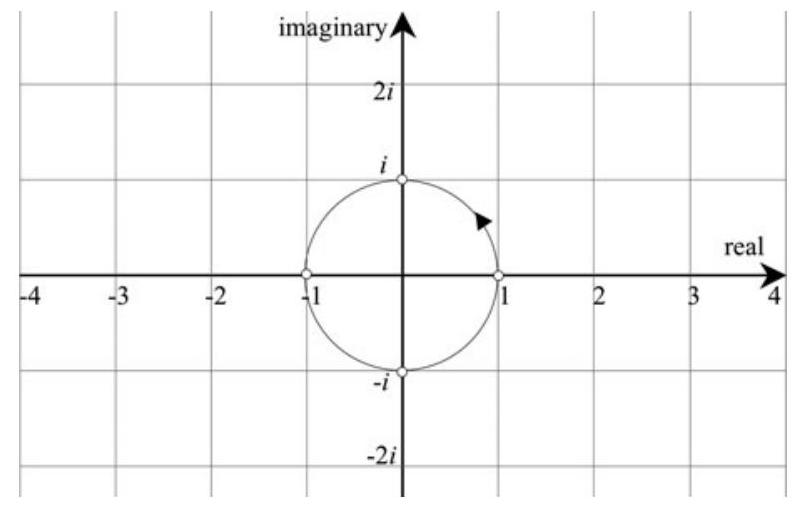
\includegraphics[max width=0.6\textwidth]{2023_01_16_a848224efad29cd66460g-050}
    \caption{带单位圆的复平面}
\end{figure}
它集成了5个重要常数:$0,1,e, \pi$和$i$,以及基本的算术运算:加法,乘法和求幂。

当$\theta=\pi / 2$时,这个公式会产生另一个结果:
$$
e^{i \pi / 2}=\cos \frac{\pi}{2}+i \sin \frac{\pi}{2}=i
$$
因此,\footnote{译者注,和网友讨论,并不止这一种结果,正确的结果应该如此:
\begin{align*}
    \begin{aligned}
        i &=  \cos (\frac{\pi}{2}+2k\pi)+i\sin(\frac{\pi}{2}+2k\pi)\\
        &=e^{i({\pi/2}+2k\pi)},\qquad k\in \mathbb{Z}\\
        i^i &= e^{-(\pi/2+2k\pi)},\qquad k\in \mathbb{Z}\\
    \end{aligned}
\end{align*}

是一个完全的实数的实数幂函数,对应多个值,感谢网友“天津-莲子粥(嵌入式)”。}

$$
\begin{aligned}
i^{i} & =\left(e^{i \pi / 2}\right)^{i} \\
& =e^{i^{2} \pi / 2} \\
& =e^{-\pi / 2} \\
& =0.207879576 \ldots
\end{aligned}
$$
这表明虚数单位自身的幂等于一个实数!\footnote{译者注,参考上一条脚注,应该是一系列实数。}

在第三章中,我们看到虚$i$的幂会产生两个序列$(1,i,-1,-i, 1, \ldots)$和$(1,-i,-1, i, 1, \ldots)$,它们与分别沿逆时针和顺时针方向绕笛卡尔轴旋转时产生的$(x, y,-x,-y, y, x, \ldots)$和$(x,-y,-x, y, x, \ldots)$的模式有着显著的相似之处。这种相似性并非巧合,因为复数属于一个叫做复平面的二维平面,我们现在将描述复平面。

复平面使我们能够可视化复数,横轴记录实数部分,纵轴记录虚数部分,如图4.1所示。该图还显示了一个以单位半径穿过点$1,i,-1,-i$的圆,这是与$i$的幂递增相关的序列。我们可以看到$i^{0}=1, i^{1}=i, i^{2}=-1, i^{3}=-i$和$i^{4}=1$的位置,这表明乘以$i$相当于旋转$90^{\circ}$。为了证明这种旋转效应,图4.2给出了包含四个复数的复平面:
$$
p=2+i, \quad q=-1+2 i, \quad r=-2-i, \quad s=1-2 i
$$
它们之间的距离是$90^{\circ}$。

\begin{figure}[h!]
    \centering
    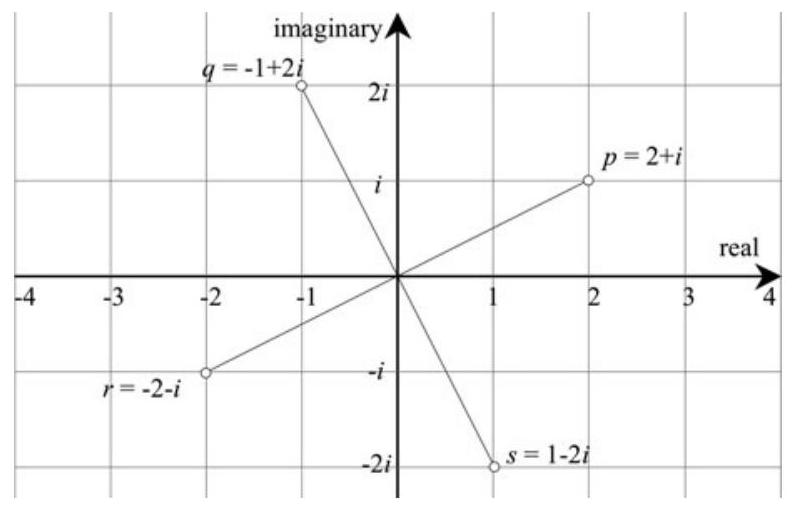
\includegraphics[max width=0.6\textwidth]{2023_01_16_a848224efad29cd66460g-051}
    \caption{标记4个复数的复平面}
\end{figure}

点$p$通过乘以$i$旋转$90^{\circ}$到$q$:
$$
\begin{aligned}
i(2+i) & =2 i+i^{2} \\
& =-1+2 i .
\end{aligned}
$$
点$q$通过乘以$i$旋转$90^{\circ}$到$r$:
$$
\begin{aligned}
i(-1+2 i) & =-i+2 i^{2} \\
& =-2-i .
\end{aligned}
$$
点$r$再乘以$i$旋转$90^{\circ}$到$s$:
$$
\begin{aligned}
i(-2-i) & =-2 i-i^{2} \\
& =1-2 i
\end{aligned}
$$
最后,点$s$乘以$i$被旋转$90^{\circ}$为$p$,:
$$
\begin{aligned}
i(1-2 i) & =i-2 i^{2} \\
& =2+i
\end{aligned}
$$

我们还在第三章中发现,与增加负幂相关的序列:$(1,-i,-1, i, \ldots)$是一个顺时针方向的旋转,这意味着将一个复数除以$i$将它顺时针旋转$90^{\circ}$。然而,我们证明了$i^{-1}=-i$,用$-i$乘以一个复数要比用$i$除以简单得多。所以让我们重复上面的练习来证明这一点。

点$p$乘以$-i$被旋转$-90^{\circ}$到$s$:
$$
\begin{aligned}
-i(2+i) & =-2 i-i^{2} \\
& =1-2 i .
\end{aligned}
$$
点$s$再乘以$-i$旋转$-90^{\circ}$到$r$:
$$
\begin{aligned}
-i(1-2 i) & =-i+2 i^{2} \\
& =-2-i .
\end{aligned}
$$
点$r$再乘以$-i$旋转$-90^{\circ}$到$q$,:
$$
\begin{aligned}
-i(-2-i) & =2 i+i^{2} \\
& =-1+2 i .
\end{aligned}
$$
最后,点$q$乘以$-i$被旋转$-90^{\circ}$为$p$:
$$
\begin{aligned}
-i(-1+2 i) & =i-2 i^{2} \\
& =2+i .
\end{aligned}
$$
因此,将一个复数旋转$\pm 90^{\circ}$,乘以$\pm i$。

在第3章中,我们看到$\sqrt{\pm i}$的根为
$$
\begin{aligned}
& \sqrt{+i}=\pm \frac{\sqrt{2}}{2}(1+i) \\
& \sqrt{-i}=\pm \frac{\sqrt{2}}{2}(1-i)
\end{aligned}
$$
请注意如图4.3所示,每个根之间的距离为$180^{\circ}$,这表明角度与它们的行为有关。例如,$\sqrt{+i}$的正根是$\sqrt{2}/ 2(1+i)$,离实轴为$45^{\circ}$。将这个根乘以它自己,将它$45^{\circ}$旋转到$i$轴。类似地,负根是$-\sqrt{2}/ 2(1+i)$,离实轴为$225^{\circ}$。这个根乘以它自己,将它$225^{\circ}$旋转到$i$轴。$\sqrt{-i}$的根也是如此。

\begin{figure}[h!]
    \centering
    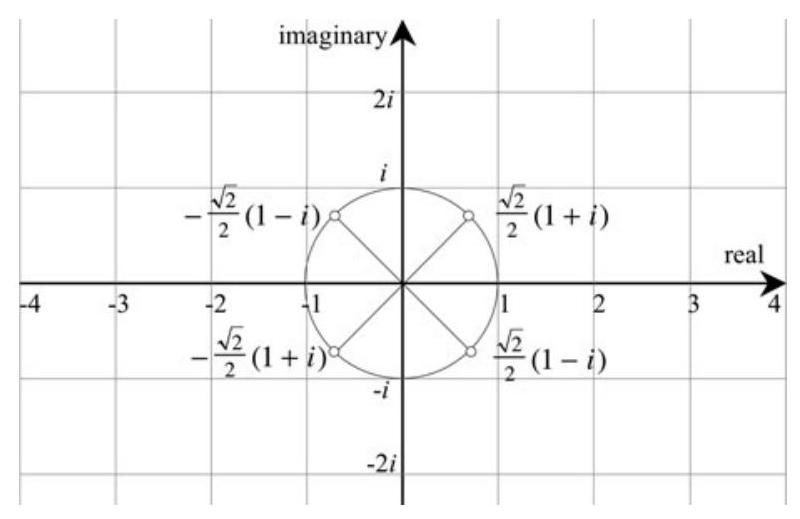
\includegraphics[max width=0.6\textwidth]{2023_01_16_a848224efad29cd66460g-052}
    \caption[short]{$\sqrt{\pm i}$的根}
\end{figure}

这些观察似乎表明,我们可以构造一个能够使另一个复数旋转任意角度的复数。这是真的,我们接下来会讲到。

\section{极坐标表示法}
在复平面上放置一个复数,我们得到极坐标表示,在极坐标表示中,我们从原点到复数形成一条直线,如图4.4所示。这条线的长度是$r$,等于$\sqrt{a^{2}+b^{2}}$,这就是为什么复数的范数是用毕达哥拉斯公式定义的:
\begin{figure}[h!]
    \centering
    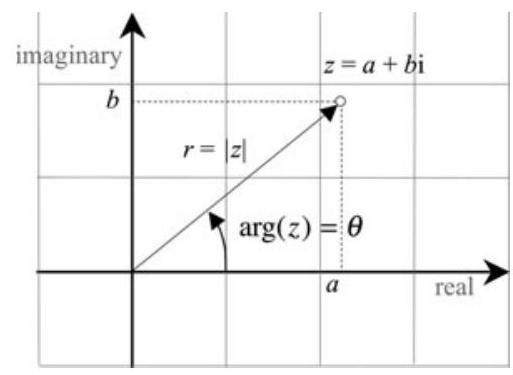
\includegraphics[max width=0.6\textwidth]{2023_01_16_a848224efad29cd66460g-053}
    \caption[short]{复数的极坐标表示
    }
\end{figure}

$$
r=|z|=\sqrt{a^{2}+b^{2}} .
$$
直线与实轴之间的角度$\theta$称为$z$的参数
$$
\arg (z)=\theta
$$
其中
$$
\tan \theta=\frac{b}{a} .
$$
我们计算$\arg (z)$使用
$$
\begin{array}{ll}
\text { 第一象限 } a>0, b>0 & \theta=\arctan (b / a) \\
\text { 第二和第三象限 } a<0 & \theta=\arctan (b / a)+\pi \\
\text { 第四象限 } a>0, b<0 & \theta=\arctan (b / a)+2 \pi .
\end{array}
$$
从图4.4中我们可以看到,z的水平分量是$r \cos \theta$,垂直分量是$r \sin \theta$,这使得我们可以写
$$
\begin{aligned}
z & =a+b i \\
& =r \cos \theta+r i \sin \theta \\
& =r(\cos \theta+i \sin \theta) .
\end{aligned}
$$
如上所述,欧拉的发现之一是关于$e^{\theta}, \sin \theta$和$ cos \theta$幂级数的恒等式:
$$
e^{i \theta}=\cos \theta+i \sin \theta
$$
这允许我们写作
$$
z=r e^{i \theta} .
$$
有了这个发现,我们现在可以用极坐标表示法来重新讨论两个复数的乘积和商。例如,给定下列复数
$$
\begin{aligned}
z & =r e^{i \theta} \\
w & =s e^{i \phi}
\end{aligned}
$$
他们的乘积
$$
\begin{aligned}
z w & =r s e^{i \theta} e^{i \phi} \\
& =r s e^{i(\theta+\phi)} \\
& =r s[\cos (\theta+\phi)+i \sin (\theta+\phi)]
\end{aligned}
$$
所以两个复数的乘积会产生第三个有范数的复数
$$
|z w|=r s
$$
且参数
$$
\arg (z w)=\theta+\phi
$$
这里两个角直接相加了。

接下来,除法:
$$
\begin{aligned}
\frac{z}{w} & =\frac{r e^{i \theta}}{s e^{i \phi}} \\
& =\frac{r}{s} e^{i(\theta-\phi)} \\
& =\frac{r}{s}[\cos (\theta-\phi)+i \sin (\theta-\phi)]
\end{aligned}
$$
其中,范数是
$$
\left|\frac{z}{w}\right|=\frac{r}{s}
$$
且参数为
$$
\arg (z / w)=\theta-\phi
$$
这里是两个角度相减了。

让我们用一个例子来应用这些公式。图$4.5$显示了两个复数
$$
\begin{gathered}
z=2+2 i \\
w=-1+i
\end{gathered}
$$
在极坐标形式里面是
$$
\begin{aligned}
z & =2 \sqrt{2}\left(\cos 45^{\circ}+i \sin 45^{\circ}\right)=2 \sqrt{2} e^{i \pi / 4} \\
w & =\sqrt{2}\left(\cos 135^{\circ}+i \sin 135^{\circ}\right)=\sqrt{2} e^{i 3 \pi / 4} .
\end{aligned}
$$
用普通的复代数,乘积$z w$是
$$
z w=(2+2 i)(-1+i)=-4
$$
\begin{figure}[h!]
    \centering
    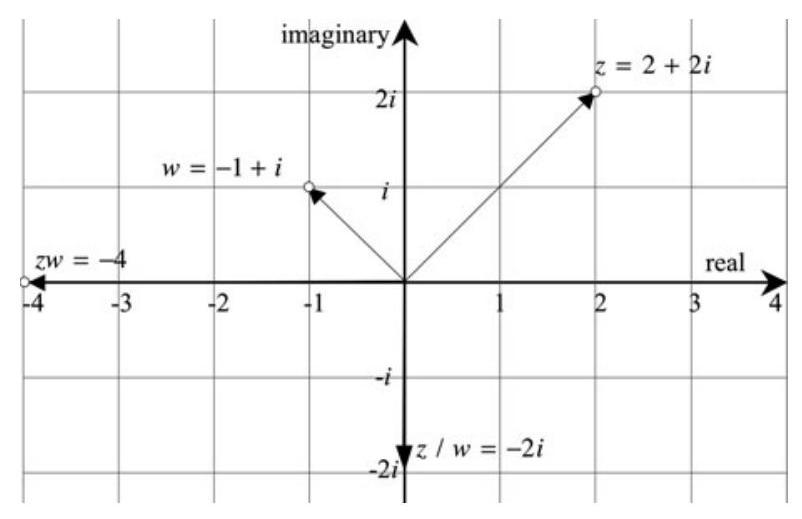
\includegraphics[max width=0.6\textwidth]{2023_01_16_a848224efad29cd66460g-055}
    \caption[short]{两个复数的乘积}
\end{figure}
用极坐标形式是:
$$
\begin{aligned}
|z w| & =2 \sqrt{2} \sqrt{2}=4 \\
\arg (z w) & =45^{\circ}+135^{\circ}=180^{\circ}
\end{aligned}
$$
这里编码为$-4$。

现在让我们用普通的复代数和极坐标形式来计算商$z / w$。
$$
\begin{aligned}
\frac{z}{w} & =\frac{(2+2 i)}{(-1+i)} \frac{(-1-i)}{(-1-i)} \\
& =\frac{-2-2 i-2 i-2 i^{2}}{1+1} \\
& =-2 i
\end{aligned}
$$
接下来,使用极坐标形式:
$$
\begin{aligned}
|z / w| & =\frac{2 \sqrt{2}}{\sqrt{2}}=2 \\
\arg (z / w) & =45^{\circ}-135^{\circ}=-90^{\circ}
\end{aligned}
$$
这编码复数$-2 i$。这些结果如图4.5所示。

我们还可以使用欧拉公式计算$\sqrt{i}$ ,如下所示
$$
e^{i \theta}=\cos \theta+i \sin \theta
$$
将$\theta=\pi / 2$代入
$$
e^{i \pi / 2}=\cos \frac{\pi}{2}+i \sin \frac{\pi}{2}=i
$$
两边同时开根号,得到
$$
\begin{aligned}
e^{i \pi / 4} & =\pm \sqrt{i} \\
\cos \frac{\pi}{4}+i \sin \frac{\pi}{4} & =\pm \sqrt{i} \\
\pm \frac{\sqrt{2}}{2}(1+i) & =\pm \sqrt{i}
\end{aligned}
$$
为了找到$\sqrt{-i}$,我们代入$\theta=-\pi / 2$:
$$
\begin{aligned}
e^{-i \pi / 2} & =\cos \left(-\frac{\pi}{2}\right)+i \sin \left(-\frac{\pi}{2}\right)=-i \\
& =\cos \left(\frac{\pi}{2}\right)-i \sin \left(\frac{\pi}{2}\right)=-i
\end{aligned}
$$
两边同时开根号,得到
$$
\begin{aligned}
e^{-i \pi / 4} & =\pm \sqrt{-i} \\
\cos \left(\frac{\pi}{4}\right)-i \sin \left(\frac{\pi}{4}\right) & =\pm \sqrt{-i} \\
\pm \frac{\sqrt{2}}{2}(1-i) & =\pm \sqrt{-i}
\end{aligned}
$$
用类似的方法可以找到更高次的根。

\section{转子}
极坐标形式说明了这样一个事实:范数为$r$的复数$z=r e^{i \theta}$与范数为$s$的复数$w=s e^{i \phi}$相乘,就得到了第三个范数为$r s$的复数。因此,为了避免缩放$z, w$必须有一个范数单位$1$。在这种情况下,$w$充当转子。例如,用$4+5 i$乘以$1+0 i$,它就没有缩放和旋转。然而,用$4+5 i$乘以$0+i$将它旋转$90^{\circ}$而不进行任何缩放。

因此,要将$2+2 i$旋转$45^{\circ}$,我们必须将它乘以$e^{i \pi / 4}$:
$$
\begin{aligned}
e^{i \pi / 4} & =\cos 45^{\circ}+i \sin 45^{\circ}=\frac{\sqrt{2}}{2}(1+i) \\
\frac{\sqrt{2}}{2}(1+i)(2+2 i) & =\frac{\sqrt{2}}{2} 4 i \\
& =2 \sqrt{2} i .
\end{aligned}
$$
因此$e^{i \theta}$将任何复数旋转一个角度$\theta$。

要使复数$x+y i$旋转一个角度$\theta$,我们可以将它乘以转子$\cos \theta+i \sin \theta$:
$$
\begin{aligned}
x^{\prime}+y^{\prime} i & =(\cos \theta+i \sin \theta)(x+y i) \\
& =x \cos \theta-y \sin \theta+i(x \sin \theta+y \cos \theta)
\end{aligned}
$$
矩阵形式是:
$$
\left[\begin{array}{cc}
x^{\prime} & -y^{\prime} \\
y^{\prime} & x^{\prime}
\end{array}\right]=\left[\begin{array}{cc}
\cos \theta & -\sin \theta \\
\sin \theta & \cos \theta
\end{array}\right]\left[\begin{array}{cc}
x & -y \\
y & x
\end{array}\right] .
$$
在继续之前,让我们考虑转子的复共轭对旋转方向的影响,我们可以通过将$x+y i$乘以转子$\cos \theta -i \sin \theta$来实现
$$
\begin{aligned}
x^{\prime}+y^{\prime} i & =(\cos \theta-i \sin \theta)(x+y i) \\
& =x \cos \theta+y \sin \theta-i(x \sin \theta+y \cos \theta)
\end{aligned}
$$
矩阵形式是
$$
\left[\begin{array}{cc}
x^{\prime} & -y^{\prime} \\
y^{\prime} & x^{\prime}
\end{array}\right]=\left[\begin{array}{cc}
\cos \theta & \sin \theta \\
-\sin \theta & \cos \theta
\end{array}\right]\left[\begin{array}{cc}
x & -y \\
y & x
\end{array}\right]
$$
也就是绕原点旋转$-\theta$。

因此,我们定义一个转子$\mathbf{R}_{\theta}$和它的共轭$\mathbf{R}_{\theta}^{\dagger}$为
$$
\begin{aligned}
& \mathbf{R}_{\theta}=\cos \theta+i \sin \theta \\
& \mathbf{R}_{\theta}^{\dagger}=\cos \theta-i \sin \theta
\end{aligned}
$$
其中$\mathbf {R} _{\theta}$旋转$+ \theta$,和$\mathbf{R}_{\theta}^{\dagger}$旋转$- \theta$。注意,使用了匕首$\dagger$符号。

\section{总结}
在本章中,我们发现了用复平面来表示复数的图形化解释。欧拉公式$e^{i \theta}=\cos \theta+i \sin \theta$允许我们将复数表示为$e$的虚数次幂,从而使我们可以轻松地计算乘积和商。总的来说,这些想法把我们引向了转子的想法,它将使用四元数来开发。

\subsection{运算符总结}
\subsubsection*{复数}
$$
\begin{aligned}
z & =a+b i \\
|z| & =\sqrt{a^{2}+b^{2}}
\end{aligned}
$$

\subsubsection*{极坐标表示}

$$
\begin{aligned}
z & =r e^{i \theta} \\
z & =r(\cos \theta+i \sin \theta) \\
r & =|z| \\
\tan \theta & =b / a \\
\theta & =\arg (z)
\end{aligned}
$$

\begin{align*}
    \begin{aligned}
        &\text{第一象限  } a>0, b>0 && \theta=\arctan (b / a)\\
        &\text{第二和第三象限  } a<0 && \theta=\arctan (b / a)+\pi\\
        &\text{第四象限  } a>0, b<0 && \theta=\arctan (b / a)+2 \pi.
    \end{aligned}
\end{align*}


\subsubsection*{乘积}
$$
\begin{aligned}
z & =r e^{i \theta} \\
w & =s e^{i \phi} \\
z w & =r s e^{i(\theta+\phi)} \\
& =r s[\cos (\theta+\phi)+i \sin (\theta+\phi)]
\end{aligned}
$$

\subsubsection*{商}
$$
\begin{aligned}
\frac{z}{w} & =\frac{r}{s} e^{i(\theta-\phi)} \\
& =\frac{r}{s}[\cos (\theta-\phi)+i \sin (\theta-\phi)]
\end{aligned}
$$

\subsubsection*{转子}
$$
\begin{aligned}
& \mathbf{R}_{\theta}=\cos \theta+i \sin \theta \\
& \mathbf{R}_{\theta}^{\dagger}=\cos \theta-i \sin \theta
\end{aligned}
$$

\section{样例}
下面是一些进一步使用上述思想的示例。在某些情况下,包括测试来确认结果。
\begin{example}
    
    从$1+2 i$开始,将得到的复数乘以$i$四次,并将结果绘制在复平面上。
    
    点$p$通过乘以$i$旋转$90^{\circ}$到$q$:
    $$
    \begin{aligned}
    i(1+2 i) & =i+2 i^{2} \\
    & =-2+i .
    \end{aligned}
    $$
    
    点$q$通过乘以$i$旋转$90^{\circ}$到$r$:
    $$
    \begin{aligned}
    i(-2+i) & =-2 i+i^{2} \\
    & =-1-2 i
    \end{aligned}
    $$
    
    点$r$再乘以$i$旋转$90^{\circ}$到$s$:
    $$
    \begin{aligned}
    i(-1-2 i) & =-i-2 i^{2} \\
    & =2-i .
    \end{aligned}
    $$
    
    最后,点$s$乘以$i$被旋转$90^{\circ}$为$p$:
    $$
    \begin{aligned}
    i(2-i) & =2 i-i^{2} \\
    & =2+i .
    \end{aligned}
    $$
    
    图$4.6$显示了四个被$90^{\circ}$隔开的复数。
    \begin{figure}[h!]
        \centering
        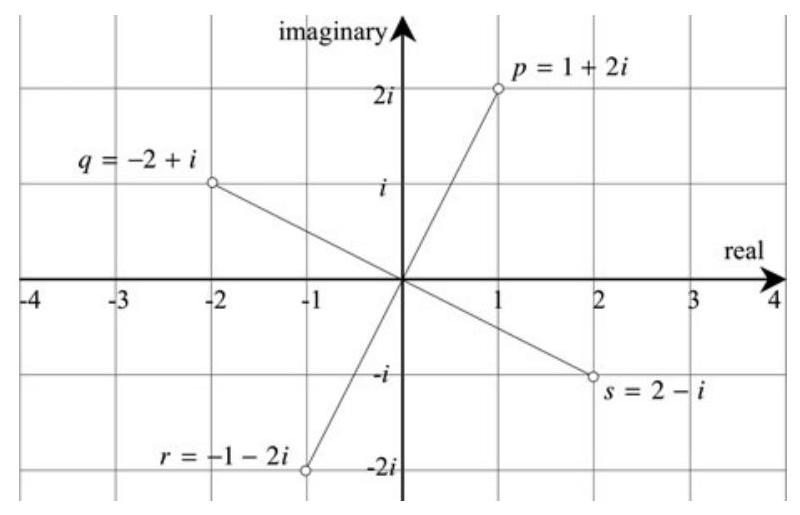
\includegraphics[max width=0.6\textwidth]{2023_01_16_a848224efad29cd66460g-059}
        \caption{有四个复数的复平面}
    \end{figure}
\end{example}

\begin{example}
    用极坐标形式计算乘积$ zw $和商$z / w$。
    $$
    \begin{gathered}
    z=3+3 i \\
    w=-1-i
    \end{gathered}
    $$
    
    乘积:
    $$
    \begin{aligned}
    z & =3 \sqrt{2}\left(\cos 45^{\circ}+i \sin 45^{\circ}\right)=3 \sqrt{2} e^{i \pi / 4} \\
    w & =\sqrt{2}\left(\cos 225^{\circ}+i \sin 225^{\circ}\right)=\sqrt{2} e^{i 5 \pi / 4} \\
    |z w| & =3 \sqrt{2} \sqrt{2}=6 \\
    \arg (z w) & =45^{\circ}+225^{\circ}=270^{\circ}
    \end{aligned}
    $$
    这编码复数$-6 i$。
    
    测试:使用普通的复代数,乘积$ zw $为
    $$
    z w=(3+3 i)(-1-i)=-6 i .
    $$
    
    商:
    $$
    \begin{aligned}
    |z| & =3 \sqrt{2} \\
    |w| & =\sqrt{2} \\
    |z / w| & =3 \sqrt{2} / \sqrt{2}=3 \\
    \arg (z / w) & =45^{\circ}-225^{\circ}=180^{\circ}
    \end{aligned}
    $$
    这编码复数$-3$.
    
    测试:使用普通的复代数,乘积$ z/w $为
    $$
    \begin{aligned}
    \frac{z}{w} & =\frac{(3+3 i)}{(-1-i)} \frac{(-1+i)}{(-1+i)} \\
    & =\frac{-6}{2} \\
    & =-3
    \end{aligned}
    $$
    
    并且符合极坐标形式。
\end{example}

\begin{example}
    设计一个转子,将一个复数旋转$30^{\circ}$而不缩放。
    
    这样开始
    $$
    e^{i \theta}=\cos \theta+i \sin \theta
    $$
    
    令 $\theta=30^{\circ}=\pi / 6$
    $$
    \begin{aligned}
    e^{i \pi / 6} & =\cos 30^{\circ}+i \sin 30^{\circ} \\
    & =\frac{\sqrt{3}}{2}+i \frac{1}{2} \\
    & =\frac{1}{2}(\sqrt{3}+i) .
    \end{aligned}
    $$
    
    测试:让我们用这个转子将$1+0 i$旋转三次到$i$。
    $$
    \begin{aligned}
    \frac{1}{2}(\sqrt{3}+i) \frac{1}{2}(\sqrt{3}+i) \frac{1}{2}(\sqrt{3}+i) 1 & =\frac{1}{8}(\sqrt{3}+i)(\sqrt{3}+i)(\sqrt{3}+i) \\
    & =\frac{1}{8}(2+2 \sqrt{3} i)(\sqrt{3}+i) \\
    & =\frac{1}{8}(2 \sqrt{3}-2 \sqrt{3}+2 i+6 i) \\
    & =i
    \end{aligned}
    $$
\end{example}

\begin{example}
    设计一个转子,将一个复数旋转$-60^{\circ}$而不缩放。
    
    这样开始
    $$
    e^{i \theta}=\cos \theta+i \sin \theta
    $$
    
    令 $\theta=-60^{\circ}=-\pi / 3$
    
    $$
    \begin{aligned}
    e^{-i \pi / 3} & =\cos \left(-60^{\circ}\right)+i \sin \left(-60^{\circ}\right) \\
    & =\frac{1}{2}-\frac{\sqrt{3}}{2} i \\
    & =\frac{1}{2}(1-\sqrt{3} i)
    \end{aligned}
    $$
\end{example}


\chap{四元数代数}
\section{介绍}
当一群杰出的数学家对同一学科感兴趣时,发现其中两个人同时提出同样的发明是很常见的。即使两个这样的人有不同的数学特长,他们也应该有机会获得相同的数学知识积累,并意识到已经解决的问题和正在等待解决的问题。

在第四章中,我们看到Wessel和Argand都发明了复平面,并用它来表示复数。不幸的是,他们都无法接触到当今无处不在的出版网络和全球网络。然而,优先权过去是——现在仍然是——由谁先出版决定的。但正如我们在Wessel身上看到的,即使是第一次出版也不能保证成名。

四元数的发明也有类似的故事。William Rowan Hamilton爵士被公认为四元数代数的发明者,这是第一个被发现的非交换代数。人们可以想象,当他找到了一个他思考了十年的问题的解决方案时,他有多高兴!

这项发明为操纵矢量提供了第一个数学框架,尽管这是由美国理论物理学家、化学家和数学家乔西亚·威拉德·吉布斯(Josiah Willard Gibbs, 1839-1903)改进的。虽然汉密尔顿是通过代数途径得到他的发明的,但对他来说,四元数显然具有重要的几何潜力,他立即开始探索它们的矢量和旋转性质。

Hamilton和当时几乎所有人都不知道,法国社会改革家、杰出的业余数学家本杰明·奥林德·罗德里格斯(Benjamin Olinde Rodrigues, 1795-1851)已经在1840年发表了一篇论文,描述了如何用围绕第三个轴[9]的一次旋转来表示围绕不同轴的两次连续旋转。更重要的是,Rodrigues使用标量和3D轴来表达他的解决方案,这比Hamilton自己使用标量和向量的方法早了三年!西蒙·奥特曼(Simon Altmann)可能比其他任何人都更努力地澄清这一事实,并广泛发表了他的观点[1,3 -5]。然而,现在,让我们继续Hamilton的代数,并在第六章和Rodrigues博士一起回到它的旋转性质。

复数的存在给18和19世纪的数学家们带来了一个诱人的问题。能否有一个三维等价物?这个问题的答案并不明显,许多有天赋的数学家,包括Gauss, Möbius, Grassmann, 和 Hamilton都在寻找答案。

Hamilton的研究有据可查,涵盖了从19世纪30年代初到1843年的一段时间,当时他发明了四元数。在接下来的22年里,直到他1865年去世,他一直专注于这个课题。到1833年,他已经证明复数形成了一个对偶的代数,即有序的对[14]。

由于二维复数由$a+b i$表示,Hamilton猜想三维复数可以由$a+b i+c j$的三联体表示,其中$i$和$j$是虚量,且平方为$-1$。然而,两个这样的三联体的乘积引起了它们的代数扩展问题。
$$
\begin{aligned}
z_{1}= & a_{1}+b_{1} i+c_{1} j \\
z_{2}= & a_{2}+b_{2} i+c_{2} j \\
z_{1} z_{2}= & \left(a_{1}+b_{1} i+c_{1} j\right)\left(a_{2}+b_{2} i+c_{2} j\right) \\
= & a_{1} a_{2}+a_{1} b_{2} i+a_{1} c_{2} j \\
& +b_{1} a_{2} i+b_{1} b_{2} i^{2}+b_{1} c_{2} i j+c_{1} a_{2} j+c_{1} b_{2} j i+c_{1} c_{2} j^{2} \\
= & \left(a_{1} a_{2}-b_{1} b_{2}-c_{1} c_{2}\right)+\left(a_{1} b_{2}+b_{1} a_{2}\right) i+\left(a_{1} c_{2}+c_{1} a_{2}\right) j \\
& +b_{1} c_{2} i j+c_{1} b_{2} j i
\end{aligned}
$$

除了涉及$i j$和$j i$的项外,这个操作几乎是封闭的。即使我们假设$j i=-i j$,我们仍然剩下
$$
\left(b_{1} c_{2}-c_{1} b_{2}\right) i j .
$$

这给Hamilton带来了一个真正的问题,他花了十多年的时间试图解决这个问题。然后,在1843年10月16日,当他和妻子Hamilton夫人沿着爱尔兰皇家运河散步,主持爱尔兰皇家学院的一次会议时,他灵光一闪,想到了解决方案:四重组合,而不是三重组合。而不是使用两个虚构的项,三个项提供了必要的额外排列来解析像$i j$这样的乘积。

这方案是$z=a+ bi +c j+d k$,其中$i, j, k$的平方都为$-1$。因为这四项, Hamilton 把四元数命名为四元数。Hamilton抓住这个机会把比赛记录在石头上,他把计算法则刻在了布鲁姆(Broome)桥的墙上,当时他正在路过这座桥。尽管他最初的铭文没有经受住爱尔兰多年的风雨,但现在有一块更永久的铭牌取代了它。

当Hamilton 发明四元数时,他还创造了各种各样的名称,如张量、维数和向量来描述它们的属性。作为发明者, Hamilton 有权选择任何他想要的名字,在当时,这样的名字与那个时期的符号有关。例如,他称四元数的实部为标量,虚部为向量。然而今天,向量没有任何想象的关联,这使得四元数的解释有点混乱。

Simon Altmann 非常清楚这些问题,并通过对四元数代数进行仔细审查来帮助澄清这种困惑,这是迄今为止所缺乏的。这种代数的严密性采用了有序对的思想,这很容易理解,并揭示了四元数和复数之间的密切关系。

让我们研究一下四元数的代数,它构成了集合$\mathbb{H}$,以表彰 Hamilton 的成就。

\section{一点历史}
Hamilton定义了四元数$q$,其相关规则为
$$
q=s+i a+j b+k c \quad s, a, b, c \in \mathbb{R}
$$

且
$$
\begin{gathered}
i^{2}=j^{2}=k^{2}=i j k=-1 \\
i j=k, \quad j k=i, \quad k i=j \\
j i=-k, \quad k j=-i, \quad i k=-j
\end{gathered}
$$

[16-18],但我们倾向于写作四元数
$$
q=s+a i+b j+c k .
$$

从Hamilton的规则中观察$i j$是如何被$k$取代的。额外的虚数$k$项是循环模式$i j=k, j k=i$和$k i=j$的关键,它们非常类似于两个单位笛卡尔向量的外积:
$$
\mathbf{i} \times \mathbf{j}=\mathbf{k}, \quad \mathbf{j} \times \mathbf{k}=\mathbf{i}, \quad \mathbf{k} \times \mathbf{i}=\mathbf{j} .
$$

事实上,这种相似性并非巧合,因为 Hamilton 还发明了标量积和向量积。然而,尽管四元数提供了一个描述向量的代数框架,人们必须承认,在 Hamilton 之前,矢量已经被研究了很多年。

Hamilton 还看到$i, j, k$项可以表示三个笛卡尔单位向量$\mathbf{i}, \mathbf{j}$和$\mathbf{k}$,它们必须具有虚数性质。例如,$\mathbf{i}^{2}=-1$等,一些数学家和科学家并不认同,他们怀疑需要涉及这么多虚数项。

Hamilton 寻找复数的三维等效的动机部分是代数的,部分是几何的。因为,如果一个复数是由一对数表示的,并且能够将平面上的点旋转$90^{\circ}$,那么也许一个三重数可以将空间中的点旋转$90^{\circ}$。最后,三位数必须被四位数-四元数所取代。

\begin{figure}[h!]
    \centering
    \subfigure[]{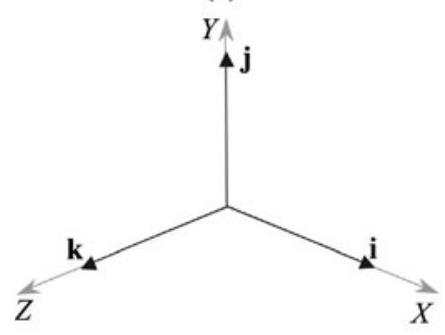
\includegraphics[max width=0.3\textwidth]{2023_01_16_a848224efad29cd66460g-065}}
    \subfigure[]{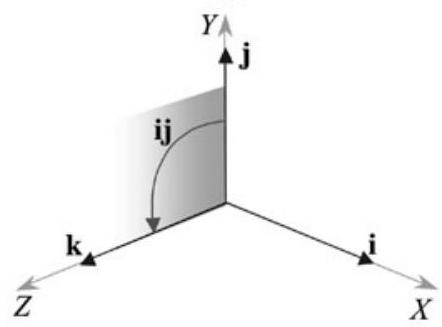
\includegraphics[max width=0.3\textwidth]{2023_01_16_a848224efad29cd66460g-065(2)}}\\
    \subfigure[]{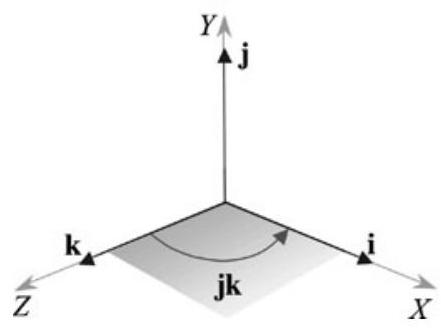
\includegraphics[max width=0.3\textwidth]{2023_01_16_a848224efad29cd66460g-065(1)}}
    \subfigure[]{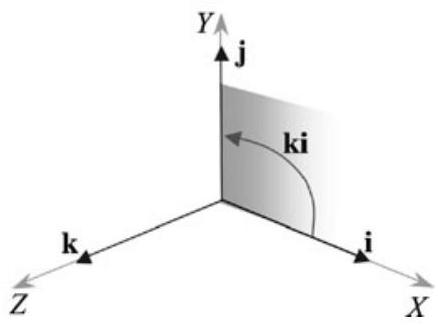
\includegraphics[max width=0.3\textwidth]{2023_01_16_a848224efad29cd66460g-065(3)}}
    \caption[short]{解释乘积$\mathbf{i j}, \mathbf{j} \mathbf{k}, \mathbf{k i}$}
\end{figure}

人们可以从两个角度来看待 Hamilton 的规则。第一,它们是结合三个虚数项的代数结果。第二,它们反映了空间的潜在几何结构。后一种解释被 P.G.Tait 采用,并在他的书《四元数概论》[21]中概述。 Tait 的方法假设三个单位向量$\mathbf{i}, \mathbf{j}, \mathbf{k}$分别与$x-, y$-, $z$-轴对齐:

\begin{CJK}{UTF8}{gkai}
    “将$\mathbf{i}$乘以$\mathbf{j}$或$\mathbf{i} \mathbf{j}$的结果被定义为$\mathbf{j}$在垂直于$\mathbf{i}$的平面上沿正方向旋转一个直角,换句话说,$\mathbf{i}$对$\mathbf{j}$的操作将其旋转,使其与$\mathbf{k}$重合;因此简单地$\mathbf{i j}=\mathbf{k}$。

    为了保持一致,必须承认,如果$\mathbf{i}$操作的不是$\mathbf{j}$,而是在平面$ yz $中操作与$\mathbf{i}$垂直的任何其他单位向量,它将使其沿同一方向旋转一个直角,因此$\mathbf{i k}$只能是$-\mathbf{j}$。

    将我们通过引用$\mathbf{i}$所说明的定义扩展到其他单位向量,很明显,$\mathbf{j}$作用于$\mathbf{k}$一定会得到$\mathbf{i}$,或$\mathbf{j} \mathbf{k}=\mathbf{i}$。”
\end{CJK}

Tait的解释见图$5.1$ (a)-(d)。图$5.1$ (a)显示了$\mathbf{i}, \mathbf{j}, \mathbf{k}$的原始对齐方式。图$5.1$ (b)显示了将$\mathbf{j}$转换为$\mathbf{k}$的效果。图$5.1$ (c)显示$\mathbf{k}$变为$\mathbf{i}$,图$5.1$ (d)显示$\mathbf{i}$变为$\mathbf{j}$。

到目前为止,我们还没有提到虚量——我们只有:
$$
\begin{array}{ll}
\mathbf{i j}=\mathbf{k}, & \mathbf{j} \mathbf{k}=\mathbf{i}, \quad \mathbf{k i}=\mathbf{j} \\
\mathbf{j} \mathbf{i}=-\mathbf{k}, & \mathbf{k j}=-\mathbf{i}, \quad \mathbf{i k}=-\mathbf{j}
\end{array}
$$

如果我们假设这些向量服从代数的分配律和结合律,它们的虚数性质就暴露出来了。例如:
$$
\mathbf{i j}=\mathbf{k}
$$

和都乘以$\mathbf{i}$:
$$
\mathbf{i}\mathbf{i} \mathbf{j}=\mathbf{i k}=-\mathbf{j}
$$

因此,
$$
\mathbf{i i}=\mathbf{i}^{2}=-1 .
$$

同样,我们可以展示$\mathbf{j}^{2}=\mathbf{k}^{2}=-1$。

接下来:
$$
\mathbf{i j k}=\mathbf{i}(\mathbf{j k})=\mathbf{i} \mathbf{i}=\mathbf{i}^{2}=-1 .
$$

因此,仅仅通过声明叉乘的作用, Hamilton 的规则就出现了,以及它们所有的虚数特征。 Tait 还提出以下看法:

\begin{CJK}{UTF8}{gkai}
    “由Servois于1813年发表在 Gergonne 的年鉴上的一篇非常奇怪的推测是迄今为止发现的唯一一篇,其中包含了四元数预测的最轻微痕迹。他力图将平面的形式$a+b \sqrt{-1}$扩展到空间中,通过类推的方法在空间中写出有向的单位线
$$
p \cos \alpha+q \cos \beta+r \cos \gamma,
$$

其中$\alpha, \beta, \gamma$是它对三个轴的倾斜度。他很容易看出$p, q, r$一定是非实数:但是,他问道:“它们是虚的可约化为一般形式$A+B \sqrt{-1}$吗?”\footnote{"seraient-elles imaginaires réductibles à la forme générale $A+B \sqrt{-1}$ ?"} 这可能不是答案。事实上,它们是四元数演算的$\mathbf{i}, \mathbf{j}, \mathbf{k}$。”
\end{CJK}

因此,法国数学家 François-Joseph Servois(1768-1847)是另一个非常接近发现四元数的人。此外,泰特和汉密尔顿显然都不知道罗德里格斯发表的论文。

而且还不止于此。杰出的德国数学家卡尔·弗里德里希·高斯(karl Friedrich Gauss, 1777-1855)非常谨慎,害怕发表任何过于革命性的东西,以防他被同行的数学家嘲笑。他的日记显示,他在尼古拉·伊万诺维奇·洛巴切夫斯基(Nikolai Ivanovich Lobachevsky)之前就预见到了非欧几里得几何。他在1819年的日记中写道,他发现了一种方法,可以求出两个四重数$(a, b, c, d)$和$(\alpha, \beta, \gamma, \delta)$的乘积:
$$
\begin{aligned}
(A, B, C, D)= & (a, b, c, d)(\alpha, \beta, \gamma, \delta) \\
= & (a \alpha-b \beta-c \gamma-d \delta, a \beta+b \alpha-c \delta+d \gamma, \\
& a \gamma+b \delta+c \alpha-d \beta, a \delta-b \gamma+c \beta+d \alpha) .
\end{aligned}
$$

乍一看,这个结果看起来不像四元数乘积,但如果我们转置四元组的第二个和第三个坐标,并将它们视为四元数,我们就有
$$
\begin{aligned}
(A, B, C, D) & =(a+c i+b j+d k)(\alpha+\gamma i+\beta j+\delta k) \\
& =a \alpha-c \gamma-b \beta-d \delta+a(\gamma i+\beta j+\delta k) \\
& =+\alpha(c i+b j+d k),(b \delta-d \beta) i+(d \gamma-c \delta) j+(c \beta-b \gamma) k
\end{aligned}
$$

这和 Hamilton 的四元数积是一样的!此外,高斯还认识到这个乘积是非交换的。然而,他并没有发表他的发现,而是让汉密尔顿为自己发明了四元数,发表了他的结果,并获得了荣誉。

1881年和1884年,耶鲁大学的乔赛亚·威拉德·吉布斯(Josiah Willard Gibbs)为他的学生打印了关于矢量分析的课堂笔记。吉布斯割断了四元数的实数部分和向量部分之间的“脐带”,并提出了三维向量作为一个独立的对象,没有任何虚数的内涵。吉布斯还采纳了德国数学家赫尔曼Günter格拉斯曼(Hermann Günter Grassmann, 1809-1877)的思想,格拉斯曼自1832年以来一直在发展他自己的向量系统思想。Gibbs还使用四元数积的相关部分定义了标量积和向量积。最后,在1901年,吉布斯的学生埃德温·比德韦尔·威尔逊(Edwin Bidwell Wilson)以书的形式出版了吉布斯的笔记:向量分析[23],其中包含了今天使用的符号。

四元数代数绝对是虚的,但仅仅通过分离向量部分并忽略虚数规则, Gibbs 就能够揭示一个新的数学分支,它爆发为向量分析。

Hamilton 和他的支持者无法说服他们的同行,四元数可以表示矢量,最终,吉布斯的符号赢得了胜利,四元数淡出了舞台。

近年来,四元数被飞行模拟行业重新发现,最近又被计算机图形社区发现,它们被用于围绕任意轴旋转向量。在这期间,许多人都有机会研究代数,并提出利用代数特性的新方法。

让我们看看四元数$q$的三种写法:
\begin{align}
q= & s+x i+y j+z k \\
q= & s+\mathbf{v} \\
q= & {[s, \mathbf{v}] } \\
& \text { where } s, x, y, z \in \mathbb{R}, \quad \mathbf{v} \in \mathbb{R}^{3} \notag\\
& \text { and } i^{2}=j^{2}=k^{2}=-1 .\notag
\end{align}

区别是相当微妙的。在(5.1)中,我们有 Hamilton 的原始定义及其虚数术语和相关规则。在(5.2)中,' $+$ '符号用于向向量添加标量,这看起来很奇怪,但却有效。在(5.3)中,我们有一个由标量和向量组成的有序对。

现在你可能会想:同一个物体怎么可能有三种不同的定义?我认为你可以随便叫一个对象,只要它们在代数上是相同的。例如,用矩阵表示法表示一组线性方程,得到的结果与日常方程相同。因此,两种表示法是同样有效的。

虽然我在其他出版物中使用了(5.1)和(5.2)中的符号,但在本书中我使用的是有序对。因此,我们需要证明的是, Hamilton 对四元数的原始定义(5.1),包括它的标量和三个虚数项,可以被一个由标量和一个“现代”向量组成的有序对(5.3)所取代。

\section{定义四元数}
让我们从两个四元数$q_{a}$和$q_{b}$ à la Hamilton开始:\footnote{译注,原句是:Let's start with two quaternions $q_{a}$ and $q_{b}$ à la Hamilton:,感觉原句有错误排过来的字符。 }


$$
\begin{aligned}
& q_{a}=s_{a}+x_{a} i+y_{a} j+z_{a} k \\
& q_{b}=s_{b}+x_{b} i+y_{b} j+z_{b} k
\end{aligned}
$$

强制性的规则是:
% and the obligatory rules:
$$
\begin{gathered}
i^{2}=j^{2}=k^{2}=i j k=-1 \\
i j=k, \quad j k=i, \quad k i=j \\
j i=-k, \quad k j=-i, \quad i k=-j .
\end{gathered}
$$

我们的目标是证明$q_{a}$和$q_{b}$也可以用有序对表示
$$
\begin{aligned}
q_{a} & =\left[s_{a}, \mathbf{a}\right] \\
q_{b} & =\left[s_{b}, \mathbf{b}\right] \quad s_{a}, s_{b} \in \mathbb{R}, \quad \mathbf{a}, \mathbf{b} \in \mathbb{R}^{3} .
\end{aligned}
$$

我使用方括号作为定义的一部分,因为括号经常用于在四元数中分隔表达式。
% I have employed square brackets as part of the definition as parentheses are often used to delimit expressions within a quaternion.

四元数乘积$q_{a} q_{b}$展开为
\begin{align}
    \begin{aligned}
        q_{a} q_{b}=\left[s_{a}, \mathbf{a}\right]\left[s_{b}, \mathbf{b}\right]= & \left(s_{a}+x_{a} i+y_{a} j+z_{a} k\right)\left(s_{b}+x_{b} i+y_{b} j+z_{b} k\right) \\
        = & \left(s_{a} s_{b}-x_{a} x_{b}-y_{a} y_{b}-z_{a} z_{b}\right) \\
        & +\left(s_{a} x_{b}+s_{b} x_{a}+y_{a} z_{b}-y_{b} z_{a}\right) i \\
        & +\left(s_{a} y_{b}+s_{b} y_{a}+z_{a} x_{b}-z_{b} x_{a}\right) j \\
        & +\left(s_{a} z_{b}+s_{b} z_{a}+x_{a} y_{b}-x_{b} y_{a}\right) k
        \end{aligned}
\end{align}

式(5.4)采用另一个四元数的形式,证实四元数乘积是封闭的。

在此阶段,Hamilton将虚数$i, j, k$转换为单位笛卡尔向量$\mathbf{i}, \mathbf{j}, \mathbf{k}$,并将(5.4)转换为向量形式。这种方法的问题是向量保留了它们的虚根。Simon Altmann的建议是将虚数替换为有序对:
$$
i=[0, \mathbf{i}] \quad j=[0, \mathbf{j}] \quad k=[0, \mathbf{k}]
$$

它们本身就是四元数,叫做四元数单位。用四元数单位定义四元数的思想与用单位笛卡尔向量定义向量的思想完全相同。此外,它允许向量在没有任何虚数关联的情况下存在。

让我们用(5.4)中的这些四元数单位和$[1,\mathbf{0}]=1$替换:
\begin{align}
    \begin{aligned}
        {\left[s_{a}, \mathbf{a}\right]\left[s_{b}, \mathbf{b}\right]=} & \left(s_{a} s_{b}-x_{a} x_{b}-y_{a} y_{b}-z_{a} z_{b}\right)[1, \mathbf{0}] \\
        & +\left(s_{a} x_{b}+s_{b} x_{a}+y_{a} z_{b}-y_{b} z_{a}\right)[0, \mathbf{i}] \\
        & +\left(s_{a} y_{b}+s_{b} y_{a}+z_{a} x_{b}-z_{b} x_{a}\right)[0, \mathbf{j}] \\
        & +\left(s_{a} z_{b}+s_{b} z_{a}+x_{a} y_{b}-x_{b} y_{a}\right)[0, \mathbf{k}] .
    \end{aligned}
\end{align}



接下来,我们使用之前定义的规则展开(5.5):
\begin{align}
    \begin{aligned}
        {\left[s_{a}, \mathbf{a}\right]\left[s_{b}, \mathbf{b}\right]=} & {\left[s_{a} s_{b}-x_{a} x_{b}-y_{a} y_{b}-z_{a} z_{b}, \mathbf{0}\right] } \\
        & +\left[0,\left(s_{a} x_{b}+s_{b} x_{a}+y_{a} z_{b}-y_{b} z_{a}\right) \mathbf{i}\right] \\
        & +\left[0,\left(s_{a} y_{b}+s_{b} y_{a}+z_{a} x_{b}-z_{b} x_{a}\right) \mathbf{j}\right] \\
        & +\left[0,\left(s_{a} z_{b}+s_{b} z_{a}+x_{a} y_{b}-x_{b} y_{a}\right) \mathbf{k}\right] .
    \end{aligned} 
\end{align}

(5.6)的垂直扫描显示了一些隐藏的向量:
\begin{align}
    \begin{aligned}
        {\left[s_{a}, \mathbf{a}\right]\left[s_{b}, \mathbf{b}\right]=} & {\left[s_{a} s_{b}-x_{a} x_{b}-y_{a} y_{b}-z_{a} z_{b}, \mathbf{0}\right] } \\
        & +\left[0, s_{a}\left(x_{b} \mathbf{i}+y_{b} \mathbf{j}+z_{b} \mathbf{k}\right)+s_{b}\left(x_{a} \mathbf{i}+y_{a} \mathbf{j}+z_{a} \mathbf{k}\right)\right. \\
        & \left.+\left(y_{a} z_{b}-y_{b} z_{a}\right) \mathbf{i}+\left(z_{a} x_{b}-z_{b} x_{a}\right) \mathbf{j}+\left(x_{a} y_{b}-x_{b} y_{a}\right) \mathbf{k}\right] .
    \end{aligned}
\end{align}

式(5.7)包含两个有序对,现在可以组合:
\begin{align}
    \begin{aligned}
        {\left[s_{a}, \mathbf{a}\right]\left[s_{b}, \mathbf{b}\right]=} & {\left[s_{a} s_{b}-x_{a} x_{b}-y_{a} y_{b}-z_{a} z_{b},\right.} \\
        & s_{a}\left(x_{b} \mathbf{i}+y_{b} \mathbf{j}+z_{b} \mathbf{k}\right)+s_{b}\left(x_{a} \mathbf{i}+y_{a} \mathbf{j}+z_{a} \mathbf{k}\right) \\
        & \left.+\left(y_{a} z_{b}-y_{b} z_{a}\right) \mathbf{i}+\left(z_{a} x_{b}-z_{b} x_{a}\right) \mathbf{j}+\left(x_{a} y_{b}-x_{b} y_{a}\right) \mathbf{k}\right] .
    \end{aligned}
\end{align}

如果我们令
$$
\begin{aligned}
& \mathbf{a}=x_{a} \mathbf{i}+y_{a} \mathbf{j}+z_{a} \mathbf{k} \\
& \mathbf{b}=x_{b} \mathbf{i}+y_{b} \mathbf{j}+z_{b} \mathbf{k}
\end{aligned}
$$

代入(5.8)得到:
\begin{align}
    \left[s_{a}, \mathbf{a}\right]\left[s_{b}, \mathbf{b}\right]=\left[s_{a} s_{b}-\mathbf{a} \cdot \mathbf{b}, s_{a} \mathbf{b}+s_{b} \mathbf{a}+\mathbf{a} \times \mathbf{b}\right]
\end{align}

它定义了四元数乘积。

从现在开始,我们不必担心 Hamilton 的规则,因为它们嵌入在(5.9)中。此外,我们的向量没有虚数的关联。

虽然Rodrigues没有使用(5.9)中使用的Gibbs向量符号,但他设法计算出等效的代数表达式,这是一项成就。

\subsection{四元数单位}
使用(5.9),我们可以通过对四元数单位进行平方来检查四元数单位是否为虚数:
$$
\begin{aligned}
i & =[0, \mathbf{i}] \\
i^{2} & =[0, \mathbf{i}][0, \mathbf{i}] \\
& =[\mathbf{i} \cdot \mathbf{i}, \mathbf{i} \times \mathbf{i}] \\
& =[-1, \mathbf{0}]
\end{aligned}
$$

这是一个实数四元数,等价于$-1$,确认$[0,\mathbf{i}]$是虚数。使用类似的展开,我们可以显示$[0,\mathbf{j}]$和$[0,\mathbf{k}]$具有相同的属性。

现在让我们计算$i j, jk $和$k i$的乘积:
$$
\begin{aligned}
i j & =[0, \mathbf{i}][0, \mathbf{j}] \\
& =[-\mathbf{i} \cdot \mathbf{j}, \mathbf{i} \times \mathbf{j}] \\
& =[0, \mathbf{k}]
\end{aligned}
$$

就是四元数单位$k$。
$$
\begin{aligned}
j k & =[0, \mathbf{j}][0, \mathbf{k}] \\
& =[-\mathbf{j} \cdot \mathbf{k}, \mathbf{j} \times \mathbf{k}] \\
& =[0, \mathbf{i}]
\end{aligned}
$$

就是四元数单位$i$。
$$
\begin{aligned}
k i & =[0, \mathbf{k}][0, \mathbf{i}] \\
& =[-\mathbf{k} \cdot \mathbf{i}, \mathbf{k} \times \mathbf{i}] \\
& =[0, \mathbf{j}]
\end{aligned}
$$

就是四元数单位$j$。

接下来,让我们确认$i j k=-1$:
$$
\begin{aligned}
i j k & =[0, \mathbf{i}][0, \mathbf{j}][0, \mathbf{k}] \\
& =[0, \mathbf{k}][0, \mathbf{k}] \\
& =[-\mathbf{k} \cdot \mathbf{k}, \mathbf{k} \times \mathbf{k}] \\
& =[-1, \mathbf{0}]
\end{aligned}
$$

这是一个四元数,相当于$-1$,确认$ ij k=-1$。

因此,有序对的表示法符合 Hamilton 的所有规则。然而,最后一个双积假设四元数是结合的。因此,让我们再次检查,以显示$(i j) k=i(j k)$:
$$
\begin{aligned}
i(j k) & =[0, \mathbf{i}][0, \mathbf{j}][0, \mathbf{k}] \\
& =[0, \mathbf{i}][0, \mathbf{i}] \\
& =[-\mathbf{i} \cdot \mathbf{i}, \mathbf{i} \times \mathbf{i}] \\
& =[-1, \mathbf{0}]
\end{aligned}
$$

这是正确的。

\subsection{四元数乘积的例子}
尽管我们还没有发现四元数是如何用于旋转向量的,让我们通过评估一个例子来集中讨论它们的代数特征。
$$
\begin{aligned}
& q_{a}=[1,2 \mathbf{i}+3 \mathbf{j}+4 \mathbf{k}] \\
& q_{b}=[2,3 \mathbf{i}+4 \mathbf{j}+5 \mathbf{k}]
\end{aligned}
$$

$q_{a} q_{b}$的乘积是
$$
\begin{aligned}
q_{a} q_{b}= & {[1,2 \mathbf{i}+3 \mathbf{j}+4 \mathbf{k}][2,3 \mathbf{i}+4 \mathbf{j}+5 \mathbf{k}] } \\
= & {[1 \times 2-(2 \times 3+3 \times 4+4 \times 5),} \\
& 1(3 \mathbf{i}+4 \mathbf{j}+5 \mathbf{k})+2(2 \mathbf{i}+3 \mathbf{j}+4 \mathbf{k}) \\
& +(3 \times 5-4 \times 4) \mathbf{i}-(2 \times 5-4 \times 3) \mathbf{j}+(2 \times 4-3 \times 3) \mathbf{k}] \\
= & {[-36,7 \mathbf{i}+10 \mathbf{j}+13 \mathbf{k}-\mathbf{i}+2 \mathbf{j}-\mathbf{k}] } \\
= & {[-36,6 \mathbf{i}+12 \mathbf{j}+12 \mathbf{k}] }
\end{aligned}
$$

这是另一个表示四元数的有序对。

在证明了Hamilton的虚数表示法有一个向量等价,并且可以表示为一个有序对之后,我们继续使用这个表示法并描述四元数的其他特征。请注意,我们可以放弃Hamilton规则,因为它们嵌入在四元数乘积的定义中,并将在以下定义中出现。

\section{代数的定义}
四元数是有序对:
$$
q=[s, \mathbf{v}] \quad s \in \mathbb{R}, \mathbf{v} \in \mathbb{R}^{3} .
$$

如果我们用$\mathbf{v}$的分量来表示它,我们有
$$
q=[s, x \mathbf{i}+y \mathbf{j}+z \mathbf{k}] \quad s, x, y, z \in \mathbb{R} .
$$

\section{四元数加减法}
加减法使用以下法则:
$$
\begin{aligned}
q_{a} & =\left[s_{a}, \mathbf{a}\right] \\
q_{b} & =\left[s_{b}, \mathbf{b}\right] \\
q_{a} \pm q_{b} & =\left[s_{a} \pm s_{b}, \mathbf{a} \pm \mathbf{b}\right]
\end{aligned}
$$

示例:
$$
\begin{aligned}
q_{a} & =[0.5,2 \mathbf{i}+3 \mathbf{j}-4 \mathbf{k}] \\
q_{b} & =[0.1,4 \mathbf{i}+5 \mathbf{j}+6 \mathbf{k}] \\
q_{a}+q_{b} & =[0.6,6 \mathbf{i}+8 \mathbf{j}+2 \mathbf{k}] \\
q_{a}-q_{b} & =[0.4,-2 \mathbf{i}-2 \mathbf{j}-10 \mathbf{k}] .
\end{aligned}
$$

\section{实四元数}
实四元数有一个零向量项:
$$
q=[s, \mathbf{0}]
$$

两个实四元数的乘积是
$$
\begin{aligned}
q_{a} & =\left[s_{a}, \mathbf{0}\right] \\
q_{b} & =\left[s_{b}, \mathbf{0}\right] \\
q_{a} q_{b} & =\left[s_{a}, \mathbf{0}\right]\left[s_{b}, \mathbf{0}\right] \\
& =\left[s_{a} s_{b}, \mathbf{0}\right]
\end{aligned}
$$

这是另一个实数四元数,表明它们的行为就像实数一样:
$$
[s, \mathbf{0}] \equiv s .
$$

我们已经遇到过包含零虚数项的复数:
$$
a+b i=a \quad \text { 当 } b=0 .
$$

\section{四元数乘以标量}
直觉表明,四元数乘以一个标量应该遵循以下规则:
$$
\begin{aligned}
q & =[s, \mathbf{v}] \\
\lambda q & =\lambda[s, \mathbf{v}] \quad \lambda \in \mathbb{R} \\
& =[\lambda s, \lambda \mathbf{v}] .
\end{aligned}
$$

我们可以用一个四元数乘以一个实四元数形式的标量来证实我们的直觉:
$$
\begin{aligned}
q & =[s, \mathbf{v}] \\
\lambda & =[\lambda, \mathbf{0}] \\
\lambda q & =[\lambda, \mathbf{0}][s, \mathbf{v}] \\
& =[\lambda s, \lambda \mathbf{v}]
\end{aligned}
$$

这是很好的证明。

\section{纯四元数}
Hamilton将纯四元数定义为具有零标量项的四元数:
$$
q=x i+y j+z k
$$

它只是一个“矢量”,有它所有虚数的特性。然而,Simon Altmann和其他人认为,Hamilton把实数为零的四元数称为向量,这是一个严重的错误。

主要问题是有两种类型的向量:极坐标和轴坐标,也称为伪向量。理查德·费曼(Richard Feynman)将极向量描述为“诚实的”向量[12],并表示有向线的日常向量。然而,轴向量是从极向量计算出来的,例如在向量积中。然而,这两种类型的向量在变换时行为并不相同。例如,给定两个“诚实的”极坐标向量$\mathbf{a}$和$\mathbf{b}$,我们可以计算轴向量:$\mathbf{c}=\mathbf{a} \times\mathbf{b}$。接下来,如果我们将$\mathbf{a}$和$\mathbf{b}$赋值到原点的反转变换,使$\mathbf{a}$变为$-\mathbf{a}$, $\mathbf{b}$变为$-\mathbf{b}$,并计算它们的叉乘$(-\mathbf{a}) \times(-\mathbf{b})$,我们仍然得到$\mathbf{c}$ !这意味着轴向量$\mathbf{c}$不能与$\mathbf{a}$和$\mathbf{b}$一起转换。

可以认为,逆变换不是一个“适当的”变换,因为它把一个右手轴集变成了一个左手轴集。但在物理学中,自然定律在这两种系统中都适用。不幸的是,Hamilton并没有意识到这种区别,因为他刚刚发明了向量。然而,在过去的几年里,Hamilton的四元数向量显然是一个轴向量,而不是一个极向量。

正如我们将看到的,在三维旋转中,四元数采用这种形式
$$
q=\left[\cos \frac{1}{2} \theta, \sin \frac{1}{2} \theta \mathbf{v}\right]
$$

其中$\theta$是旋转角度,$\mathbf{v}$是旋转轴,当我们设置$\theta=180^{\circ}$时,我们得到
$$
q=[0, \mathbf{v}]
$$

它仍然是四元数,即使它只包含一个向量部分。因此,我们将纯四元数定义为
$$
q=[0, \mathbf{v}]
$$

两个纯四元数的乘积是
$$
\begin{aligned}
q_{a} & =[0, \mathbf{a}] \\
q_{b} & =[0, \mathbf{b}] \\
q_{a} q_{b} & =[0, \mathbf{a}][0, \mathbf{b}] \\
& =[-\mathbf{a} \cdot \mathbf{b}, \mathbf{a} \times \mathbf{b}]
\end{aligned}
$$

这不再是“纯粹的”,因为一些原始向量信息已经通过点积“隧穿”到实部。

\section{单位四元数}
让我们通过介绍一些熟悉的向量符号来进一步进行分析。

给出向量$\mathbf{v}$,然后
$$
\mathbf{v}=v \hat{\mathbf{v}} \quad \text { 其中 } v=|\mathbf{v}|, \text { 且 }|\hat{\mathbf{v}}|=1 .
$$

将此与纯四元数的定义结合起来,我们得到:
$$
\begin{aligned}
q & =[0, \mathbf{v}] \\
& =[0, v \hat{\mathbf{v}}] \\
& =v[0, \hat{\mathbf{v}}]
\end{aligned}
$$

并揭示对象$[0,\hat{\mathbf{v}}]$,它被称为单位四元数,由一个零标量和一个单位向量组成。将这个单位四元数标识为 $\hat{q}$ 是很方便的:
$$
\hat{q}=[0, \hat{\mathbf{v}}]
$$

现在我们有了一个类似于向量的符号,其中向量$\mathbf{v}$是用它的单位形式来描述的:
$$
\mathbf{v}=v \hat{\mathbf{v}}
$$

四元数$q$也可以用它的单位形式来描述:
$$
q=v \hat{q} .
$$

注意$\hat{q}$是一个虚对象,因为它平方到$-1$:
$$
\begin{aligned}
\hat{q}^{2} & =[0, \hat{\mathbf{v}}][0, \hat{\mathbf{v}}] \\
& =[-\hat{\mathbf{v}} \cdot \hat{\mathbf{v}}, \hat{\mathbf{v}} \times \hat{\mathbf{v}}] \\
& =[-1, \mathbf{0}] \\
& =-1
\end{aligned}
$$

考虑到 Hamilton 最初的发明,这并不太令人惊讶!

\section{四元数的加法形式}
现在我们来谈谈把四元数分成它的组成部分:实四元数和纯四元数。直觉告诉我们四元数可以写成
$$
\begin{aligned}
q & =[s, \mathbf{v}] \\
& =[s, \mathbf{0}]+[0, \mathbf{v}]
\end{aligned}
$$

我们可以通过形成两个四元数的代数乘积来检验这一点,用这种方式表示:
$$
\begin{aligned}
q_{a} & =\left[s_{a}, \mathbf{0}\right]+[0, \mathbf{a}] \\
q_{b} & =\left[s_{b}, \mathbf{0}\right]+[0, \mathbf{b}] \\
q_{a} q_{b} & =\left(\left[s_{a}, \mathbf{0}\right]+[0, \mathbf{a}]\right)\left(\left[s_{b}, \mathbf{0}\right]+[0, \mathbf{b}]\right) \\
& =\left[s_{a}, \mathbf{0}\right]\left[s_{b}, \mathbf{0}\right]+\left[s_{a}, \mathbf{0}\right][0, \mathbf{b}]+[0, \mathbf{a}]\left[s_{b}, \mathbf{0}\right]+[0, \mathbf{a}][0, \mathbf{b}] \\
& =\left[s_{a} s_{b}, \mathbf{0}\right]+\left[0, s_{a} \mathbf{b}\right]+\left[0, s_{b} \mathbf{a}\right]+[-\mathbf{a} \cdot \mathbf{b}, \mathbf{a} \times \mathbf{b}] \\
& =\left[s_{a} s_{b}-\mathbf{a} \cdot \mathbf{b}, s_{a} \mathbf{b}+s_{b} \mathbf{a}+\mathbf{a} \times \mathbf{b}\right]
\end{aligned}
$$

这是正确的,并证实了加法形式是有效的。

\section{四元数的二进制形式}
在证明了四元数的加法形式是可行的,并发现了单位四元数之后,我们可以将两个对象按如下方式连接在一起:
$$
\begin{aligned}
q & =[s, \mathbf{v}] \\
& =[s, \mathbf{0}]+[0, \mathbf{v}] \\
& =[s, \mathbf{0}]+v[0, \hat{\mathbf{v}}] \\
& =s+v \hat{q}
\end{aligned}
$$

简单回顾一下,$s$是一个标量,$v$是向量项的长度,$\hat{q}$是单位四元数$[0,\hat{\mathbf{v}}]$。

看看这个符号和复数有多相似:
$$
\begin{aligned}
& z=a+b i \\
& q=s+v \hat{q}
\end{aligned}
$$

其中$a, b, s, v$是标量,$i$是单位虚数,$\hat{q}$是单位四元数。

\section{共轭}
我们已经发现复数$z=a+b \mathrm{i}$的共轭为
$$
z^{*}=a-b \mathrm{i}
$$

在计算z的逆时非常有用。四元数共轭在计算四元数的逆时起着类似的作用。因此,鉴于
$$
q=[s, \mathbf{v}]
$$

四元数共轭定义为
$$
q^{*}=[s,-\mathbf{v}] .
$$

如果我们计算乘积$q q^{*}$,我们得到
$$
\begin{aligned}
q q^{*} & =[s, \mathbf{v}][s,-\mathbf{v}] \\
& =\left[s^{2}-\mathbf{v} \cdot(-\mathbf{v}),-s \mathbf{v}+s \mathbf{v}+\mathbf{v} \times(-\mathbf{v})\right] \\
& =\left[s^{2}+\mathbf{v} \cdot \mathbf{v}, \mathbf{0}\right] \\
& =\left[s^{2}+v^{2}, \mathbf{0}\right] .
\end{aligned}
$$

我们来展示$q q^{*}=q^{*} q$:
\begin{align*}
    \begin{aligned}
        q^{*} q & =[s,-\mathbf{v}][s, \mathbf{v}] \\
        & =\left[s^{2}-(-\mathbf{v}) \cdot \mathbf{v}, s \mathbf{v}-s \mathbf{v}+(-\mathbf{v}) \times \mathbf{v}\right] \\
        & =\left[s^{2}+\mathbf{v} \cdot \mathbf{v}, \mathbf{0}\right] \\
        & =\left[s^{2}+v^{2}, \mathbf{0}\right] \\
        & =q q^{*} .
    \end{aligned}
\end{align*}

现在让我们展示$\left(q_{a} q_{b}\right)^{*}=q_{b}^{*} q_{a}^{*}$。
\begin{align}
    \begin{aligned}
        q_{a} & =\left[s_{a}, \mathbf{a}\right] \\
        q_{b} & =\left[s_{b}, \mathbf{b}\right] \\
        q_{a} q_{b} & =\left[s_{a}, \mathbf{a}\right]\left[s_{b}, \mathbf{b}\right] \\
        & =\left[s_{a} s_{b}-\mathbf{a} \cdot \mathbf{b}, s_{a} \mathbf{b}+s_{b} \mathbf{a}+\mathbf{a} \times \mathbf{b}\right] \\
        \left(q_{a} q_{b}\right)^{*} & =\left[s_{a} s_{b}-\mathbf{a} \cdot \mathbf{b},-s_{a} \mathbf{b}-s_{b} \mathbf{a}-\mathbf{a} \times \mathbf{b}\right] .
    \end{aligned}
\end{align}

接下来,我们计算$q_{b}^{*} q_{a}^{*}$
\begin{align}
    \begin{aligned}
        q_{a}^{*} & =\left[s_{a},-\mathbf{a}\right] \\
        q_{b}^{*} & =\left[s_{b},-\mathbf{b}\right] \\
        q_{b}^{*} q_{a}^{*} & =\left[s_{b},-\mathbf{b}\right]\left[s_{a},-\mathbf{a}\right] \\
        & =\left[s_{a} s_{b}-\mathbf{a} \cdot \mathbf{b},-s_{a} \mathbf{b}-s_{b} \mathbf{a}-\mathbf{a} \times \mathbf{b}\right] .
    \end{aligned}
\end{align}

且(5.10)与(5.11)相等,$\left(q_{a} q_{b}\right)^{*}=q_{b}^{*} q_{a}^{*}$。

\section{四元数范数}
复数$z=a+ bi $的范数定义为
$$
|z|=\sqrt{a^{2}+b^{2}}
$$

这允许我们写作
$$
z z^{*}=|z|^{2} \text {. }
$$

类似地,四元数$q=[s, \mathbf{v}]$的范数定义为

$$
|q|=\sqrt{s^{2}+v^{2}}
$$

这里$v=|\mathbf{v}|$允许我们写
$$
q q^{*}=|q|^{2} .
$$

举个例子,给出
$$
\begin{aligned}
q & =[1,4 \mathbf{i}+4 \mathbf{j}-4 \mathbf{k}] \\
|q| & =\sqrt{1^{2}+4^{2}+4^{2}+(-4)^{2}} \\
& =\sqrt{49} \\
& =7 .
\end{aligned}
$$

\section{单位范数四元数}
具有单位范数的四元数称为归一化四元数。例如,四元数$q=[s, \mathbf{v}]$通过除以$|q|$进行归一化:
$$
q^{\prime}=\frac{q}{\sqrt{s^{2}+v^{2}}} .
$$

我们必须注意不要将单位四元数与单位范数四元数混淆。单位四元数是$[0,\hat{\mathbf{v}}]$,其中包含一个单位向量部分,而单位范数四元数则规范化为$s^{2}+v^{2}=1$。

我将小心区分这两个术语,因为许多作者(包括我自己)使用术语单位四元数来描述具有单位范数的四元数。例如
$$
q=[1,4 \mathbf{i}+4 \mathbf{j}-4 \mathbf{k}]
$$

有7的范数,$q$通过除以7来归一化:
$$
q^{\prime}=\frac{1}{7}[1,4 \mathbf{i}+4 \mathbf{j}-4 \mathbf{k}] .
$$

我们将使用的单位范数四元数的类型为:
$$
q=\left[\cos \frac{1}{2} \theta, \sin \frac{1}{2} \theta \hat{\mathbf{v}}\right]
$$

因为 $\cos ^{2} \theta+\sin ^{2} \theta=1$

\section{四元数乘积}
在证明了有序对可以表示四元数及其各种表现之后,让我们总结一下我们最终会遇到的乘积。首先,我们有两个普通四元数的乘积:
$$
\begin{aligned}
q_{a} q_{b} & =\left[s_{a}, \mathbf{a}\right]\left[s_{b}, \mathbf{b}\right] \\
& =\left[s_{a} s_{b}-\mathbf{a} \cdot \mathbf{b}, s_{a} \mathbf{b}+s_{b} \mathbf{a}+\mathbf{a} \times \mathbf{b}\right] .
\end{aligned}
$$

\subsection{纯四元数的乘积}
给出两个纯四元数
$$
\begin{aligned}
& q_{a}=[0, \mathbf{a}] \\
& q_{b}=[0, \mathbf{b}]
\end{aligned}
$$

他们的乘积是
$$
\begin{aligned}
q_{a} q_{b} & =[0, \mathbf{a}][0, \mathbf{b}] \\
& =[-\mathbf{a} \cdot \mathbf{b}, \mathbf{a} \times \mathbf{b}] .
\end{aligned}
$$

\subsection{两个单位范数四元数的乘积}
给出两个单位范数四元数:
$$
\begin{aligned}
q_{a} & =\left[s_{a}, \mathbf{a}\right] \\
q_{b} & =\left[s_{b}, \mathbf{b}\right]
\end{aligned}
$$

其中$\left|q_{a}\right|=\left|q_{b}\right|=1$。它们的乘积是另一个单位范数四元数,证明如下。

假设$q_{c}=\left[s_{c}, \mathbf{c}\right]$,并得到$\left|q_{c}\right|=s_{c}^{2}+c^{2}=1$,其中
$$
\begin{aligned}
{\left[s_{c}, \mathbf{c}\right] } & =\left[s_{a}, \mathbf{a}\right]\left[s_{b}, \mathbf{b}\right] \\
& =\left[s_{a} s_{b}-\mathbf{a} \cdot \mathbf{b}, s_{a} \mathbf{b}+s_{b} \mathbf{a}+\mathbf{a} \times \mathbf{b}\right] .
\end{aligned}
$$

让我们假设$\mathbf{a}$和$\mathbf{b}$之间的夹角是$\theta$,这允许我们写
$$
\begin{aligned}
s_{c} & =s_{a} s_{b}-a b \cos \theta \\
\mathbf{c} & =s_{a} b \hat{\mathbf{b}}+s_{b} a \hat{\mathbf{a}}+a b \sin \theta(\hat{\mathbf{a}} \times \hat{\mathbf{b}}) .
\end{aligned}
$$

因此,
$$
\begin{aligned}
s_{c}^{2} & =\left(s_{a} s_{b}-a b \cos \theta\right)\left(s_{a} s_{b}-a b \cos \theta\right) \\
& =s_{a}^{2} s_{b}^{2}-2 s_{a} s_{b} a b \cos \theta+a^{2} b^{2} \cos ^{2} \theta .
\end{aligned}
$$

\begin{figure}[h!]
    \centering
    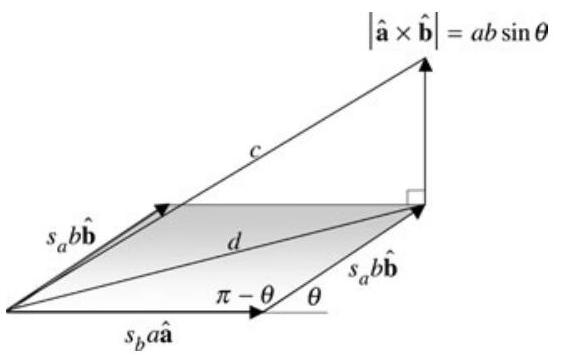
\includegraphics[max width=0.7\textwidth]{2023_01_16_a848224efad29cd66460g-079}
    \caption[short]{$s_{a} b \hat{\mathbf{b}}+s_{b} a \hat{\mathbf{a}}+a b \sin \theta(\hat{\mathbf{a}} \times \hat{\mathbf{b}})$几何表示}
\end{figure}

图$5.2$展示了c的几何图形表示。
$$
\begin{aligned}
d^{2}= & s_{b}^{2} a^{2}+s_{a}^{2} b^{2}-2 s_{a} s_{b} a b \cos (\pi-\theta) \\
= & s_{b}^{2} a^{2}+s_{a}^{2} b^{2}+2 s_{a} s_{b} a b \cos \theta \\
c^{2}= & d^{2}+a^{2} b^{2} \sin ^{2} \theta \\
= & s_{b}^{2} a^{2}+s_{a}^{2} b^{2}+2 s_{a} s_{b} a b \cos \theta+a^{2} b^{2} \sin ^{2} \theta \\
s_{c}^{2}+c^{2}= & s_{a}^{2} s_{b}^{2}-2 s_{a} s_{b} a b \cos \theta+a^{2} b^{2} \cos ^{2} \theta+s_{b}^{2} a^{2}+s_{a}^{2} b^{2}+2 s_{a} s_{b} a b \cos \theta \\
& +a^{2} b^{2} \sin ^{2} \theta \\
= & s_{a}^{2} s_{b}^{2}+a^{2} b^{2}+s_{b}^{2} a^{2}+s_{a}^{2} b^{2} \\
= & s_{a}^{2}\left(s_{b}^{2}+b^{2}\right)+a^{2}\left(s_{b}^{2}+b^{2}\right) \\
= & s_{a}^{2}+a^{2} \\
= & 1 .
\end{aligned}
$$

因此,两个单位范数四元数的乘积是另一个单位范数四元数。因此,用一个四元数乘以一个单位范数四元数并不改变它的范数:
$$
\begin{aligned}
q_{a} & =\left[s_{a}, \mathbf{a}\right] \\
\left|q_{a}\right| & =1 \\
q_{b} & =\left[s_{b}, \mathbf{b}\right] \\
\left|q_{a} q_{b}\right| & =\left|q_{b}\right| .
\end{aligned}
$$

\subsection{四元数平方}
四元数的平方由
$$
\begin{aligned}
q & =[s, \mathbf{v}] \\
q^{2} & =[s, \mathbf{v}][s, \mathbf{v}] \\
& =\left[s^{2}-\mathbf{v} \cdot \mathbf{v}, 2 s \mathbf{v}+\mathbf{v} \times \mathbf{v}\right] \\
& =\left[s^{2}-\mathbf{v} \cdot \mathbf{v}, 2 s \mathbf{v}\right] \\
& =\left[s^{2}-x^{2}-y^{2}-z^{2}, 2 s(x \mathbf{i}+y \mathbf{j}+z \mathbf{k})\right] .
\end{aligned}
$$

例如:
$$
\begin{aligned}
q & =[7,2 \mathbf{i}+3 \mathbf{j}+4 \mathbf{k}] \\
q^{2} & =\left[7^{2}-2^{2}-3^{2}-4^{2}, 14(2 \mathbf{i}+3 \mathbf{j}+4 \mathbf{k})\right] \\
& =[20,28 \mathbf{i}+42 \mathbf{j}+56 \mathbf{k}] .
\end{aligned}
$$

纯四元数的平方是
$$
\begin{aligned}
q & =[0, \mathbf{v}] \\
q^{2} & =[0, \mathbf{v}][0, \mathbf{v}] \\
& =[0-\mathbf{v} \cdot \mathbf{v}, \mathbf{v} \times \mathbf{v}] \\
& =[0-\mathbf{v} \cdot \mathbf{v}, \mathbf{0}] \\
& =\left[-\left(x^{2}+y^{2}+z^{2}\right), \mathbf{0}\right]
\end{aligned}
$$

这使得一个纯粹的单位范数四元数的平方等于$-1$,这是19世纪一些数学家反对的结果之一。

\subsection{四元数乘积的范数}
在证明两个单位范数四元数的乘积是另一个单位范数四元数时,我们看到了这一点
$$
\begin{aligned}
q_{a} & =\left[s_{a}, \mathbf{a}\right] \\
q_{b} & =\left[s_{b}, \mathbf{b}\right] \\
q_{c} & =q_{a} q_{b} \\
\left|q_{c}\right|^{2} & =s_{a}^{2}\left(s_{b}^{2}+b^{2}\right)+a^{2}\left(s_{b}^{2}+b^{2}\right) \\
& =\left(s_{a}^{2}+a^{2}\right)\left(s_{b}^{2}+b^{2}\right)
\end{aligned}
$$

如果我们忽略单位范数四元数的约束,则表明四元数乘积的范数等于各个范数的乘积:
$$
\begin{aligned}
\left|q_{a} q_{b}\right|^{2} & =\left|q_{a}\right|^{2}\left|q_{b}\right|^{2} \\
\left|q_{a} q_{b}\right| & =\left|q_{a}\right|\left|q_{b}\right|
\end{aligned}
$$

\section{逆四元数}
四元数代数的一个重要特征是能够两个四元数$q_{b} / q_{a}$相除,只要$q_{a}$不为$[0,\bf{0}]$。

根据定义,$q$的逆$q^{-1}$满足
\begin{align}
    q q^{-1}=[1, \mathbf{0}]=1
\end{align}

为了分离$q^{-1}$,我们将(5.12)乘以$q^{*}$
\begin{align}
    \begin{aligned}
        & q^{*} q q^{-1}=q^{*} \\
        & |q|^{2} q^{-1}=q^{*}
    \end{aligned}
\end{align}

从(5.13)我们可以写出
$$
q^{-1}=\frac{q^{*}}{|q|^{2}}
$$

如果$q$是单位范数四元数,则
$$
q^{-1}=q^{*}
$$

这在旋转的情况下很有用。

此外,由于
$$
\left(q_{a} q_{b}\right)^{*}=q_{b}^{*} q_{a}^{*}
$$

然后
$$
\left(q_{a} q_{b}\right)^{-1}=q_{b}^{-1} q_{a}^{-1}
$$

注意$q q^{-1}=q^{-1} q$
$$
\begin{aligned}
& q q^{-1}=\frac{q q^{*}}{|q|^{2}}=1 \\
& q^{-1} q=\frac{q^{*} q}{|q|^{2}}=1
\end{aligned}
$$

因此,我们将商$q_{b} / q_{a}$表示为
$$
\begin{aligned}
q_{c} & =\frac{q_{b}}{q_{a}} \\
& =q_{b} q_{a}^{-1} \\
& =\frac{q_{b} q_{a}^{*}}{\left|q_{a}\right|^{2}}
\end{aligned}
$$

为了完整,我们求$q$的逆
$$
\begin{aligned}
q & =\left[1, \frac{1}{\sqrt{3}} \mathbf{i}+\frac{1}{\sqrt{3}} \mathbf{j}+\frac{1}{\sqrt{3}} \mathbf{k}\right] \\
q^{*} & =\left[1,-\frac{1}{\sqrt{3}} \mathbf{i}-\frac{1}{\sqrt{3}} \mathbf{j}-\frac{1}{\sqrt{3}} \mathbf{k}\right] \\
|q|^{2} & =1+\frac{1}{3}+\frac{1}{3}+\frac{1}{3}=2 \\
q^{-1}=\frac{q^{*}}{|q|^{2}} & =\frac{1}{2}\left[1,-\frac{1}{\sqrt{3}} \mathbf{i}-\frac{1}{\sqrt{3}} \mathbf{j}-\frac{1}{\sqrt{3}} \mathbf{k}\right]
\end{aligned}
$$

显然$q^{-1} q=1$:
$$
\begin{aligned}
q^{-1} q & =\frac{1}{2}\left[1,-\frac{1}{\sqrt{3}} \mathbf{i}-\frac{1}{\sqrt{3}} \mathbf{j}-\frac{1}{\sqrt{3}} \mathbf{k}\right]\left[1, \frac{1}{\sqrt{3}} \mathbf{i}+\frac{1}{\sqrt{3}} \mathbf{j}+\frac{1}{\sqrt{3}} \mathbf{k}\right] \\
& =\frac{1}{2}\left[1+\frac{1}{3}+\frac{1}{3}+\frac{1}{3}, \mathbf{0}\right] \\
& =1 .
\end{aligned}
$$

\section{矩阵}
矩阵提供了另一种表示四元数积的方法。为方便起见,让我们再次重复式(5.8),并以矩阵形式表示:
$$
\begin{aligned}
{\left[s_{a}, \mathbf{a}\right]\left[s_{b}, \mathbf{b}\right]=} & {\left[s_{a} s_{b}-x_{a} x_{b}-y_{a} y_{b}-z_{a} z_{b},\right.} \\
& s_{a}\left(x_{b} \mathbf{i}+y_{b} \mathbf{j}+z_{b} \mathbf{k}\right)+s_{b}\left(x_{a} \mathbf{i}+y_{a} \mathbf{j}+z_{a} \mathbf{k}\right) \\
& \left.+\left(y_{a} z_{b}-y_{b} z_{a}\right) \mathbf{i}+\left(z_{a} x_{b}-z_{b} x_{a}\right) \mathbf{j}+\left(x_{a} y_{b}-x_{b} y_{a}\right) \mathbf{k}\right] \\
= & {\left[\begin{array}{cccc}
s_{a} & -x_{a} & -y_{a} & -z_{a} \\
x_{a} & s_{a} & -z_{a} & y_{a} \\
y_{a} & z_{a} & s_{a} & -x_{a} \\
z_{a} & -y_{a} & x_{a} & s_{a}
\end{array}\right]\left[\begin{array}{c}
s_{b} \\
x_{b} \\
y_{b} \\
z_{b}
\end{array}\right] . }
\end{aligned}
$$

让我们用上面的矩阵重新计算乘积$q_{a} q_{b}$:
$$
\begin{aligned}
q_{a} & =[1,2 \mathbf{i}+3 \mathbf{j}+4 \mathbf{k}] \\
q_{b} & =[2,3 \mathbf{i}+4 \mathbf{j}+5 \mathbf{k}] \\
q_{a} q_{b} & =\left[\begin{array}{cccc}
1 & -2 & -3 & -4 \\
2 & 1 & -4 & 3 \\
3 & 4 & 1 & -2 \\
4 & -3 & 2 & 1
\end{array}\right]\left[\begin{array}{l}
2 \\
3 \\
4 \\
5
\end{array}\right] \\
& =\left[\begin{array}{c}
-36 \\
6 \\
12 \\
12
\end{array}\right] \\
& =[-36,6 \mathbf{i}+12 \mathbf{j}+12 \mathbf{k}] .
\end{aligned}
$$

\subsection{正交矩阵}
我们可以证明单位范数四元数矩阵是正交的,通过证明其转置的乘积等于单位矩阵。当我们处理矩阵时,$\mathbf{Q}$将表示 $ q $ 的矩阵:

$$
\begin{aligned}
& q=[s, x \mathbf{i}+y \mathbf{j}+z \mathbf{k}] \quad \text { where } 1=s^{2}+x^{2}+y^{2}+z^{2} \\
& \mathbf{Q}=\left[\begin{array}{cccc}s & -x & -y & -z \\x & s & -z & y \\y & z & s & -x \\z & -y & x & s\end{array}\right] \\
& \mathbf{Q}^{\mathrm{T}}=\left[\begin{array}{cccc}s & x & y & z \\-x & s & z & -y \\-y & -z & s & x \\-z & y & -x & s\end{array}\right] \\
& \mathbf{Q} \mathbf{Q}^{\mathrm{T}}=\left[\begin{array}{cccc}s & -x & -y & -z \\x & s & -z & y \\y & z & s & -x \\z & -y & x & s\end{array}\right]\left[\begin{array}{cccc}s & x & y & z \\-x & s & z & -y \\-y & -z & s & x \\-z & y & -x & s\end{array}\right] \\
& =\left[\begin{array}{llll}1 & 0 & 0 & 0 \\0 & 1 & 0 & 0 \\0 & 0 & 1 & 0 \\0 & 0 & 0 & 1\end{array}\right] \text {. }
\end{aligned}
$$

会发生这样的情况, $\mathbf{Q}^{\mathrm{T}}=\mathbf{Q}^{-1}$。

\section{四元数代数}
有序对提供了一种简单的表示四元数的表示法,并允许我们将实单位1表示为$[1,\mathbf{0}]$,将虚数$i, j, k$分别表示为$[0, \mathbf{i}],[0, \mathbf{j}],[0, \mathbf{k}]$。四元数就变成了这些元素的线性组合,并带有相关的实系数。在这种情况下,这些元素构成了实数域代数的基础。

此外,由于四元数代数支持除法,并且遵循代数的正常公理,除了乘法是非交换的,所以它被称为除法代数。Ferdinand Georg Frobenius在1878年证明了只有三种实数结合律除法代数存在:实数,复数和四元数[1]。

“Cayley数”$\mathbb{O}$,构成了一个实除法代数,但Cayley数是8维的,并且是不符合结合律的,即$a(b c) \neq(a b) c$对于所有$a, b, c \in \mathbb{O}$。

\section{总结}
四元数与复数非常相似,除了它们有三个虚数项,而不是一个。因此,它们继承了与复数相关的一些性质,如模、共轭、单位模和逆。它们还可以加、减、乘、除。然而,与复数不同的是,它们在相乘时是不符合交换律的。

\subsection{操作符总结}
\subsubsection*{四元数}
$$
\begin{aligned}
q_{a} & =\left[s_{a}, \mathbf{a}\right]=\left[s_{a}, x_{a} \mathbf{i}+y_{a} \mathbf{j}+z_{a} \mathbf{k}\right] \\
q_{b} & =\left[s_{b}, \mathbf{b}\right]=\left[s_{b}, x_{b} \mathbf{i}+y_{b} \mathbf{j}+z_{b} \mathbf{k}\right]
\end{aligned}
$$

\subsubsection*{加减法}
$$
q_{a} \pm q_{b}=\left[s_{a} \pm s_{b}, \mathbf{a} \pm \mathbf{b}\right]
$$

\subsubsection*{乘积}
$$
\begin{aligned}
q_{a} q_{b} & =\left[s_{a}, \mathbf{a}\right]\left[s_{b}, \mathbf{b}\right] \\
& =\left[s_{a} s_{b}-\mathbf{a} \cdot \mathbf{b}, s_{a} \mathbf{b}+s_{b} \mathbf{a}+\mathbf{a} \times \mathbf{b}\right] \\
& =\left[\begin{array}{cccc}
s_{a} & -x_{a} & -y_{a} & -z_{a} \\
x_{a} & s_{a} & -z_{a} & y_{a} \\
y_{a} & z_{a} & s_{a} & -x_{a} \\
z_{a} & -y_{a} & x_{a} & s_{a}
\end{array}\right]\left[\begin{array}{c}
s_{b} \\
x_{b} \\
y_{b} \\
z_{b}
\end{array}\right]
\end{aligned}
$$

\subsubsection*{平方}
$$
\begin{aligned}
q^{2} & =[s, \mathbf{v}][s, \mathbf{v}] \\
& =\left[s^{2}-x^{2}-y^{2}-z^{2}, 2 s(x \mathbf{i}+y \mathbf{j}+z \mathbf{k})\right]
\end{aligned}
$$

\subsubsection*{纯}
$$
\begin{aligned}
q^{2} & =[0, \mathbf{v}][0, \mathbf{v}] \\
& =\left[-\left(x^{2}+y^{2}+z^{2}\right), \mathbf{0}\right]
\end{aligned}
$$

\subsubsection*{范数}
$$
|q|=\sqrt{s^{2}+v^{2}}
$$

\subsubsection*{单位范数}
$$
|q|=\sqrt{s^{2}+v^{2}}=1
$$

\subsubsection*{共轭}
$$
\begin{aligned}
q^{*} & =[s,-\mathbf{v}] \\
\left(q_{a} q_{b}\right)^{*} & =q_{b}^{*} q_{a}^{*}
\end{aligned}
$$

\subsubsection*{逆}
$$
\begin{aligned}
q^{-1} & =\frac{q^{*}}{|q|^{2}} \\
\left(q_{a} q_{b}\right)^{-1} & =q_{b}^{-1} q_{a}^{-1}
\end{aligned}
$$

\section{样例}
下面是一些进一步使用上述思想的示例。在某些情况下,包括测试来确认结果。

例1 加减以下四元数:
$$
\begin{aligned}
q_{a} & =[2,-2 \mathbf{i}+3 \mathbf{j}-4 \mathbf{k}] \\
q_{b} & =[1,-2 \mathbf{i}+5 \mathbf{j}-6 \mathbf{k}] \\
q_{a}+q_{b} & =[3,-4 \mathbf{i}+8 \mathbf{j}-10 \mathbf{k}] \\
q_{a}-q_{b} & =[1,-2 \mathbf{j}+2 \mathbf{k}] .
\end{aligned}
$$

例2 求下列四元数的范数:
$$
\begin{aligned}
q_{a} & =[2,-2 \mathbf{i}+3 \mathbf{j}-4 \mathbf{k}] \\
q_{b} & =[1,-2 \mathbf{i}+5 \mathbf{j}-6 \mathbf{k}] \\
\left|q_{a}\right| & =\sqrt{2^{2}+(-2)^{2}+3^{2}+(-4)^{2}}=\sqrt{33} \\
\left|q_{b}\right| & =\sqrt{1^{2}+(-2)^{2}+5^{2}+(-6)^{2}}=\sqrt{66} .
\end{aligned}
$$

例3 将这些四元数转换为它们的单位范数形式:
$$
\begin{aligned}
q_{a} & =[2,-2 \mathbf{i}+3 \mathbf{j}-4 \mathbf{k}] \\
q_{b} & =[1,-2 \mathbf{i}+5 \mathbf{j}-6 \mathbf{k}] \\
\left|q_{a}\right| & =\sqrt{33} \\
\left|q_{b}\right| & =\sqrt{66} \\
q_{a}^{\prime} & =\frac{1}{\sqrt{33}}[2,-2 \mathbf{i}+3 \mathbf{j}-4 \mathbf{k}] \\
q_{b}^{\prime} & =\frac{1}{\sqrt{66}}[1,-2 \mathbf{i}+5 \mathbf{j}-6 \mathbf{k}] .
\end{aligned}
$$

例4 计算以下四元数的乘积和反向乘积。
$$
\begin{aligned}
q_{a}= & {[2,-2 \mathbf{i}+3 \mathbf{j}-4 \mathbf{k}] } \\
q_{b}= & {[1,-2 \mathbf{i}+5 \mathbf{j}-6 \mathbf{k}] } \\
q_{a} q_{b}= & {[2,-2 \mathbf{i}+3 \mathbf{j}-4 \mathbf{k}][1,-2 \mathbf{i}+5 \mathbf{j}-6 \mathbf{k}] } \\
= & {[2 \times 1-((-2) \times(-2)+3 \times 5+(-4) \times(-6)),} \\
& 2(-2 \mathbf{i}+5 \mathbf{j}-6 \mathbf{k})+1(-2 \mathbf{i}+3 \mathbf{j}-4 \mathbf{k}) \\
& +(3 \times(-6)-(-4) \times 5) \mathbf{i}-((-2) \times(-6)-(-4) \times(-2)) \mathbf{j} \\
& +((-2) \times 5-3 \times(-2)) \mathbf{k}] \\
= & {[-41,-6 \mathbf{i}+13 \mathbf{j}-16 \mathbf{k}+2 \mathbf{i}-4 \mathbf{j}-4 \mathbf{k}] } \\
= & {[-41,-4 \mathbf{i}+9 \mathbf{j}-20 \mathbf{k}] }\\
q_{b} q_{a}= & {[1,-2 \mathbf{i}+5 \mathbf{j}-6 \mathbf{k}][2-2 \mathbf{i}+3 \mathbf{j}-4 \mathbf{k}] } \\
= & {[1 \times 2-((-2) \times(-2)+5 \times 3+(-6) \times(-4)),} \\
& 1(-2 \mathbf{i}+3 \mathbf{j}-4 \mathbf{k})+2(-2 \mathbf{i}+5 \mathbf{j}-6 \mathbf{k}) \\
& +(5 \times(-4)-(-6) \times 3) \mathbf{i}-((-2) \times(-4)-(-6) \times(-2)) \mathbf{j} \\
& +((-2) \times 3-5 \times(-2)) \mathbf{k}] \\
= & {[-41,-6 \mathbf{i}+13 \mathbf{j}-16 \mathbf{k}-2 \mathbf{i}+4 \mathbf{j}+4 \mathbf{k}] } \\
= & {[-41,-8 \mathbf{i}+17 \mathbf{j}-12 \mathbf{k}] }
\end{aligned}
$$

注意:在这个计算中唯一改变的是轴向量叉乘的符号。

例5 计算这个四元数的平方:
$$
\begin{aligned}
q= & {[2,-2 \mathbf{i}+3 \mathbf{j}-4 \mathbf{k}] } \\
q^{2}= & {[2,-2 \mathbf{i}+3 \mathbf{j}-4 \mathbf{k}][2,-2 \mathbf{i}+3 \mathbf{j}-4 \mathbf{k}] } \\
= & {[2 \times 2-((-2) \times(-2)+3 \times 3+(-4) \times(-4))} \\
& 2 \times 2(-2 \mathbf{i}+3 \mathbf{j}-4 \mathbf{k})] \\
= & {[-25,-8 \mathbf{i}+12 \mathbf{j}-16 \mathbf{k}] }
\end{aligned}
$$

例6 计算这个四元数的逆:

$$
\begin{aligned}
q & =[2,-2 \mathbf{i}+3 \mathbf{j}-4 \mathbf{k}] \\
q^{*} & =[2,+2 \mathbf{i}-3 \mathbf{j}+4 \mathbf{k}] \\
|q|^{2} & =2^{2}+(-2)^{2}+3^{2}+(-4)^{2}=33 \\
q^{-1} & =\frac{1}{33}[2,2 \mathbf{i}-3 \mathbf{j}+4 \mathbf{k}] .
\end{aligned}
$$

\chap{3D旋转变换}
\section{介绍}
在本章中,我们回顾了在计算机图形软件中使用的三维欧拉旋转变换。特别地,我们确定了他们的阿喀琉斯之踵——万向节锁——以及能够围绕任意轴旋转的需求。为此,我们将开发一个实现这种旋转的矩阵变换,并在下一章中使用四元数开发一个类似的变换。

\section{3D旋转变换}
旋转点和参考系的传统技术是基于欧拉旋转,以瑞士数学家Leonhard Euler的名字命名。他们提供了三种轮换的方法。第一种是绕三个笛卡尔轴之一旋转。第二个组合了任意两个围绕不同轴的旋转,第三个组合了任意三个旋转。

最初,这种方法听起来很吸引人——在许多情况下效果很好,然而,这种技术存在一些问题。第一个问题是,当两个或多个旋转结合在一起时,很难可视化和预测最终的旋转将如何表现。第二点是,绕一个特定的轴旋转是很复杂的,第三点是,在某些条件下,人们失去了对物体的一个旋转轴的访问。最后一个问题被称为万向节锁。为了理解这些问题,我们将构建一个受万向节锁定影响的三维旋转变换。

\section{绕笛卡尔轴旋转}
一个点在平面上绕原点旋转的变换由
$$
\mathbf{R}_{\beta}=\left[\begin{array}{cc}
\cos \beta & -\sin \beta \\
\sin \beta & \cos \beta
\end{array}\right] .
$$

这可以通过添加第三个坐标推广到围绕笛卡尔轴的三维旋转。例如,要绕$z$-轴旋转,我们添加一个$z$-坐标,如下所示:
$$
\mathbf{R}_{\beta, z}=\left[\begin{array}{ccc}
\cos \beta & -\sin \beta & 0 \\
\sin \beta & \cos \beta & 0 \\
0 & 0 & 1
\end{array}\right]
$$

\begin{figure}[h!]
    \centering
    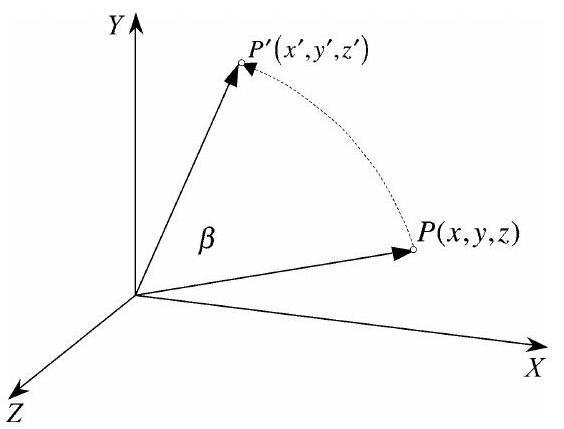
\includegraphics[max width=0.5\textwidth]{2023_01_16_a848224efad29cd66460g-089}
    \caption[short]{点 $P$ 围绕 $z$ 轴旋转}
\end{figure}

如图6.1所示。要围绕$x$-轴旋转一个点,$x$-坐标保持不变,而$y$ -和$z$-坐标根据$2 \mathrm{D}$旋转变换进行更改:
$$
\mathbf{R}_{\beta, x}=\left[\begin{array}{ccc}
1 & 0 & 0 \\
0 & \cos \beta & -\sin \beta \\
0 & \sin \beta & \cos \beta
\end{array}\right] .
$$

最后,为了绕$y$-轴旋转,$y$-坐标保持不变,而$x$和$z$-坐标改变:
$$
\mathbf{R}_{\beta, y}=\left[\begin{array}{ccc}
\cos \beta & 0 & \sin \beta \\
0 & 1 & 0 \\
-\sin \beta & 0 & \cos \beta
\end{array}\right] .
$$

\section{绕偏移轴旋转}
要绕与笛卡尔轴之一平行的轴旋转,通常采用齐次坐标并平移要旋转的点,这样它可以绕原点旋转,然后平移回来一个相等且相反的量。假定读者熟悉这种策略。但是,为了完整起见,我们将构造一个变换,使一个点围绕一个与$z$-轴平行的轴旋转,并与点$\left(t_{x}, t_{y}, 0\right)$相交,如图6.2所示:
$$
\left[\begin{array}{c}
x^{\prime} \\
y^{\prime} \\
z^{\prime} \\
1
\end{array}\right]=\mathbf{T}_{t_{x}, t_{y}, 0} \mathbf{R}_{\beta, z} \mathbf{T}_{-t_{x},-t_{y}, 0}\left[\begin{array}{c}
x \\
y \\
z \\
1
\end{array}\right]
$$

\begin{figure}
    \centering
    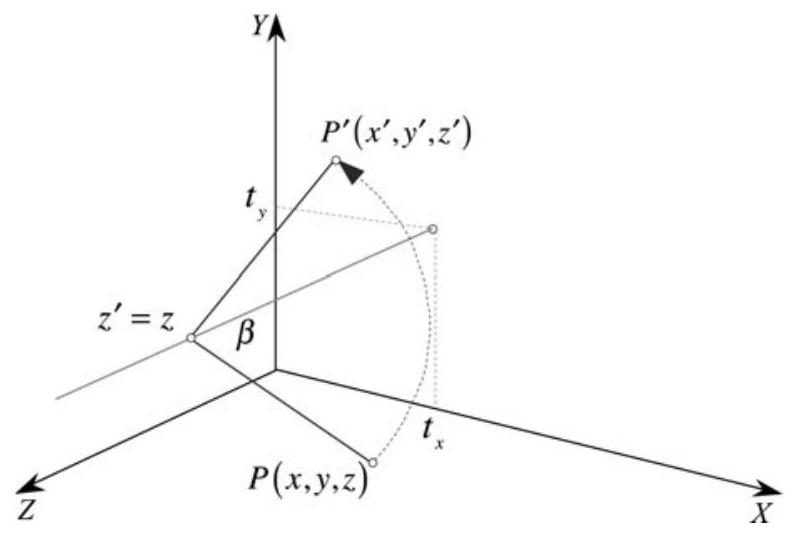
\includegraphics[max width=0.6\textwidth]{2023_01_16_a848224efad29cd66460g-090}
    \caption[short]{绕平行于$z$-轴的轴旋转一点}
\end{figure}

其中
$$
\begin{aligned}
& \mathbf{T}_{-t_{x},-t_{y}, 0} && \text { 创建临时原点 } \\
& \mathbf{R}_{\beta, z} && \text { 围绕临时的 } z \text {轴旋转 }\beta \text{角度} \\
& \mathbf{T}_{t_{x}, t_{y}, 0} && \text { 回到原来的坐标系中的位置 }
\end{aligned}
$$

矩阵变换是
$$
\mathbf{R}_{\beta, z,\left(t_{x}, t_{y}, 0\right)}=\left[\begin{array}{cccc}
\cos \beta & -\sin \beta & 0 & t_{x}(1-\cos \beta)+t_{y} \sin \beta \\
\sin \beta & \cos \beta & 0 & t_{y}(1-\cos \beta)-t_{x} \sin \beta \\
0 & 0 & 1 & 0 \\
0 & 0 & 0 & 1
\end{array}\right]
$$

围绕平行于$x$-轴和平行于$y$-轴的偏移轴旋转的矩阵为:
$$
\begin{aligned}
\mathbf{R}_{\beta, x,\left(0, t_{y}, t_{z}\right)} & =\left[\begin{array}{cccc}
1 & 0 & 0 & 0 \\
0 & \cos \beta & -\sin \beta & t_{y}(1-\cos \beta)+t_{z} \sin \beta \\
0 & \sin \beta & \cos \beta & t_{z}(1-\cos \beta)-t_{y} \sin \beta \\
0 & 0 & 0 & 1
\end{array}\right] \\
\mathbf{R}_{\beta, y,\left(t_{x}, 0, t_{z}\right)} & =\left[\begin{array}{cccc}
\cos \beta & 0 & \sin \beta & t_{x}(1-\cos \beta)-t_{z} \sin \beta \\
0 & 1 & 0 & 0 \\
-\sin \beta & 0 & \cos \beta & t_{z}(1-\cos \beta)+t_{x} \sin \beta \\
0 & 0 & 0 & 1
\end{array}\right] .
\end{aligned}
$$

\section{复合旋转}
撇开围绕单轴和偏移轴旋转的变换不谈,我们有三个围绕笛卡尔轴旋转的变换:$\mathbf{R}_{\alpha, x}, \mathbf{R}_{\beta, y}$和$\mathbf{R}_{\gamma, z}$,它们可以组合成双变换族和三重变换族。如上所述,这种旋转称为欧拉旋转,假定读者熟悉其结构。三重变换族是:
$$
\begin{array}{llll}
\mathbf{R}_{\gamma, x} \mathbf{R}_{\beta, y} \mathbf{R}_{\alpha, x} & \mathbf{R}_{\gamma, x} \mathbf{R}_{\beta, y} \mathbf{R}_{\alpha, z} & \mathbf{R}_{\gamma, x} \mathbf{R}_{\beta, z} \mathbf{R}_{\alpha, x} & \mathbf{R}_{\gamma, x} \mathbf{R}_{\beta, z} \mathbf{R}_{\alpha, y} \\
\mathbf{R}_{\gamma, y} \mathbf{R}_{\beta, x} \mathbf{R}_{\alpha, y} & \mathbf{R}_{\gamma, y} \mathbf{R}_{\beta, x} \mathbf{R}_{\alpha, z} & \mathbf{R}_{\gamma, y} \mathbf{R}_{\beta, z} \mathbf{R}_{\alpha, x} & \mathbf{R}_{\gamma, y} \mathbf{R}_{\beta, z} \mathbf{R}_{\alpha, y} \\
\mathbf{R}_{\gamma, z} \mathbf{R}_{\beta, x} \mathbf{R}_{\alpha, y} & \mathbf{R}_{\gamma, z} \mathbf{R}_{\beta, x} \mathbf{R}_{\alpha, z} & \mathbf{R}_{\gamma, z} \mathbf{R}_{\beta, y} \mathbf{R}_{\alpha, x} & \mathbf{R}_{\gamma, z} \mathbf{R}_{\beta, y} \mathbf{R}_{\alpha, z} .
\end{array}
$$

为了说明万向节锁的问题,我们将使用一个立方体,其顶点编号为0到7,如图6.3所示。
\begin{figure}[h!]
    \centering
    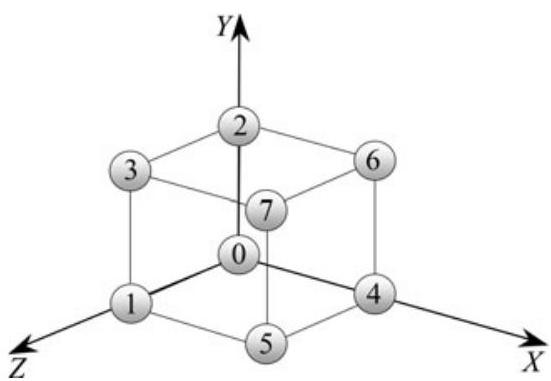
\includegraphics[max width=0.4\textwidth]{2023_01_16_a848224efad29cd66460g-091}
    \caption[short]{位于原点的单位立方体}
\end{figure}

\begin{figure}[h!]
    \centering
    \subfigure[]{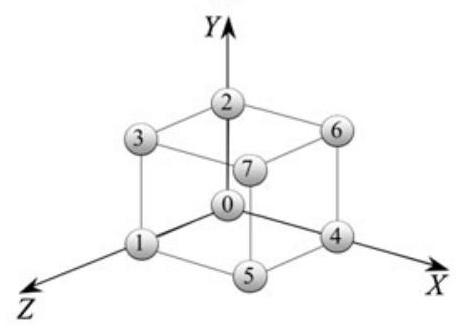
\includegraphics[max width=0.35\textwidth]{2023_01_16_a848224efad29cd66460g-091(1)}}
    \subfigure[]{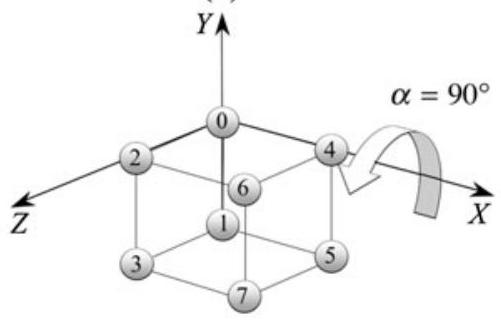
\includegraphics[max width=0.35\textwidth]{2023_01_16_a848224efad29cd66460g-091(3)}}\\
    \subfigure[]{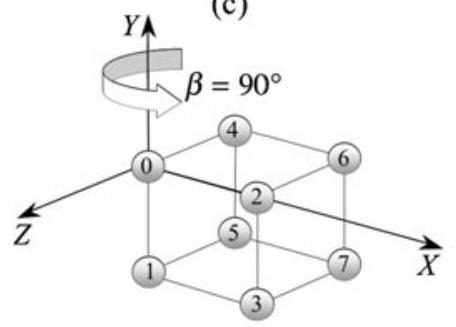
\includegraphics[max width=0.35\textwidth]{2023_01_16_a848224efad29cd66460g-091(2)}}
    \subfigure[]{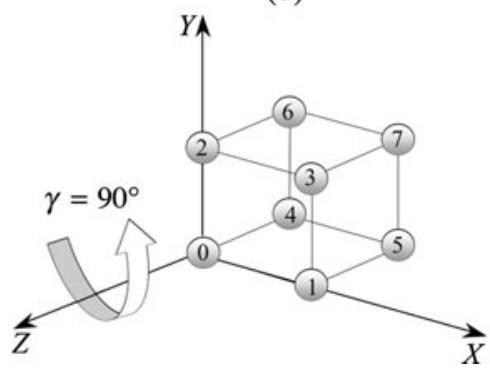
\includegraphics[max width=0.35\textwidth]{2023_01_16_a848224efad29cd66460g-091(4)}}
    \caption[short]{单位立方体在三次旋转之前和期间的四个视图}
\end{figure}

我们可以通过在任意序列中放置$\mathbf{R}_{\alpha, x}, \mathbf{R}_{\beta, y}$和$\mathbf{R}_{\gamma, z}$来创建复合旋转变换——甚至可以重复其中一个序列两次,只要它们被不同的变换隔开。作为后者的一个例子,我们可以使用序列$\mathbf{R}_{\alpha, z} \mathbf{R}_{\beta, y} \mathbf{R}_{\gamma, z}$,其中我们围绕$z$-轴旋转两次。然而,为了说明万向节锁,让我们选择序列$\mathbf{R}_{\gamma, z} \mathbf{R}_{\beta, y} \mathbf{R}_{\alpha, x}$,并使$\alpha=\beta=\gamma=90^{\circ}$,这相当于围绕固定的$x$-轴旋转一个点$90^{\circ}$,然后围绕固定的$y$-轴旋转$90^{\circ}$,然后围绕固定的$z$-轴旋转$90^{\circ}$。该旋转序列如图6.4所示。

\begin{figure}[h!]
    \centering
    \subfigure[]{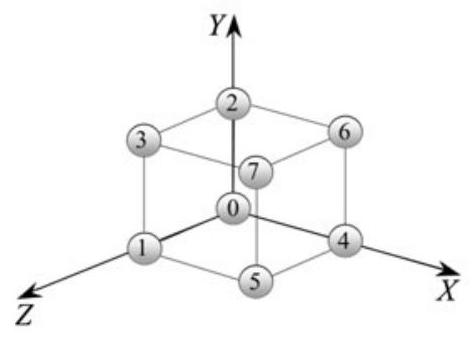
\includegraphics[max width=0.35\textwidth]{2023_01_16_a848224efad29cd66460g-092}}
    \subfigure[]{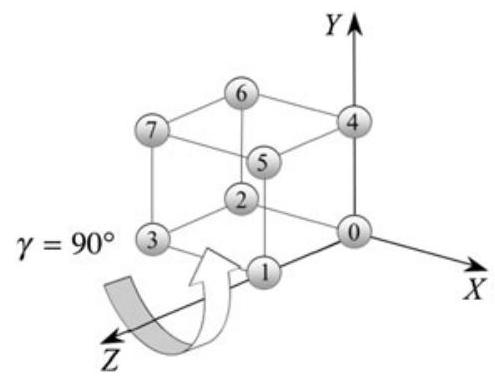
\includegraphics[max width=0.35\textwidth]{2023_01_16_a848224efad29cd66460g-092(2)}}\\
    \subfigure[]{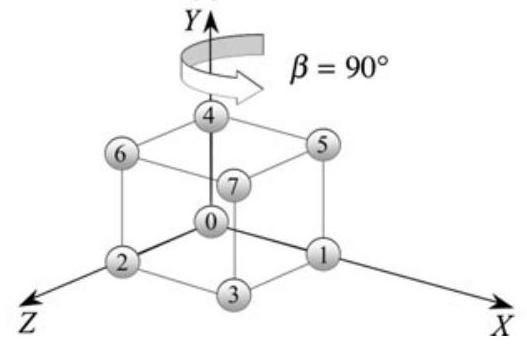
\includegraphics[max width=0.35\textwidth]{2023_01_16_a848224efad29cd66460g-092(1)}}
    \subfigure[]{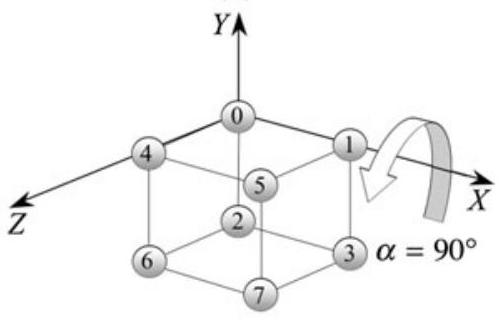
\includegraphics[max width=0.35\textwidth]{2023_01_16_a848224efad29cd66460g-092(3)}}
    \caption[short]{使用旋转序列$\mathbf{R}_{\alpha, x} \mathbf{R}_{\beta, y} \mathbf{R}_{\gamma, z}$的单位立方体的四个视图}
\end{figure}

图$6.4$ (a)显示了立方体的起始位置;(b)在绕$x$轴旋转$90^{\circ}$后显示其位置;(c)在绕$y$轴进一步旋转$90^{\circ}$后显示其位置;(d)立方体绕z轴旋转$90^{\circ}$后的静止位置。

然而,尽管采用了围绕不同轴的三次旋转,立方体实际上只围绕$y$轴旋转了$90^{\circ}$!立方体绕着穿过顶点0和4的轴旋转了两次,绕着穿过顶点0和1的轴旋转了一次,但是穿过顶点0和2的轴被忽略了。这被称为万向节锁定,并通过一个不幸的旋转序列组合和角度而产生。

将复合旋转反转到$\mathbf{R}_{\alpha, x} \mathbf{R}_{\beta, y} \mathbf{R}_{\gamma, z}$并不能改善问题。这个复合变换等价于围绕固定的z轴旋转一个点$90^{\circ}$,然后围绕固定的$y$-轴旋转$90^{\circ}$,然后围绕固定的$x$-轴旋转$90^{\circ}$。该旋转序列如图6.5所示。

对图$6.5$ (d)的检查显示,单位立方体已经围绕向量$\left[\begin{array}{lll}1 & 0 & 1\end{array}\right]^{\mathrm{T}}$旋转了$180^{\circ}$,即一个与顶点0和5相交的轴。这一次,立方体围绕与顶点0和1相交的轴旋转了两次,围绕与顶点0和4相交的轴旋转了一次,同样,与顶点0和2相交的轴被忽略了。不难看出为什么欧拉旋转会引起这么多问题。让我们继续,看看如何绕任意轴旋转。



\section{绕任意轴旋转}
单个欧拉变换并没有本质上的问题,问题是它们组合在一起产生旋转的方式有缺陷。理想情况下,我们需要一个旋转变换,允许我们指定轴和旋转角度,这是我们要计算的。第一种方法使用矩阵和三角函数,相当费力。第二种方法采用矢量分析,非常简洁。

\subsection{矩阵}
我们首先使用单位向量$\hat{\mathbf{n}}$定义一个轴,其中一个点$P$被旋转到$P^{\prime}$,如图6.6所示。由于我们只能使用围绕笛卡尔轴旋转点的矩阵,所以这个单位向量必须暂时与笛卡尔轴对齐。在下面的例子中,我们选择$x$-轴。在对齐过程中,点$P$进行必要的转换,以使单位向量与$x$-轴对齐。然后我们绕$x$轴旋转$P$。为了完成该操作,旋转后的点进行变换,使单位向量返回到其原始坐标系位置。

\begin{figure}[h!]
    \centering
    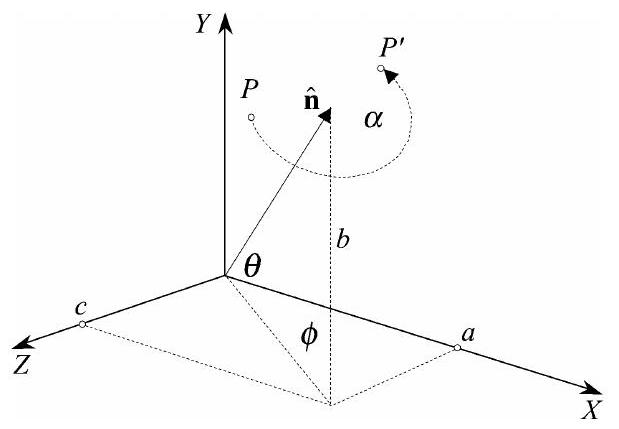
\includegraphics[max width=0.5\textwidth]{2023_01_16_a848224efad29cd66460g-093}
    \caption[short]{绕任意轴旋转的几何图形}
\end{figure}

虽然矩阵为这类工作提供了强大的工具,但它非常乏味,但却是提高一个人代数技能的好练习!

图$6.6$显示了一个点$P(x, y, z)$围绕如下定义的轴旋转一个角度$\alpha$到$\alpha$ to $P^{\prime}\left(x^{\prime}, y^{\prime}, z^{\prime}\right)$ 
$$
\hat{\mathbf{n}}=a \mathbf{i}+b \mathbf{j}+c \mathbf{k} .
$$

实现该操作的转换表达式如下:
$$
\left[\begin{array}{c}
x^{\prime} \\
y^{\prime} \\
z^{\prime}
\end{array}\right]=\mathbf{R}_{-\phi, y} \mathbf{R}_{\theta, z} \mathbf{R}_{\alpha, x} \mathbf{R}_{-\theta, z} \mathbf{R}_{\phi, y}\left[\begin{array}{c}
x \\
y \\
z
\end{array}\right]
$$

它将旋转轴与$x$-轴对齐,执行$P$的旋转,通过一个角度$\alpha$关于$x$-轴,并将旋转轴返回到其原始坐标系位置。因此,

$$
\begin{aligned}
\mathbf{R}_{\phi, y}= & {\left[\begin{array}{ccc}
\cos \phi & 0 & \sin \phi \\
0 & 1 & 0 \\
-\sin \phi & 0 & \cos \phi
\end{array}\right] } \\
\mathbf{R}_{\alpha, x}= & {\left[\begin{array}{ccc}
1 & 0 & 0 \\
0 & \cos \alpha & -\sin \alpha \\
0 & \sin \alpha & \cos \alpha
\end{array}\right] \mathbf{R}_{-\theta, z}=\left[\begin{array}{ccc}
\cos \theta & \sin \theta & 0 \\
-\sin \theta & \cos \theta & 0 \\
0 & 0 & 1
\end{array}\right] } \\
\mathbf{R}_{-\phi, y}= & {\left[\begin{array}{ccc}
\cos \phi & 0 & -\sin \phi \\
0 & 1 & 0 \\
\sin \phi & 0 & \cos \phi
\end{array}\right] }
\end{aligned}
$$

令
$$
\mathbf{R}_{-\phi, y} \mathbf{R}_{\theta, z} \mathbf{R}_{\alpha, x} \mathbf{R}_{-\theta, z} \mathbf{R}_{\phi, y}=\left[\begin{array}{lll}
a_{11} & a_{12} & a_{13} \\
a_{21} & a_{22} & a_{23} \\
a_{31} & a_{32} & a_{33}
\end{array}\right]
$$

其中,通过将矩阵相乘,我们发现:
$$
\begin{aligned}
a_{11}= & \cos ^{2} \phi \cos ^{2} \theta+\cos ^{2} \phi \sin ^{2} \theta \cos \alpha+\sin ^{2} \phi \cos \alpha \\
a_{12}= & \cos \phi \cos \theta \sin \theta-\cos \phi \sin \theta \cos \theta \cos \alpha-\sin \phi \cos \theta \sin \alpha \\
a_{13}= & \cos \phi \sin \phi \cos ^{2} \theta+\cos \phi \sin \phi \sin ^{2} \theta \cos \alpha+\sin ^{2} \phi \sin \theta \sin \alpha \\
& +\cos ^{2} \phi \sin \theta \sin \alpha-\cos \phi \sin \phi \cos \alpha \\
a_{21}= & \sin \theta \cos \theta \cos \phi-\cos \theta \sin \theta \cos \phi \cos \alpha+\cos \theta \sin \phi \sin \alpha \\
a_{22}= & \sin ^{2} \theta+\cos ^{2} \theta \cos \alpha \\
a_{23}= & \sin \theta \cos \theta \sin \phi-\cos \theta \sin \theta \sin \phi \cos \alpha-\cos \theta \cos \phi \sin \alpha \\
a_{31}= & \cos \phi \sin \phi \cos ^{2} \theta+\cos \phi \sin \phi \sin ^{2} \theta \cos \alpha-\cos 2 \phi \sin \theta \sin \alpha \\
= & -\cos \phi \sin \phi \cos \alpha \\
a_{32}= & \sin \phi \cos \theta \sin \theta-\sin \phi \sin ^{2} \theta \cos ^{2} \theta \cos \alpha+\cos \phi \cos \theta \sin \alpha \\
a_{33}= & \sin ^{2} \phi \cos \theta+\sin ^{2} \phi \sin ^{2} \theta \cos ^{2} \alpha-\cos \phi \sin \phi \sin \theta \sin \alpha \\
& +\cos \phi \sin \phi \sin \theta \sin \alpha+\cos ^{2} \phi \cos \alpha .
\end{aligned}
$$

经过大量的三角替换,我们得到了变换
$$
\left[\begin{array}{c}
x_{p}^{\prime} \\
y_{p}^{\prime} \\
z_{p}^{\prime}
\end{array}\right]=\left[\begin{array}{ccc}
a^{2} K+\cos \alpha & a b K-c \sin \alpha & a c K+b \sin \alpha \\
a b K+c \sin \alpha & b^{2} K+\cos \alpha & b c K-a \sin \alpha \\
a c K-b \sin \alpha & b c K+a \sin \alpha & c^{2} K+\cos \alpha
\end{array}\right]\left[\begin{array}{l}
x_{p} \\
y_{p} \\
z_{p}
\end{array}\right]
$$

其中
$$
K=1-\cos \alpha .
$$






\subsection{向量}
现在我们用向量来解决同样的问题。图$6.7$显示了与手头任务相关的几何视图。为了说明,图6.8显示了几何图形的横截面和平面图。

旋转轴由单位向量给出
$$
\hat{\mathbf{n}}=a \mathbf{i}+b \mathbf{j}+c \mathbf{k} .
$$
$P\left(x_{p}, y_{p}, z_{p}\right)$是将旋转$\alpha$角度到$P^{\prime}\left(x_{P}^{\prime}, y_{P}^{\prime}, z_{P}^{\prime}\right)$的点。

$O$是原点,$\mathbf{p}$和$\mathbf{p}^{\prime}$分别是$ P $和$ P ^{\prime}$的位置向量。
\begin{figure}[h!]
    \centering
    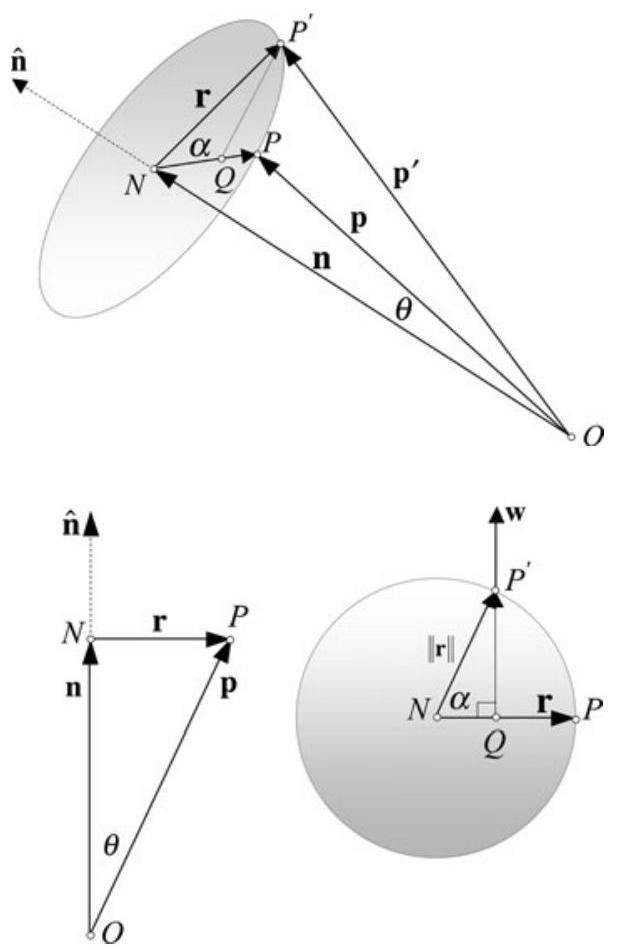
\includegraphics[max width=0.5\textwidth, center]{2023_01_16_a848224efad29cd66460g-095}
    \caption[short]{围绕任意轴旋转一点的几何学视图}
\end{figure}
\begin{figure}[h!]
    \centering
    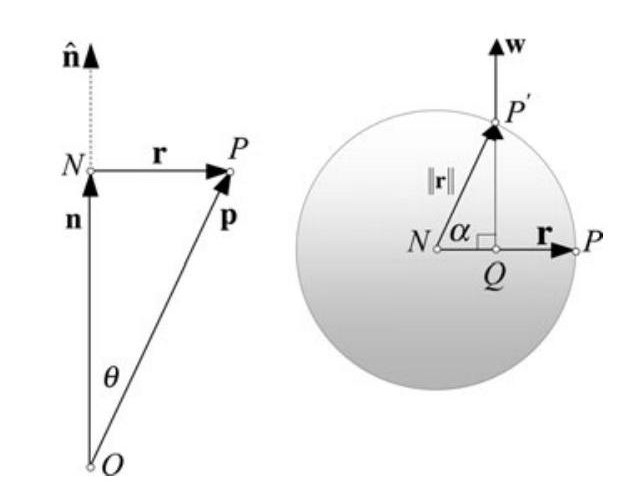
\includegraphics[max width=0.5\textwidth, center]{2023_01_16_a848224efad29cd66460g-095(1)}
    \caption[short]{绕任意轴旋转一点的几何学的横截面和平面视图}
\end{figure}

由图$6.7$和$6.8$:
$$
\mathbf{p}^{\prime}=\overrightarrow{O N}+\overrightarrow{N Q}+\overrightarrow{Q P^{\prime}}
$$

求 $\overrightarrow{O N}$
$$
|\mathbf{n}|=|\mathbf{p}| \cos \theta=\hat{\mathbf{n}} \cdot \mathbf{p}
$$

因此,
$$
\overrightarrow{O N}=\mathbf{n}=\hat{\mathbf{n}}(\hat{\mathbf{n}} \cdot \mathbf{p})
$$

求$\overrightarrow{N Q}$ :
$$
\overrightarrow{N Q}=\frac{N Q}{N P} \mathbf{r}=\frac{N Q}{N P^{\prime}} \mathbf{r}=\cos \alpha \mathbf{r}
$$

但
$$
\mathbf{p}=\mathbf{n}+\mathbf{r}=\hat{\mathbf{n}}(\hat{\mathbf{n}} \cdot \mathbf{p})+\mathbf{r}
$$

因此,
$$
\mathbf{r}=\mathbf{p}-\hat{\mathbf{n}}(\hat{\mathbf{n}} \cdot \mathbf{p})
$$

且
$$
\overrightarrow{N Q}=[\mathbf{p}-\hat{\mathbf{n}}(\hat{\mathbf{n}} \cdot \mathbf{p})] \cos \alpha
$$

求 $\overrightarrow{Q P^{\prime}}$ :

令
$$
\hat{\mathbf{n}} \times \mathbf{p}=\mathbf{w}
$$

其中
$$
|\mathbf{w}|=|\hat{\mathbf{n}}| \cdot|\mathbf{p}| \sin \theta=|\mathbf{p}| \sin \theta
$$

但
$$
|\mathbf{r}|=|\mathbf{p}| \sin \theta
$$

因此,
$$
|\mathbf{w}|=|\mathbf{r}| .
$$

现在
$$
\frac{Q P^{\prime}}{N P^{\prime}}=\frac{Q P^{\prime}}{|\mathbf{r}|}=\frac{Q P^{\prime}}{|\mathbf{w}|}=\sin \alpha
$$

因此,
$$
\overrightarrow{Q P^{\prime}}=\mathbf{w} \sin \alpha=(\hat{\mathbf{n}} \times \mathbf{p}) \sin \alpha
$$

接下来
$$
\mathbf{p}^{\prime}=\hat{\mathbf{n}}(\hat{\mathbf{n}} \cdot \mathbf{p})+(\mathbf{p}-\hat{\mathbf{n}}(\hat{\mathbf{n}} \cdot \mathbf{p})) \cos \alpha+(\hat{\mathbf{n}} \times \mathbf{p}) \sin \alpha
$$

且
$$
\mathbf{p}^{\prime}=\mathbf{p} \cos \alpha+\hat{\mathbf{n}}(\hat{\mathbf{n}} \cdot \mathbf{p})(1-\cos \alpha)+(\hat{\mathbf{n}} \times \mathbf{p}) \sin \alpha .
$$

令
$$
K=1-\cos \alpha
$$

\begin{figure}
    \centering
    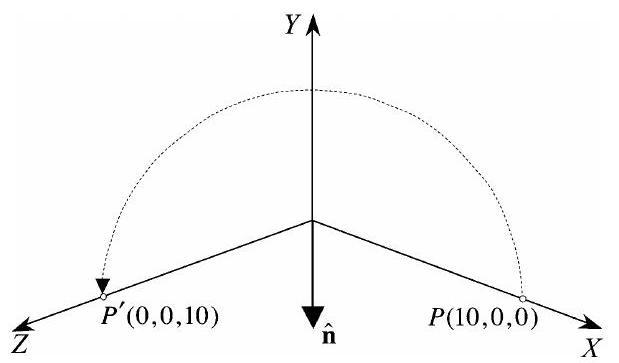
\includegraphics[max width=0.6\textwidth]{2023_01_16_a848224efad29cd66460g-097}
    \caption[short]{将点$P$从$180^{\circ}$旋转到$P^{\prime}$}
\end{figure}

接下来
$$
\mathbf{p}^{\prime}=\mathbf{p} \cos \alpha+\hat{\mathbf{n}}(\hat{\mathbf{n}} \cdot \mathbf{p}) K+(\hat{\mathbf{n}} \times \mathbf{p}) \sin \alpha
$$

且
$$
\begin{aligned}
\mathbf{p}^{\prime}= & \left(x_{p} \mathbf{i}+y_{p} \mathbf{j}+z_{p} \mathbf{k}\right) \cos \alpha+(a \mathbf{i}+b \mathbf{j}+c \mathbf{k})\left(a x_{p}+b y_{p}+c z_{p}\right) K \\
& +\left[\left(b z_{p}-c y_{p}\right) \mathbf{i}+\left(c x_{p}-a z_{p}\right) \mathbf{j}+\left(a y_{p}-b x_{p}\right) \mathbf{k}\right] \sin \alpha \\
\mathbf{p}^{\prime}= & {\left[x_{p} \cos \alpha+a\left(a x_{p}+b y_{p}+c z_{p}\right) K+\left(b z_{p}-c y_{p}\right) \sin \alpha\right] \mathbf{i} } \\
& +\left[y_{p} \cos \alpha+b\left(a x_{p}+b y_{p}+c z_{p}\right) K+\left(c x_{p}-a z_{p}\right) \sin \alpha\right] \mathbf{j} \\
& +\left[z_{p} \cos \alpha+c\left(a x_{p}+b y_{p}+c z_{p}\right) K+\left(a y_{p}-b x_{p}\right) \sin \alpha\right] \mathbf{k} \\
\mathbf{p}^{\prime}= & {\left[x_{p}\left(a^{2} K+\cos \alpha\right)+y_{p}(a b K-c \sin \alpha)+z_{p}(a c K+b \sin \alpha)\right] \mathbf{i} } \\
& +\left[x_{p}(a b K+c \sin \alpha)+y_{p}\left(b^{2} K+\cos \alpha\right)+z_{p}(b c K-a \sin \alpha)\right] \mathbf{j} \\
& +\left[x_{p}(a c K-b \sin \alpha)+y_{p}(b c K+a \sin \alpha)+z_{p}\left(c^{2} K+\cos \alpha\right)\right] \mathbf{k}
\end{aligned}
$$

它将解包到转换中:
$$
\left[\begin{array}{c}
x_{p}^{\prime} \\
y_{p}^{\prime} \\
z_{p}^{\prime}
\end{array}\right]=\left[\begin{array}{ccc}
a^{2} K+\cos \alpha & a b K-c \sin \alpha & a c K+b \sin \alpha \\
a b K+c \sin \alpha & b^{2} K+\cos \alpha & b c K-a \sin \alpha \\
a c K-b \sin \alpha & b c K+a \sin \alpha & c^{2} K+\cos \alpha
\end{array}\right]\left[\begin{array}{c}
x_{p} \\
y_{p} \\
z_{p}
\end{array}\right]
$$

其中
$$
K=1-\cos \alpha
$$

和用矩阵导出的变换是一样的。

让我们用一个容易验证的简单示例来测试转换。如果我们围绕$\hat{\mathbf{n}}=(1 / \sqrt{2}) \mathbf{i}+(1 / \sqrt{2}) \mathbf{k}$定义的轴旋转点$P(10,0,0), 180^{\circ}$,它应该被旋转到$P^{\prime}(0,0,10)$,如图6.9所示。因此,
$$
\begin{gathered}
\alpha=180^{\circ}, \quad \cos \alpha=-1, \quad \sin \alpha=0, \quad K=2, \\
a=\frac{1}{\sqrt{2}}, \quad b=0, \quad c=\frac{1}{\sqrt{2}}
\end{gathered}
$$

且
$$
\left[\begin{array}{c}
0 \\
0 \\
10
\end{array}\right]=\left[\begin{array}{ccc}
0 & 0 & 1 \\
0 & -1 & 0 \\
1 & 0 & 0
\end{array}\right]\left[\begin{array}{c}
10 \\
0 \\
0
\end{array}\right]
$$

这证实了我们的预测。

\section{总结}
在本章中,我们回顾了围绕三个笛卡尔轴之一旋转一个点的矩阵旋转变换。通过使用齐次坐标,可以将平移变换积分到围绕平行于一个笛卡尔轴的偏移轴旋转点。

复合旋转是通过组合表示围绕三个连续轴的单个旋转的矩阵来创建的。这样的旋转被称为欧拉旋转,有12种组合这些矩阵的方法。不幸的是,这种转换的问题之一是它们会受到万向节锁定的影响,在某些角度组合下会损失一个自由度。另一个问题是,虽然复合变换被广泛用于在世界空间中定位物体,但很难预测点在空间中如何移动。

最后,利用矩阵和向量建立了一个使一个点绕任意轴旋转的变换。

\subsection{变换总结}
\textbf{平移一个点}
$$
\mathbf{T}_{t_{x}, t_{y}, t_{z}}=\left[\begin{array}{cccc}
1 & 0 & 0 & t_{x} \\
0 & 1 & 0 & t_{y} \\
0 & 0 & 1 & t_{z} \\
0 & 0 & 0 & 1
\end{array}\right]
$$

\textbf{围绕$x-, y-, z$-轴旋转一个点}
$$
\begin{aligned}
\mathbf{R}_{\beta, x}= & {\left[\begin{array}{ccc}
1 & 0 & 0 \\
0 & \cos \beta & -\sin \beta \\
0 & \sin \beta & \cos \beta
\end{array}\right] } \\
\mathbf{R}_{\beta, y}= & {\left[\begin{array}{ccc}
\cos \beta & 0 & \sin \beta \\
0 & 1 & 0 \\
-\sin \beta & 0 & \cos \beta
\end{array}\right] } \\
\mathbf{R}_{\beta, z}= & {\left[\begin{array}{ccc}
\cos \beta & -\sin \beta & 0 \\
\sin \beta & \cos \beta & 0 \\
0 & 0 & 1
\end{array}\right] }
\end{aligned}
$$

\textbf{围绕偏移$x-, y-, z$-坐标轴旋转一个点}
$$
\begin{aligned}
\mathbf{R}_{\beta, x,\left(0, t_{y}, t_{z}\right)} & =\left[\begin{array}{cccc}
1 & 0 & 0 & 0 \\
0 & \cos \beta & -\sin \beta & t_{y}(1-\cos \beta)+t_{z} \sin \beta \\
0 & \sin \beta & \cos \beta & t_{z}(1-\cos \beta)-t_{y} \sin \beta \\
0 & 0 & 0 & 1
\end{array}\right] \\
\mathbf{R}_{\beta, y,\left(t_{x}, 0, t_{z}\right)} & =\left[\begin{array}{cccc}
\cos \beta & 0 & \sin \beta & t_{x}(1-\cos \beta)-t_{z} \sin \beta \\
0 & 1 & 0 & 0 \\
-\sin \beta & 0 & \cos \beta & t_{z}(1-\cos \beta)+t_{x} \sin \beta \\
0 & 0 & 0 & 1
\end{array}\right] \\
\mathbf{R}_{\beta, z,\left(t_{x}, t_{y}, 0\right)} & =\left[\begin{array}{cccc}
\cos \beta & -\sin \beta & 0 & t_{x}(1-\cos \beta)+t_{y} \sin \beta \\
\sin \beta & \cos \beta & 0 & t_{y}(1-\cos \beta)-t_{x} \sin \beta \\
0 & 0 & 1 & 0 \\
0 & 0 & 0 & 1
\end{array}\right]
\end{aligned}
$$

\textbf{绕任意轴旋转一点}
$$
\begin{aligned}
\mathbf{R}_{\alpha, \hat{\mathbf{n}}} & =\left[\begin{array}{ccc}
a^{2} K+\cos \alpha & a b K-c \sin \alpha & a c K+b \sin \alpha \\
a b K+c \sin \alpha & b^{2} K+\cos \alpha & b c K-a \sin \alpha \\
a c K-b \sin \alpha & b c K+a \sin \alpha & c^{2} K+\cos \alpha
\end{array}\right] \\
K & =1-\cos \alpha \\
\hat{\mathbf{n}} & =a \mathbf{i}+b \mathbf{j}+c \mathbf{k} .
\end{aligned}
$$

\section{样例}
下面是一些进一步使用上述思想的示例。在某些情况下,包括测试来确认结果。

\begin{example}
    建立一个旋转变换,使一个点围绕偏移于$y$-轴的轴旋转。
    
    设偏移轴与点$\left(t_{x}, 0, t_{z}\right)$相交。因此,这个旋转的齐次变换是
    $$
    \left[\begin{array}{c}
    x^{\prime} \\
    y^{\prime} \\
    z^{\prime} \\
    1
    \end{array}\right]=\mathbf{T}_{t_{x}, 0, t_{z}} \mathbf{R}_{\beta, y} \mathbf{T}_{-t_{x}, 0,-t_{z}}\left[\begin{array}{c}
    x \\
    y \\
    z \\
    1
    \end{array}\right]
    $$
    
    其中
    $$
    \begin{aligned}
    & \mathbf{T}_{-t_{x}, 0,-t_{z}} && \text { 创建临时原点 } \\
    & \mathbf{R}_{\beta, y} && \text { 围绕临时的 } y \text {轴旋转 }\beta \text{角度} \\
    & \mathbf{T}_{t_{x}, 0, t_{z}} && \text { 返回原来的坐标原点位置 }
    \end{aligned}
    $$
    
    且
    $$
    \begin{aligned}
    \mathbf{T}_{t_{x}, 0, t_{z}} & =\left[\begin{array}{llll}
    1 & 0 & 0 & t_{x} \\
    0 & 1 & 0 & 0 \\
    0 & 0 & 1 & t_{z} \\
    0 & 0 & 0 & 1
    \end{array}\right] \\
    \mathbf{T}_{-t_{x}, 0,-t_{z}} & =\left[\begin{array}{cccc}
    1 & 0 & 0 & -t_{x} \\
    0 & 1 & 0 & 0 \\
    0 & 0 & 1 & -t_{z} \\
    0 & 0 & 0 & 1
    \end{array}\right] \\
    \mathbf{R}_{\beta, y} & =\left[\begin{array}{cccc}
    \cos \beta & 0 & \sin \beta & 0 \\
    0 & 1 & 0 & 0 \\
    -\sin \beta & 0 & \cos \beta & 0 \\
    0 & 0 & 0 & 1
    \end{array}\right] .
    \end{aligned}
    $$
    
    因此,
    $$
    \begin{aligned}
    & \mathbf{T}_{t_{x}, 0, t_{z}} \mathbf{R}_{\beta, y} \mathbf{T}_{-t_{x}, 0,-t_{z}} \\
    &= {\left[\begin{array}{cccc}
    1 & 0 & 0 & t_{x} \\
    0 & 1 & 0 & 0 \\
    0 & 0 & 1 & t_{z} \\
    0 & 0 & 0 & 1
    \end{array}\right]\left[\begin{array}{cccc}
    \cos \beta & 0 & \sin \beta & 0 \\
    0 & 1 & 0 & 0 \\
    -\sin \beta & 0 & \cos \beta & 0 \\
    0 & 0 & 0 & 1
    \end{array}\right]\left[\begin{array}{cccc}
    1 & 0 & 0 & -t_{x} \\
    0 & 1 & 0 & 0 \\
    0 & 0 & 1 & -t_{z} \\
    0 & 0 & 0 & 1
    \end{array}\right] } \\
    &= {\left[\begin{array}{cccc}
    1 & 0 & 0 & t_{x} \\
    0 & 1 & 0 & 0 \\
    0 & 0 & 1 & t_{z} \\
    0 & 0 & 0 & 1
    \end{array}\right]\left[\begin{array}{cccc}
    \cos \beta & 0 & \sin \beta & -t_{x} \cos \beta-t_{z} \sin \beta \\
    0 & 1 & 0 & 0 \\
    -\sin \beta & 0 & \cos \beta & t_{x} \sin \beta-t_{z} \cos \beta \\
    0 & 0 & 0 & 1
    \end{array}\right] } \\
    &= {\left[\begin{array}{ccccc}
    \cos \beta & 0 & \sin \beta & t_{x}(1-\cos \beta)-t_{z} \sin \beta \\
    0 & 1 & 0 & 0 \\
    -\sin \beta & 0 & \cos \beta & t_{z}(1-\cos \beta)+t_{x} \sin \beta \\
    0 & 0 & 0 & 1
    \end{array}\right] }
    \end{aligned}
    $$
\end{example}

\begin{example}
    计算$\mathbf{R}_{\gamma, x} \mathbf{R}_{\beta, y} \mathbf{R}_{\alpha, x}$的旋转变换,看看当$\alpha=\beta=\gamma=90^{\circ}$时,它是否会出现万向锁。旋转轴和角度是多少?
    
    使用符号$c_{\beta}=\cos \beta$和$s_{\beta}=\sin \beta$,复合转换为
    $$
    \begin{aligned}
    \mathbf{R}_{\gamma, x} \mathbf{R}_{\beta, y} \mathbf{R}_{\alpha, x} & =\left[\begin{array}{ccc}
    1 & 0 & 0 \\
    0 & c_{\gamma} & -s_{\gamma} \\
    0 & s_{\gamma} & c_{\gamma}
    \end{array}\right]\left[\begin{array}{ccc}
    c_{\beta} & 0 & s_{\beta} \\
    0 & 1 & 0 \\
    -s_{\beta} & 0 & c_{\beta}
    \end{array}\right]\left[\begin{array}{ccc}
    1 & 0 & 0 \\
    0 & c_{\alpha} & -s_{\alpha} \\
    0 & s_{\alpha} & c_{\alpha}
    \end{array}\right] \\
    & =\left[\begin{array}{ccc}
    c_{\beta} & s_{\beta} s_{\alpha} & s_{\beta} c_{\alpha} \\
    s_{\gamma} s_{\beta} & \left(c_{\gamma} c_{\alpha}-s_{\gamma} c_{\beta} s_{\alpha}\right) & \left(-c_{\gamma} s_{\alpha}-s_{\gamma} c_{\beta} c_{\alpha}\right) \\
    -c_{\gamma} s_{\beta} & \left(s_{\gamma} c_{\alpha}+c_{\gamma} c_{\beta} s_{\alpha}\right) & \left(-s_{\gamma} s_{\alpha}+c_{\gamma} c_{\beta} c_{\alpha}\right)
    \end{array}\right] \\
    \mathbf{R}_{90^{\circ}, x} \mathbf{R}_{90^{\circ}, y} \mathbf{R}_{90^{\circ}, x} & =\left[\begin{array}{ccc}
    0 & 1 & 0 \\
    1 & 0 & 0 \\
    0 & 0 & -1
    \end{array}\right] .
    \end{aligned}
    $$
    
    图$6.10$显示了立方体在旋转的每个阶段,很明显,万向节锁不存在,因为立方体通过其每个正交轴旋转。旋转轴是通过顶点0和6,即$\left[\begin{array}{lll}1 & 1 & 0\end{array}\right]^{\mathrm{T}}$,旋转角度为$180^{\circ}$。
    
    \begin{figure}[h!]
        \centering
        \subfigure[caption]{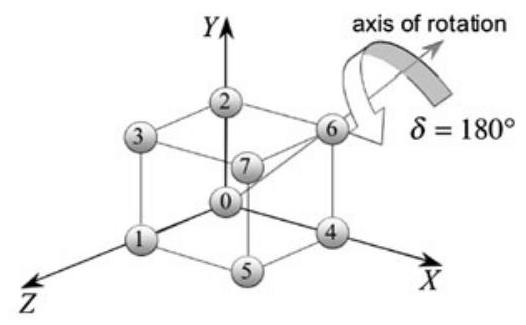
\includegraphics[max width=0.35\textwidth]{2023_01_16_a848224efad29cd66460g-101}}
        \subfigure[caption]{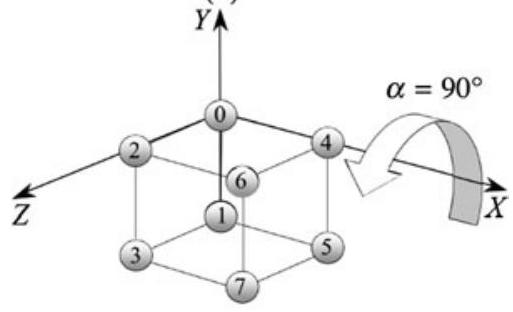
\includegraphics[max width=0.35\textwidth]{2023_01_16_a848224efad29cd66460g-101(2)}}\\
        \subfigure[caption]{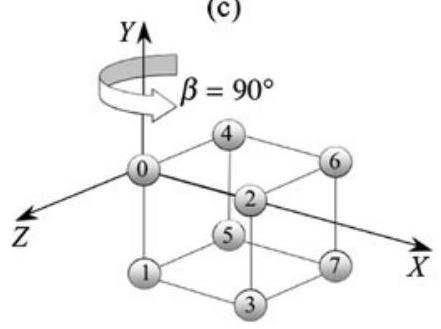
\includegraphics[max width=0.35\textwidth]{2023_01_16_a848224efad29cd66460g-101(1)}}
        \subfigure[caption]{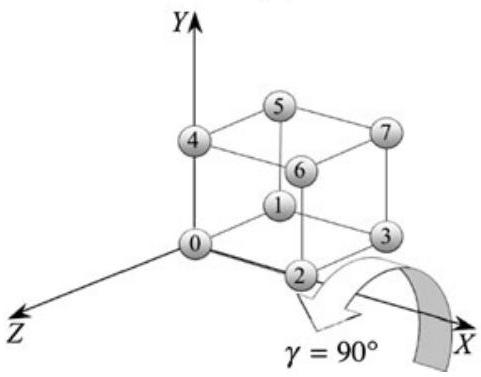
\includegraphics[max width=0.35\textwidth]{2023_01_16_a848224efad29cd66460g-101(3)}}
        \caption[short]{单元立方体在三次旋转之前和过程中的四个视图$\mathbf{R}_{90^{\circ}, x} \mathbf{R}_{90^{\circ}, y} \mathbf{R}_{90^{\circ}, x}$}
    \end{figure}
\end{example}

\begin{example}
    证明任意轴上旋转点的旋转矩阵适用于三个笛卡尔轴。
    
    从这个矩阵开始:
    
    $$
    \begin{aligned}
    \mathbf{R}_{\alpha, \hat{\mathbf{n}}} & =\left[\begin{array}{ccc}
    a^{2} K+\cos \alpha & a b K-c \sin \alpha & a c K+b \sin \alpha \\
    a b K+c \sin \alpha & b^{2} K+\cos \alpha & b c K-a \sin \alpha \\
    a c K-b \sin \alpha & b c K+a \sin \alpha & c^{2} K+\cos \alpha
    \end{array}\right] \\
    K & =1-\cos \alpha \\
    \hat{\mathbf{n}} & =a \mathbf{i}+b \mathbf{j}+c \mathbf{k} .
    \end{aligned}
    $$
    
    绕$x$轴旋转:
    $$
    \hat{\mathbf{n}}=a \mathbf{i}
    $$
    
    因此,$a=1$, $b=c=0$:
    $$
    \mathbf{R}_{\alpha, x}=\left[\begin{array}{ccc}
    1 & 0 & 0 \\
    0 & \cos \alpha & -\sin \alpha \\
    0 & \sin \alpha & \cos \alpha
    \end{array}\right] .
    $$
    
    绕$y$轴旋转:
    $$
    \hat{\mathbf{n}}=b \mathbf{j}
    $$
    
    因此, $b=1$, $a=c=0$ :
    $$
    \mathbf{R}_{\alpha, y}=\left[\begin{array}{ccc}
    \cos \alpha & 0 & \sin \alpha \\
    0 & 1 & 0 \\
    -\sin \alpha & 0 & \cos \alpha
    \end{array}\right]
    $$
    
    绕$z$轴旋转:
    $$
    \hat{\mathbf{n}}=c \mathbf{k}
    $$
    
    因此,$c=1$,$a=b=0$ :
    
    $$
    \mathbf{R}_{\alpha, z}=\left[\begin{array}{ccc}
    \cos \alpha & -\sin \alpha & 0 \\
    \sin \alpha & \cos \alpha & 0 \\
    0 & 0 & 1
    \end{array}\right]
    $$
    
    这是正确的。
\end{example}

\begin{example}
    计算旋转变换,使一个点围绕一个与$\left[\begin{array}{lll}1 & 1 & 1\end{array}\right]^{\mathrm {T}}$对齐的轴旋转$180^{\circ}$。举个例子,通过这个变换将一个点旋转两次将其返回到它原来的位置。
    
    从矩阵开始:
    $$
    \begin{aligned}
    \mathbf{R}_{\alpha, \hat{\mathbf{n}}} & =\left[\begin{array}{ccc}
    a^{2} K+\cos \alpha & a b K-c \sin \alpha & a c K+b \sin \alpha \\
    a b K+c \sin \alpha & b^{2} K+\cos \alpha & b c K-a \sin \alpha \\
    a c K-b \sin \alpha & b c K+a \sin \alpha & c^{2} K+\cos \alpha
    \end{array}\right] \\
    K & =1-\cos \alpha \\
    \hat{\mathbf{n}} & =a \mathbf{i}+b \mathbf{j}+c \mathbf{k} .
    \end{aligned}
    $$
    
    因此,给出 $\mathbf{n}=\mathbf{i}+\mathbf{j}+\mathbf{k}$
    
    $$
    \hat{\mathbf{n}}=\frac{1}{\sqrt{3}} \mathbf{i}+\frac{1}{\sqrt{3}} \mathbf{j}+\frac{1}{\sqrt{3}} \mathbf{k}
    $$
    
    且
    
    $$
    a=b=c=\frac{1}{\sqrt{3}} \text {. }
    $$
    
    给出 $\alpha=180^{\circ}, \cos \alpha=-1, \sin \alpha=0$ 且 $K=2$, 矩阵就变成了:
    $$
    \mathbf{R}_{180^{\circ}, \hat{\mathbf{n}}}=\left[\begin{array}{ccc}
    -1 / 3 & 2 / 3 & 2 / 3 \\
    2 / 3 & -1 / 3 & 2 / 3 \\
    2 / 3 & 2 / 3 & -1 / 3
    \end{array}\right] \text {. }
    $$
    
    这个矩阵与自身相乘必然得到单位矩阵:
    $$
    \begin{aligned}
    \mathbf{R}_{180^{\circ}, \hat{\mathbf{n}}} \mathbf{R}_{180^{\circ}, \hat{\mathbf{n}}} & =\left[\begin{array}{ccc}
    -1 / 3 & 2 / 3 & 2 / 3 \\
    2 / 3 & -1 / 3 & 2 / 3 \\
    2 / 3 & 2 / 3 & -1 / 3
    \end{array}\right]\left[\begin{array}{ccc}
    -1 / 3 & 2 / 3 & 2 / 3 \\
    2 / 3 & -1 / 3 & 2 / 3 \\
    2 / 3 & 2 / 3 & -1 / 3
    \end{array}\right] \\
    & =\left[\begin{array}{ccc}
    1 & 0 & 0 \\
    0 & 1 & 0 \\
    0 & 0 & 1
    \end{array}\right]
    \end{aligned}
    $$
    
    这证实了任意点经过这个旋转矩阵旋转两次后都回到了原点。
\end{example}

\chap{空间中的四元数}
\section{介绍}
在本章中,我们将展示如何使用四元数来围绕任意轴旋转向量。我们首先回顾了一些与四元数相关的历史,特别是本杰明·奥林德·罗德里格斯(Benjamin Olinde Rodrigues)的作用,他发现了旋转变换中半角的重要性。

对于特定的四元数积,当四元数表示为
$$
q=[\cos \theta, \sin \theta \mathbf{v}]
$$

一个向量围绕轴$\mathbf{v}$旋转一个角度$\theta$。但是,我们会发现,对于三重四元数的乘积,当四元数表示为
$$
q=\left[\cos \frac{1}{2} \theta, \sin \frac{1}{2} \theta \mathbf{v}\right]
$$

一个向量围绕轴$\mathbf{v}$旋转一个角度$\theta$。这种半角表示是罗德里格斯发现的。

关于组合代数的简短部分揭示了四元数是相当特殊的,并告诉我们为什么 Hamilton 不能识别基于超复数$z=s+ i+ bj $的代数。

然后,我们检查了各种四元数乘积,以发现它们的旋转性质。这从两个正交四元数开始,然后转向使用三重$q p q^{-1}$的一般情况,其中$q$是一个单位范数四元数,$p$是一个纯四元数。

本章介绍了两种将四元数乘积表示为矩阵的方法,这两种方法依次编码特征向量和特征值。最后,我们研究如何插值四元数。

我们继续将四元数表示为有序对,用斜体小写字母表示四元数,用粗体小写字母表示向量。

\section{一点历史}
本杰明·罗德里格斯(Benjamin Olinde Rodrigues, 1795-1851)出生于法国波尔多。他在巴黎学习,并于1816年获得博士学位,时年21岁。他论文的主题是求解 Legendre 多项式, Rodrigues 提出了一个解,这个解至今仍被称为 Rodrigues 公式。

虽然他从事政治和银行业,但他的博士研究证实他不仅仅是一个“娱乐”数学家,因为在1840年,他在《纯数学年鉴》(Annales de Mathématiques Pures et Appliquées)上发表了一篇关于变换群[20]的数学论文。该文包含了一个公式,其描述了一个几何结构,即两个连续的围绕不同的轴的旋转,等价于第三个围绕另一个轴的旋转。今天,我们知道这种对应称为Euler-Rodrigues参数化。欧拉在1775年已经证明了一次旋转可以表示围绕不同轴的两次连续旋转,但没有提供代数解。

如果我们将一个关于轴向量$\mathbf{a}$的旋转$\alpha$表示为$\mathbf{R}_{\alpha, \mathbf{a}}$,那么Rodrigues提供了一个解决方案
$$
\mathbf{R}_{\gamma, \mathbf{n}}=\mathbf{R}_{\alpha, \mathbf{l}} \mathbf{R}_{\beta, \mathbf{m}}
$$

形式为
\begin{align}
& \cos \frac{1}{2} \gamma=\cos \frac{1}{2} \alpha \cos \frac{1}{2} \beta-\sin \frac{1}{2} \alpha \sin \frac{1}{2} \beta \mathbf{l} \cdot \mathbf{m} \\
& \sin \frac{1}{2} \gamma \mathbf{n}=\sin \frac{1}{2} \alpha \cos \frac{1}{2} \beta \mathbf{l}+\cos \frac{1}{2} \alpha \sin \frac{1}{2} \beta \mathbf{m}+\sin \frac{1}{2} \alpha \sin \frac{1}{2} \beta \mathbf{l} \times \mathbf{m} .
\end{align}

Rodrigues没有使用(7.1)和(7.2)中使用的向量符号,因为这还没有被Hamilton定义,但他确实使用了这些向量积的代数等价物。图$7.1$显示了罗德里格斯使用的由轴和旋转角组成的球形三角形。

\begin{figure}[h!]
    \centering
    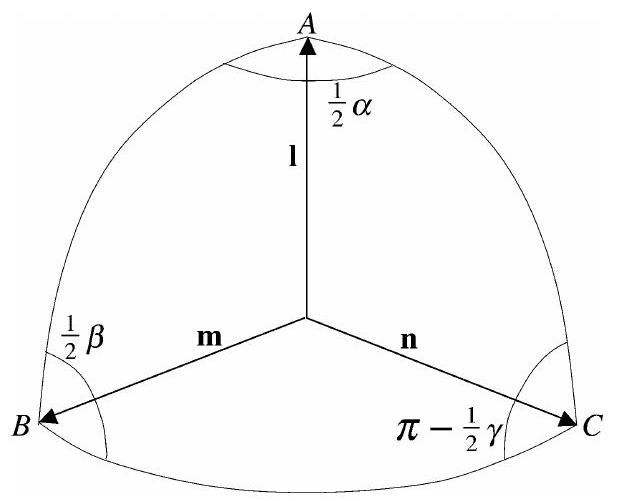
\includegraphics[max width=0.5\textwidth]{2023_01_16_a848224efad29cd66460g-105}
    \caption[short]{显示$\mathbf{l}$、$\mathbf{m}$和$\mathbf{n}$的Rodrigues球面三角形}
\end{figure}

式(7.1)和式(7.2)包含了一些四元数乘积所熟悉的特征,这些特征在下面的分析中变得很明显。我们从定义四元数开始

$$
\begin{aligned}
q_{l} & =\left[\cos \frac{1}{2} \alpha, \sin \frac{1}{2} \alpha \mathbf{l}\right] \\
q_{m} & =\left[\cos \frac{1}{2} \beta, \sin \frac{1}{2} \beta \mathbf{m}\right] \\
q_{n} & =\left[\cos \frac{1}{2} \gamma, \sin \frac{1}{2} \gamma \mathbf{n}\right]
\end{aligned}
$$

且乘积形式为
\begin{align}
q_{n}  =& q_{l} q_{m} \notag\\
=& \left[\cos \frac{1}{2} \alpha, \sin \frac{1}{2} \alpha \mathbf{l}\right]\left[\cos \frac{1}{2} \beta, \sin \frac{1}{2} \beta \mathbf{m}\right] \notag\\
=& \left[\cos \frac{1}{2} \alpha \cos \frac{1}{2} \beta-\sin \frac{1}{2} \alpha \sin \frac{1}{2} \beta \mathbf{l} \cdot \mathbf{m},\right. \notag\\
& \left.\sin \frac{1}{2} \alpha \cos \frac{1}{2} \beta \mathbf{l}+\cos \frac{1}{2} \alpha \sin \frac{1}{2} \beta \mathbf{m}+\sin \frac{1}{2} \alpha \sin \frac{1}{2} \beta \mathbf{l} \times \mathbf{m}\right] \notag\\
\cos \frac{1}{2} \gamma = & \cos \frac{1}{2} \alpha \cos \frac{1}{2} \beta-\sin \frac{1}{2} \alpha \sin \frac{1}{2} \beta \mathbf{l} \cdot \mathbf{m} \\
\sin \frac{1}{2} \gamma \mathbf{n} =& \sin \frac{1}{2} \alpha \cos \frac{1}{2} \beta \mathbf{l}+\cos \frac{1}{2} \alpha \sin \frac{1}{2} \beta \mathbf{m}+\sin \frac{1}{2} \alpha \sin \frac{1}{2} \beta \mathbf{l} \times \mathbf{m}
\end{align}

其中(7.3)和(7.4)分别与(7.1)和(7.2)相同。虽然Rodrigues没有发明四元数的形式
$$
q=s+a i+b j+c k,
$$

他在 Hamilton 之前就发现了四元数积的系数。这就是生活!\footnote{译注,法语:C'est la vie!}

Hamilton 在1843年10月发明了四元数,同年12月,他的朋友、爱尔兰数学家约翰·托马斯·格雷夫斯(John Thomas Graves, 1806-1870)发明了八度音阶,最终被称为八元数。英国数学家亚瑟·凯利(Arthur Cayley, 1821-1895)也对 Hamilton 的四元数很感兴趣,并于1845年独立发明了八元数。八元数最终被称为Cayley数而不是八元数,只是因为Graves直到1848年才发表了他的结果——比Cayley晚了3年!

正如四元数可以用复数的有序对来定义一样,八度或八元数也可以用四元数的有序对来定义。

\subsection{组合代数}
当一个特定的定律构成一个代数的基础时,它被称为组合代数。例如,我们知道在普通算术中
$$
a^{2} b^{2}=(a b)^{2} \qquad a, b \in \mathbb{R}
$$
比如
$$
3^{2} 4^{2}=12^{2}
$$
其中平方定律就是组合定律。

我们在第四章中发现,对于两个复数:
$$
\begin{aligned}
\left|z_{1}\right|\left|z_{2}\right| & =\left|z_{1} z_{2}\right| \qquad z_{1}, z_{2} \in \mathbb{C} \\
\left|z_{1}\right|^{2}\left|z_{2}\right|^{2} & =\left|z_{1} z_{2}\right|^{2} .
\end{aligned}
$$
举个例子, 给出
$$
\begin{aligned}
& z_{1}=a_{1}+b_{1} i \\
& z_{2}=a_{2}+b_{2} i
\end{aligned}
$$
然后
$$
\left(a_{1}^{2}+b_{1}^{2}\right)\left(a_{2}^{2}+b_{2}^{2}\right)=\left(a_{1} a_{2}-b_{1} b_{2}\right)^{2}+\left(a_{1} b_{2}+a_{2} b_{1}\right)^{2}
$$
这是一个2平方定律。

在第5章中,我们注意到对于两个四元数:
$$
\left|q_{a}\right|^{2}\left|q_{b}\right|^{2}=\left|q_{a} q_{b}\right|^{2} \quad q_{a}, q_{b} \in \mathbb{H} .
$$
举个例子, 给出
$$
\begin{aligned}
q_{a} & =\left[s_{a}, x_{a} \mathbf{i}+y_{a} \mathbf{j}+z_{a} \mathbf{k}\right] \\
q_{b} & =\left[s_{b}, x_{b} \mathbf{i}+y_{b} \mathbf{j}+z_{b} \mathbf{k}\right]
\end{aligned}
$$
然后
$$
\begin{aligned}
\left(s_{a}^{2}+x_{a}^{2}+y_{a}^{2}+z_{a}^{2}\right)\left(s_{b}^{2}+x_{b}^{2}+y_{b}^{2}+z_{b}^{2}\right)= & \left(s_{a} s_{b}-x_{a} x_{b}-y_{a} y_{b}-z_{a} z_{b}\right)^{2} \\
& +\left(s_{a} x_{b}+s_{b} x_{a}+y_{a} z_{b}-y_{b} z_{a}\right)^{2} \\
& +\left(s_{a} y_{b}+s_{b} y_{a}+z_{a} x_{b}-z_{b} x_{a}\right)^{2} \\
& +\left(s_{a} z_{b}+s_{b} z_{a}+x_{a} y_{b}-x_{b} y_{a}\right)^{2}
\end{aligned}
$$
这是四方定律。

除了复数,四元数在数学系统中占据着中心位置,今天有四个这样的组合代数:实$\mathbb{R}$、复$\mathbb{C}$、四元数$\mathbb{H}$和八元数$\mathbb{O}$,它们遵循$n$-平方的恒等式来计算它们的规范。1898年,德国数学家阿道夫·赫维茨(Adolf Hurwitz, 1859-1919)证明,只有当$n$等于1、2、4和8时,$n$的平方和与$n$的平方和的乘积才等于$n$的平方和,其中$n$用实数、复数、四元数和八元数表示。这就是所谓的“赫维茨定理”或“1,2,4,8定理”。没有其他系统是可能的,这表明四元数在数学领域是多么重要。因此,Hamilton对三元体系的探索是徒劳的,因为不存在三平方恒等式。

现在让我们研究如何使用四元数来围绕任意轴旋转向量。

\section{四元数乘积}
四元数$q$是标量$s$和向量$\mathbf{v}$的并集:
$$
q=[s, \mathbf{v}] \quad s \in \mathbb{R}, \mathbf{v} \in \mathbb{R}^{3}
$$

如果我们用$\mathbf{v}$的分量来表示它,我们有
$$
q=[s, x \mathbf{i}+y \mathbf{j}+z \mathbf{k}] \quad s, x, y, z \in \mathbb{R} .
$$

Hamilton曾希望四元数可以像复数转子一样使用,后者我们在第二章中看到了
$$
\mathbf{R}_{\theta}=\cos \theta+i \sin \theta
$$

将一个复数旋转$\theta$。单位范数四元数$q$可以用来旋转存储为纯四元数$p$的向量吗?是的,但只是在有限的意义上。为了理解这一点,让我们构造一个单位范数四元数$q$和一个纯四元数$p$的乘积。单位范数四元数$q$定义为
\begin{align}
\begin{aligned}
q & =[s, \lambda \hat{\mathbf{v}}] \quad s, \lambda \in \mathbb{R}, \hat{\mathbf{v}} \in \mathbb{R}^{3} \\
|\hat{\mathbf{v}}| & =1 \\
s^{2}+\lambda^{2} & =1
\end{aligned}
\end{align}
纯四元数$p$存储要旋转的向量$\mathbf{p}$:
$$
p=[0, \mathbf{p}] \quad \mathbf{p} \in \mathbb{R}^{3} .
$$

让我们计算乘积$p^{\prime}=q p$,并检查$p^{\prime}$的向量部分,看看$ \mathbf{p}$是否被旋转:
\begin{align}
\begin{aligned}
p^{\prime} & =q p \\
& =[s, \lambda \hat{\mathbf{v}}][0, \mathbf{p}] \\
& =[-\lambda \hat{\mathbf{v}} \cdot \mathbf{p}, s \mathbf{p}+\lambda \hat{\mathbf{v}} \times \mathbf{p}] .
\end{aligned}
\end{align}

我们可以从(7.6)中看到,结果是一个具有标量和向量分量的一般四元数。

\subsection{特殊情况}
上面提到的“狭义”是$\hat{\mathbf{v}}$必须垂直于$\mathbf{p}$,这使得点积项$-\lambda \hat{\mathbf{v}} \cdot \mathbf{p}$在(7.6)中消失,我们只剩下纯四元数

The 'restricted sense' referred to above is that $\hat{\mathbf{v}}$ must be perpendicular to $\mathbf{p}$, which makes the dot product term $-\lambda \hat{\mathbf{v}} \cdot \mathbf{p}$ in (7.6) vanish, and we are left with the pure quaternion

$$
p^{\prime}=[0, s \mathbf{p}+\lambda \hat{\mathbf{v}} \times \mathbf{p}] .
$$

Figure $7.2$ illustrates this scenario, where $\mathbf{p}$ is perpendicular to $\hat{\mathbf{v}}$, and $\hat{\mathbf{v}} \times \mathbf{p}$ is perpendicular to the plane containing $\mathbf{p}$ and $\hat{\mathbf{v}}$. Now because $\hat{\mathbf{v}}$ is a unit vector, $|\mathbf{p}|=|\hat{\mathbf{v}} \times \mathbf{p}|$, which means that we have two orthogonal vectors, i.e. $\mathbf{p}$ and $\hat{\mathbf{v}} \times \mathbf{p}$, with the same length. Therefore, to rotate $\mathbf{p}$ about $\hat{\mathbf{v}}$, all that we have to do is make $s=\cos \theta$ and $\lambda=\sin \theta$ in (7.7):

Fig. 7.2 Three orthogonal vectors $\mathbf{p}, \hat{\mathbf{v}}$ and $\hat{\mathbf{v}} \times \mathbf{p}$

Fig. 7.3 The vector $2 \mathbf{i}$ is rotated $45^{\circ}$ by the quaternion $q=\left[\frac{\sqrt{2}}{2}, \frac{\sqrt{2}}{2} \mathbf{k}\right]$
\begin{figure}
    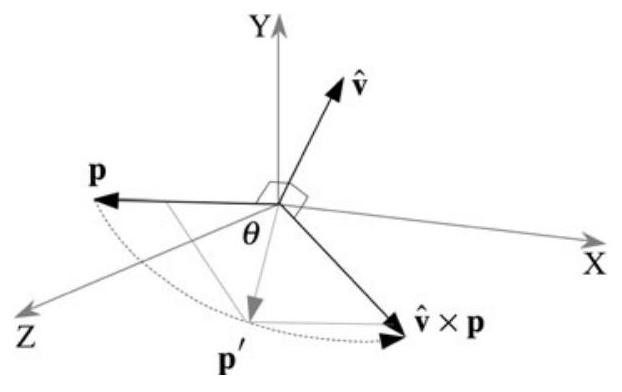
\includegraphics[max width=0.5\textwidth, center]{2023_01_16_a848224efad29cd66460g-109}
    \caption[short]{title}
\end{figure}




$$
\begin{aligned}
p^{\prime} & =\left[0, \mathbf{p}^{\prime}\right] \\
& =[0, \cos \theta \mathbf{p}+\sin \theta \hat{\mathbf{v}} \times \mathbf{p}]
\end{aligned}
$$

For example, to rotate a vector about the $z$-axis, $q$ 's vector $\hat{\mathbf{v}}$ must be aligned with the $z$-axis as shown in Fig. 7.3. If we make the angle of rotation $\theta=45^{\circ}$ then

$$
\begin{aligned}
q & =[s, \lambda \hat{\mathbf{v}}] \\
& =[\cos \theta, \sin \theta \mathbf{k}] \\
& =\left[\frac{\sqrt{2}}{2}, \frac{\sqrt{2}}{2} \mathbf{k}\right]
\end{aligned}
$$

and if the vector to be rotated is $\mathbf{p}=2 \mathbf{i}$, then

$$
\begin{aligned}
p & =[0, \mathbf{p}] \\
& =[0,2 \mathbf{i}] .
\end{aligned}
$$

There are now four product combinations worth exploring: $q p, p q, q^{-1} p$ and $p q^{-1}$. It's not worth considering $q p^{-1}$ and $p^{-1} q$ as $p^{-1}$ simply reverses the direction of $\mathbf{p}$. Let's start with $q p$ :

$$
\begin{aligned}
p^{\prime} & =q p \\
& =\left[\frac{\sqrt{2}}{2}, \frac{\sqrt{2}}{2} \mathbf{k}\right][0,2 \mathbf{i}] \\
& =\left[0,2 \frac{\sqrt{2}}{2} \mathbf{i}+2 \frac{\sqrt{2}}{2} \mathbf{k} \times \mathbf{i}\right] \\
& =[0, \sqrt{2} \mathbf{i}+\sqrt{2} \mathbf{j}]
\end{aligned}
$$

and $\mathbf{p}$ has been rotated $45^{\circ}$ to $\mathbf{p}^{\prime}=\sqrt{2} \mathbf{i}+\sqrt{2} \mathbf{j}$.

Next, $p q$ :

$$
\begin{aligned}
p^{\prime} & =p q \\
& =[0,2 \mathbf{i}]\left[\frac{\sqrt{2}}{2}, \frac{\sqrt{2}}{2} \mathbf{k}\right] \\
& =\left[0,2 \frac{\sqrt{2}}{2} \mathbf{i}-2 \frac{\sqrt{2}}{2} \mathbf{k} \times \mathbf{i}\right] \\
& =[0, \sqrt{2} \mathbf{i}-\sqrt{2} \mathbf{j}]
\end{aligned}
$$

and $\mathbf{p}$ has been rotated $-45^{\circ}$ to $\mathbf{p}^{\prime}=\sqrt{2} \mathbf{i}-\sqrt{2} \mathbf{j}$.

Next, $q^{-1} p$, and as $q$ is a unit-norm quaternion, $q^{-1}=q^{*}$ :

$$
\begin{aligned}
p^{\prime} & =q^{-1} p \\
& =\left[\frac{\sqrt{2}}{2},-\frac{\sqrt{2}}{2} \mathbf{k}\right][0,2 \mathbf{i}] \\
& =\left[0,2 \frac{\sqrt{2}}{2} \mathbf{i}-2 \frac{\sqrt{2}}{2} \mathbf{k} \times \mathbf{i}\right] \\
& =[0, \sqrt{2} \mathbf{i}-\sqrt{2} \mathbf{j}]
\end{aligned}
$$

and $\mathbf{p}$ has been rotated $-45^{\circ}$ to $\mathbf{p}^{\prime}=\sqrt{2} \mathbf{i}-\sqrt{2} \mathbf{j}$.

Finally, $p q^{-1}$ :

$$
\begin{aligned}
p^{\prime} & =p q^{-1} \\
& =[0,2 \mathbf{i}]\left[\frac{\sqrt{2}}{2},-\frac{\sqrt{2}}{2} \mathbf{k}\right] \\
& =\left[0,2 \frac{\sqrt{2}}{2} \mathbf{i}+2 \frac{\sqrt{2}}{2} \mathbf{k} \times \mathbf{i}\right] \\
& =[0, \sqrt{2} \mathbf{i}+\sqrt{2} \mathbf{j}]
\end{aligned}
$$

and $\mathbf{p}$ has been rotated $45^{\circ}$ to $\mathbf{p}^{\prime}=\sqrt{2} \mathbf{i}+\sqrt{2} \mathbf{j}$. Thus, for orthogonal quaternions, $\theta$ is the angle of rotation, then

$$
\begin{aligned}
& q p=p q^{-1} \\
& p q=q^{-1} p
\end{aligned}
$$

Fig. 7.4 Rotating the vector $\mathbf{p}=2 \mathbf{i}$ by the quaternion $q=[\cos \theta, \sin \theta \hat{\mathbf{v}}]$

\begin{center}
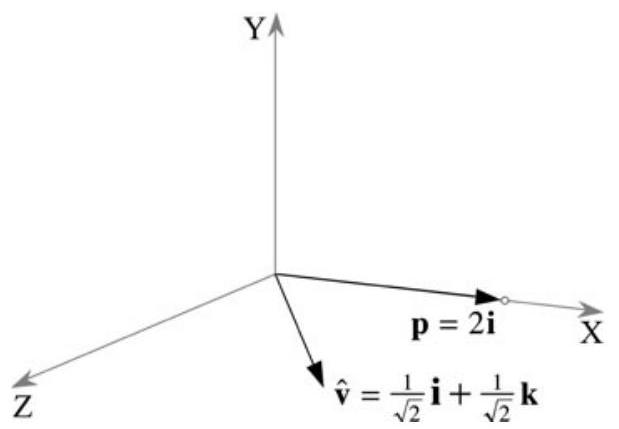
\includegraphics[max width=\textwidth]{2023_01_16_a848224efad29cd66460g-111}
\end{center}

Before moving on, let's see what happens to the product $q p$ when $\theta=180^{\circ}$ :

$$
\begin{aligned}
p^{\prime} & =q p \\
& =[-1, \mathbf{0}][0,2 \mathbf{i}] \\
& =[0,-2 \mathbf{i}]
\end{aligned}
$$

and $\mathbf{p}$ has been rotated $180^{\circ}$ to $\mathbf{p}^{\prime}=-2 \mathbf{i}$.

Note that in all the above products, the vector has not been scaled during the rotation. This is because $q$ is a unit-norm quaternion. Now let's see what happens if we change the angle between $\hat{\mathbf{v}}$ and $\mathbf{p}$. Let's reduce the angle to $45^{\circ}$ and retain $q$ 's unit vector, as shown in Fig. 7.4. Therefore,

$$
\begin{aligned}
\hat{\mathbf{v}} & =\frac{1}{\sqrt{2}} \mathbf{i}+\frac{1}{\sqrt{2}} \mathbf{k} \\
q & =[\cos \theta, \sin \theta \hat{\mathbf{v}}] \\
p & =[0, \mathbf{p}] .
\end{aligned}
$$

This time we must include the dot product term $-\sin \theta \hat{\mathbf{v}} \cdot \mathbf{p}$, as it is no longer zero:

$$
\begin{aligned}
p^{\prime} & =q p \\
& =[\cos \theta, \sin \theta \hat{\mathbf{v}}][0, \mathbf{p}] \\
& =[-\sin \theta \hat{\mathbf{v}} \cdot \mathbf{p}, \cos \theta \mathbf{p}+\sin \theta \hat{\mathbf{v}} \times \mathbf{p}] .
\end{aligned}
$$

Substituting $\hat{\mathbf{v}}, \mathbf{p}$ and $\theta=45^{\circ}$ in $(7.8)$, we have

$$
\begin{aligned}
p^{\prime} & =\left[-\frac{\sqrt{2}}{2}\left(\frac{1}{\sqrt{2}} \mathbf{i}+\frac{1}{\sqrt{2}} \mathbf{k}\right) \cdot(2 \mathbf{i}), \frac{\sqrt{2}}{2} 2 \mathbf{i}+\frac{\sqrt{2}}{2}\left(\frac{1}{\sqrt{2}} \mathbf{i}+\frac{1}{\sqrt{2}} \mathbf{k}\right) \times 2 \mathbf{i}\right] \\
& =[-1, \sqrt{2} \mathbf{i}+\mathbf{j}]
\end{aligned}
$$

which, unfortunately, is no longer a pure quaternion. It has not been rotated $45^{\circ}$, and the vector's norm is reduced to $\sqrt{3}$ ! Multiplying the vector by a non-orthogonal quaternion has converted some of the vector information into the quaternion's scalar component. Fig. 7.5 The vector $2 \mathbf{i}$ is rotated $90^{\circ}$ to $\mathbf{i}+\sqrt{2} \mathbf{j}+\mathbf{k}$

\begin{center}
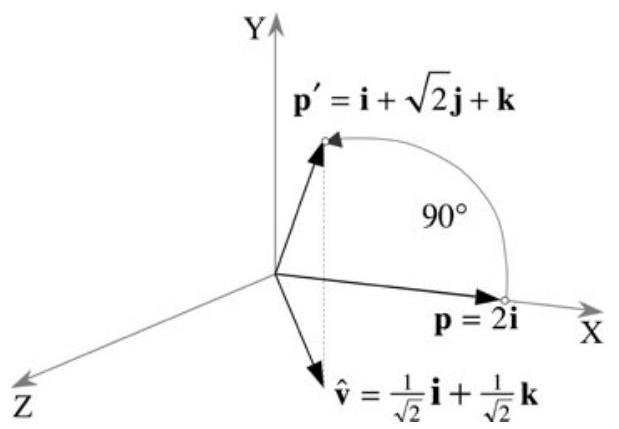
\includegraphics[max width=\textwidth]{2023_01_16_a848224efad29cd66460g-112}
\end{center}

\subsection{一般情况}
Not to worry. Could it be that an inverse quaternion reverses the operation? Let's see what happens if we post-multiply $q p$ by $q^{-1}$.

Given

$$
q=\left[\cos \theta, \sin \theta\left(\frac{1}{\sqrt{2}} \mathbf{i}+\frac{1}{\sqrt{2}} \mathbf{k}\right)\right]
$$

then

$$
\begin{aligned}
q^{-1} & =\left[\cos \theta,-\sin \theta\left(\frac{1}{\sqrt{2}} \mathbf{i}+\frac{1}{\sqrt{2}} \mathbf{k}\right)\right] \\
& =\left[\frac{\sqrt{2}}{2}, \frac{\sqrt{2}}{2}\left(\frac{1}{\sqrt{2}} \mathbf{i}+\frac{1}{\sqrt{2}} \mathbf{k}\right)\right] \\
& =\frac{1}{2}[\sqrt{2},-\mathbf{i}-\mathbf{k}] .
\end{aligned}
$$

Therefore, post-multiplying (7.9) by $q^{-1}$ we have

$$
\begin{aligned}
q p q^{-1} & =[-1, \sqrt{2} \mathbf{i}+\mathbf{j}] \frac{1}{2}[\sqrt{2},-\mathbf{i}-\mathbf{k}] \\
& =\frac{1}{2}[-\sqrt{2}-(\sqrt{2} \mathbf{i}+\mathbf{j}) \cdot(-\mathbf{i}-\mathbf{k}), \mathbf{i}+\mathbf{k}+\sqrt{2}(\sqrt{2} \mathbf{i}+\mathbf{j})-\mathbf{i}+\sqrt{2} \mathbf{j}+\mathbf{k}] \\
& =\frac{1}{2}[-\sqrt{2}+\sqrt{2}, \mathbf{i}+\mathbf{k}+2 \mathbf{i}+\sqrt{2} \mathbf{j}-\mathbf{i}+\sqrt{2} \mathbf{j}+\mathbf{k}] \\
& =[0, \mathbf{i}+\sqrt{2} \mathbf{j}+\mathbf{k}]
\end{aligned}
$$

which is a pure quaternion. Furthermore, there's no scaling as its norm is still 2, but the vector has been rotated $90^{\circ}$ rather than $45^{\circ}$, twice the desired angle, as shown in Fig. 7.5.

If this 'sandwiching' of the vector in the form of a pure quaternion by $q$ and $q^{-1}$ is correct, it suggests that increasing $\theta$ to $90^{\circ}$ should rotate $\mathbf{p}=2 \mathbf{i}$ by $180^{\circ}$ to $2 \mathbf{k}$. Let's try this. Let $\theta=90^{\circ}$, therefore,

$$
\begin{aligned}
q p & =\left[0, \frac{1}{\sqrt{2}} \mathbf{i}+\frac{1}{\sqrt{2}} \mathbf{k}\right][0,2 \mathbf{i}] \\
& =\left[-\frac{2}{\sqrt{2}}, \frac{2}{\sqrt{2}} \mathbf{j}\right]
\end{aligned}
$$

Next, we post-multiply $q p$ by $q^{-1}$ :

$$
\begin{aligned}
q u p q^{-1} & =\left[-\frac{2}{\sqrt{2}}, \frac{2}{\sqrt{2}} \mathbf{j}\right]\left[0,-\frac{1}{\sqrt{2}} \mathbf{i}-\frac{1}{\sqrt{2}} \mathbf{k}\right] \\
& =[0, \mathbf{i}+\mathbf{k}-\mathbf{i}+\mathbf{k}] \\
& =[0,2 \mathbf{k}]
\end{aligned}
$$

which confirms our prediction and suggests that $q p q^{-1}$ works. Now let's show how this double angle arises. We begin by defining a unit-norm quaternion $q$ :

$$
q=[s, \lambda \hat{\mathbf{v}}]
$$

where $s^{2}+\lambda^{2}=1$. The vector $\mathbf{p}$ to be rotated is encoded as a pure quaternion:

$$
p=[0, \mathbf{p}]
$$

and the inverse quaternion $q^{-1}$ is

$$
q^{-1}=[s,-\lambda \hat{\mathbf{v}}]
$$

Therefore, the product $q p q^{-1}$ is

$$
\begin{aligned}
q p q^{-1}= & {[s, \lambda \hat{\mathbf{v}}][0, \mathbf{p}][s,-\lambda \hat{\mathbf{v}}] } \\
= & {[-\lambda \hat{\mathbf{v}} \cdot \mathbf{p}, s \mathbf{p}+\lambda \hat{\mathbf{v}} \times \mathbf{p}][s,-\lambda \hat{\mathbf{v}}] } \\
= & {\left[-\lambda s \hat{\mathbf{v}} \cdot \mathbf{p}+\lambda s \mathbf{p} \cdot \hat{\mathbf{v}}+\lambda^{2}(\hat{\mathbf{v}} \times \mathbf{p}) \cdot \hat{\mathbf{v}}\right.} \\
& \lambda^{2}(\hat{\mathbf{v}} \cdot \mathbf{p}) \hat{\mathbf{v}}+s^{2} \mathbf{p}+\lambda s \hat{\mathbf{v}} \times \mathbf{p} \\
& \left.-\lambda s \mathbf{p} \times \hat{\mathbf{v}}-\lambda^{2}(\hat{\mathbf{v}} \times \mathbf{p}) \times \hat{\mathbf{v}}\right] \\
= & {\left[\lambda^{2}(\hat{\mathbf{v}} \times \mathbf{p}) \cdot \hat{\mathbf{v}}, \lambda^{2}(\hat{\mathbf{v}} \cdot \mathbf{p}) \hat{\mathbf{v}}+s^{2} \mathbf{p}+2 \lambda s \hat{\mathbf{v}} \times \mathbf{p}-\lambda^{2}(\hat{\mathbf{v}} \times \mathbf{p}) \times \hat{\mathbf{v}}\right] }
\end{aligned}
$$

Note that

$$
(\hat{\mathbf{v}} \times \mathbf{p}) \cdot \hat{\mathbf{v}}=0
$$

and

$$
(\hat{\mathbf{v}} \times \mathbf{p}) \times \hat{\mathbf{v}}=(\hat{\mathbf{v}} \cdot \hat{\mathbf{v}}) \mathbf{p}-(\mathbf{p} \cdot \hat{\mathbf{v}}) \hat{\mathbf{v}}=\mathbf{p}-(\mathbf{p} \cdot \hat{\mathbf{v}}) \hat{\mathbf{v}}
$$

Therefore,

$$
\begin{aligned}
q p q^{-1} & =\left[0, \lambda^{2}(\hat{\mathbf{v}} \cdot \mathbf{p}) \hat{\mathbf{v}}+s^{2} \mathbf{p}+2 \lambda s \hat{\mathbf{v}} \times \mathbf{p}-\lambda^{2} \mathbf{p}+\lambda^{2}(\mathbf{p} \cdot \hat{\mathbf{v}}) \hat{\mathbf{v}}\right] \\
& =\left[0,2 \lambda^{2}(\hat{\mathbf{v}} \cdot \mathbf{p}) \hat{\mathbf{v}}+\left(s^{2}-\lambda^{2}\right) \mathbf{p}+2 \lambda s \hat{\mathbf{v}} \times \mathbf{p}\right]
\end{aligned}
$$

Obviously, this is a pure quaternion as the scalar component is zero. However, it is not obvious where the angle doubling comes from. But look what happens when we make $s=\cos \theta$ and $\lambda=\sin \theta$ :

$$
\begin{aligned}
q p q^{-1} & =\left[0,2 \sin ^{2} \theta(\hat{\mathbf{v}} \cdot \mathbf{p}) \hat{\mathbf{v}}+\left(\cos ^{2} \theta-\sin ^{2} \theta\right) \mathbf{p}+2 \sin \theta \cos \theta \hat{\mathbf{v}} \times \mathbf{p}\right] \\
& =[0,(1-\cos 2 \theta)(\hat{\mathbf{v}} \cdot \mathbf{p}) \hat{\mathbf{v}}+\cos 2 \theta \mathbf{p}+\sin 2 \theta \hat{\mathbf{v}} \times \mathbf{p}] .
\end{aligned}
$$

The double-angle trigonometric terms emerge! Now, if we want this product to actually rotate the vector by $\theta$, then we must build this in from the outset by halving $\theta$ in $q$ :

$$
q=\left[\cos \frac{1}{2} \theta, \sin \frac{1}{2} \theta \hat{\mathbf{v}}\right]
$$

which makes

$$
q p q^{-1}=[0,(1-\cos \theta)(\hat{\mathbf{v}} \cdot \mathbf{p}) \hat{\mathbf{v}}+\cos \theta \mathbf{p}+\sin \theta \hat{\mathbf{v}} \times \mathbf{p}]
$$

The product $q p q^{-1}$ was discovered by Hamilton who failed to publish the result. Cayley, also discovered the product and published the result in 1845 [8]. However, Altmann notes that "in Cayley's collected papers he concedes priority to Hamilton" [2], which was a nice gesture. However, the person who had recognised the importance of the half-angle parameters in (7.12) before Hamilton and Cayley was Rodrigues-who published a solution that was not seen by Hamilton, but apparently, was seen by Cayley.

Let's test (7.13) using the previous example where we rotated a vector $\mathbf{p}=2 \mathbf{i}$, $\theta=90^{\circ}$ about the quaternion's vector $\hat{\mathbf{v}}=(1 / \sqrt{2}) \mathbf{i}+(1 / \sqrt{2}) \mathbf{k}$.

$$
\begin{aligned}
q u p q^{-1} & =[0,(1-\cos \theta)(\hat{\mathbf{v}} \cdot \mathbf{p}) \hat{\mathbf{v}}+\cos \theta \mathbf{p}+\sin \theta \hat{\mathbf{v}} \times \mathbf{p}] \\
& =[0,(\hat{\mathbf{v}} \cdot \mathbf{p}) \hat{\mathbf{v}}+\hat{\mathbf{v}} \times \mathbf{p}] \\
& =\left[0, \frac{2}{\sqrt{2}}\left(\frac{1}{\sqrt{2}} \mathbf{i}+\frac{1}{\sqrt{2}} \mathbf{k}\right)+\sqrt{2} \mathbf{j}\right] \\
& =[0, \mathbf{i}+\sqrt{2} \mathbf{j}+\mathbf{k}]
\end{aligned}
$$

which agrees with (7.10). Thus, when a unit-norm quaternion takes the form

$$
q=\left[\cos \frac{1}{2} \theta, \sin \frac{1}{2} \theta \hat{\mathbf{v}}\right]
$$

and a pure quaternion storing a vector to be rotated takes the form

$$
p=[0, \mathbf{p}]
$$

the pure quaternion

$$
p^{\prime}=q p q^{-1}
$$

stores the rotated vector $\mathbf{p}^{\prime}$. Let's show why this product preserves the magnitude of the rotated vector.

$$
\begin{aligned}
\left|p^{\prime}\right| & =|q p|\left|q^{-1}\right| \\
& =|q||p|\left|q^{-1}\right| \\
& =|q|^{2}|p|
\end{aligned}
$$

and if $q$ is a unit-norm quaternion, $|q|=1$, then $\left|p^{\prime}\right|=|p|$.

You may be wondering what happens if the product is reversed to $q^{-1} p q$ ? A guess would suggest that the rotation sequence is reversed, but let's see what an algebraic analysis confirms.

$$
\begin{aligned}
q^{-1} p q= & {[s,-\lambda \hat{\mathbf{v}}][0, \mathbf{p}][s, \lambda \hat{\mathbf{v}}] } \\
= & {[\lambda \hat{\mathbf{v}} \cdot \mathbf{p}, s \mathbf{p}-\lambda \hat{\mathbf{v}} \times \mathbf{p}][s, \lambda \hat{\mathbf{v}}] } \\
= & {[\lambda s \hat{\mathbf{v}} \cdot \mathbf{p}-\lambda s \mathbf{p} \cdot \hat{\mathbf{v}}} \\
& \left.\lambda^{2} \hat{\mathbf{v}} \times \mathbf{p} \cdot \hat{\mathbf{v}}+\lambda^{2} \hat{\mathbf{v}} \cdot \mathbf{p} \hat{\mathbf{v}}+s^{2} \mathbf{p}-\lambda s \hat{\mathbf{v}} \times \mathbf{p}+\lambda s \mathbf{p} \times \hat{\mathbf{v}}-\lambda^{2} \hat{\mathbf{v}} \times \mathbf{p} \times \hat{\mathbf{v}}\right] \\
= & {\left[\lambda^{2}(\hat{\mathbf{v}} \times \mathbf{p}) \cdot \hat{\mathbf{v}}, \lambda^{2}(\hat{\mathbf{v}} \cdot \mathbf{p}) \hat{\mathbf{v}}+s^{2} \mathbf{p}-2 \lambda s \hat{\mathbf{v}} \times \mathbf{p}-\lambda^{2}(\hat{\mathbf{v}} \times \mathbf{p}) \times \hat{\mathbf{v}}\right] }
\end{aligned}
$$

Once again

$$
(\hat{\mathbf{v}} \times \mathbf{p}) \cdot \hat{\mathbf{v}}=0
$$

and

$$
(\hat{\mathbf{v}} \times \mathbf{p}) \times \hat{\mathbf{v}}=\mathbf{p}-(\mathbf{p} \cdot \hat{\mathbf{v}}) \hat{\mathbf{v}}
$$

Therefore,

$$
\begin{aligned}
q^{-1} p q & =\left[0, \lambda^{2}(\hat{\mathbf{v}} \cdot \mathbf{p}) \hat{\mathbf{v}}+s^{2} \mathbf{p}-2 \lambda s \hat{\mathbf{v}} \times \mathbf{p}-\lambda^{2} \mathbf{p}+\lambda^{2}(\mathbf{p} \cdot \hat{\mathbf{v}}) \hat{\mathbf{v}}\right] \\
& =\left[0,2 \lambda^{2}(\hat{\mathbf{v}} \cdot \mathbf{p}) \hat{\mathbf{v}}+\left(s^{2}-\lambda^{2}\right) \mathbf{p}-2 \lambda s \hat{\mathbf{v}} \times \mathbf{p}\right]
\end{aligned}
$$

Again, let's make $s=\cos \theta$ and $\lambda=\sin \theta$ :

$$
q^{-1} p q=[0,(1-\cos 2 \theta)(\hat{\mathbf{v}} \cdot \mathbf{p}) \hat{\mathbf{v}}+\cos 2 \theta \mathbf{p}-\sin 2 \theta \hat{\mathbf{v}} \times \mathbf{p}]
$$

and the only thing that has changed from $q p q^{-1}$ is the sign of the cross-product term, which reverses the direction of its vector. However, we must remember to compensate for the angle-doubling by halving $\theta$ :

$$
q^{-1} p q=[0,(1-\cos \theta)(\hat{\mathbf{v}} \cdot \mathbf{p}) \hat{\mathbf{v}}+\cos \theta \mathbf{p}-\sin \theta \hat{\mathbf{v}} \times \mathbf{p}]
$$

Let's see what happens when we employ (7.14) to rotate $\mathbf{p}=2 \mathbf{i}, 90^{\circ}$ about the quaternion's vector $\hat{\mathbf{v}}=(1 / \sqrt{2}) \mathbf{i}+(1 / \sqrt{2}) \mathbf{k}$ :

$$
\begin{aligned}
q^{-1} p q & =\left[0, \frac{2}{\sqrt{2}}\left(\frac{1}{\sqrt{2}} \mathbf{i}+\frac{1}{\sqrt{2}} \mathbf{k}\right)-\sqrt{2} \mathbf{j}\right] \\
& =[0, \mathbf{i}-\sqrt{2} \mathbf{j}+\mathbf{k}]
\end{aligned}
$$

which has rotated $\mathbf{p}$ clockwise $90^{\circ}$ about the quaternion's vector. Therefore, the rotor $q p q^{-1}$ rotates a vector counter-clockwise, and $q^{-1} p q$ rotates a vector Fig. 7.6 The point $P(0,1,1)$ is rotated $90^{\circ}$ to $P^{\prime}(1,1,0)$ about the $y$-axis

\begin{center}
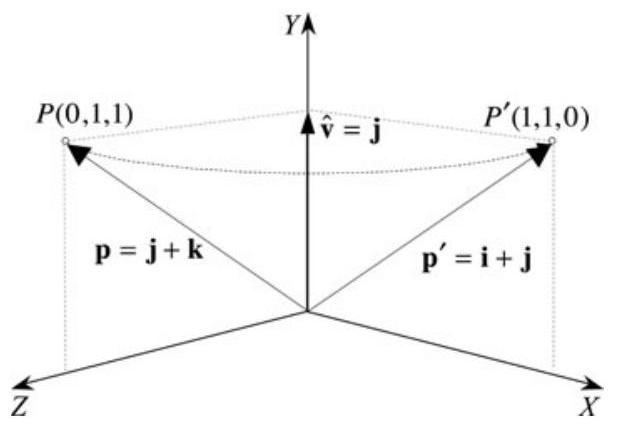
\includegraphics[max width=\textwidth]{2023_01_16_a848224efad29cd66460g-116}
\end{center}

clockwise:

$$
\begin{aligned}
q p q^{-1} & =[0,(1-\cos \theta)(\hat{\mathbf{v}} \cdot \mathbf{p}) \hat{\mathbf{v}}+\cos \theta \mathbf{p}+\sin \theta \hat{\mathbf{v}} \times \mathbf{p}] \\
q^{-1} p q & =[0,(1-\cos \theta)(\hat{\mathbf{v}} \cdot \mathbf{p}) \hat{\mathbf{v}}+\cos \theta \mathbf{p}-\sin \theta \hat{\mathbf{v}} \times \mathbf{p}]
\end{aligned}
$$

Let's compute another example. Consider the point $P(0,1,1)$ in Fig. $7.6$ which is to be rotated $90^{\circ}$ about the $y$-axis. We can see that the rotated point $P^{\prime}$ has the coordinates $(1,1,0)$ which we will confirm algebraically. The point $P$ is represented by its position vector $\mathbf{p}$ in the pure quaternion

$$
p=[0, \mathbf{p}] \text {. }
$$

The axis of rotation is $\hat{\mathbf{v}}=\mathbf{j}$, and the vector to be rotated is $\mathbf{p}=\mathbf{j}+\mathbf{k}$. Therefore,

$$
\begin{aligned}
\operatorname{qpq}^{-1} & =[0,(1-\cos \theta)(\hat{\mathbf{v}} \cdot \mathbf{p}) \hat{\mathbf{v}}+\cos \theta \mathbf{p}+\sin \theta \hat{\mathbf{v}} \times \mathbf{p}] \\
& =[0, \mathbf{j} \cdot(\mathbf{j}+\mathbf{k}) \mathbf{j}+\mathbf{j} \times(\mathbf{j}+\mathbf{k})] \\
& =[0, \mathbf{i}+\mathbf{j}]
\end{aligned}
$$

and confirms that $P$ is indeed rotated to $(1,1,0)$.

Now let's explore how this product is represented in matrix form.

\section{矩阵形式的四元数}
Having discovered a vector equation to represent the triple $q p q^{-1}$, let's continue and convert it into a matrix. We will explore two methods: the first is a simple vectorial method which translates the vector equation representing $q p q^{-1}$ directly into matrix form. The second method uses matrix algebra to develop a rather cunning solution.

\subsection{向量方法}
For the vector method it is convenient to describe the unit-norm quaternion as

$$
\begin{aligned}
q & =[s, \mathbf{v}] \\
& =[s, x \mathbf{i}+y \mathbf{j}+z \mathbf{k}]
\end{aligned}
$$

where

$$
s^{2}+|\mathbf{v}|^{2}=1
$$

and the pure quaternion as

$$
\begin{aligned}
p & =[0, \mathbf{p}] \\
& =\left[0, x_{p} \mathbf{i}+y_{p} \mathbf{j}+z_{p} \mathbf{k}\right] .
\end{aligned}
$$

A simple way to compute $q p q^{-1}$ is to use (7.11) and substitute $|\mathbf{v}|$ for $\lambda$ :

$$
\begin{aligned}
q p q^{-1} & =\left[0,2 \lambda^{2}(\hat{\mathbf{v}} \cdot \mathbf{p}) \hat{\mathbf{v}}+\left(s^{2}-\lambda^{2}\right) \mathbf{p}+2 \lambda s \hat{\mathbf{v}} \times \mathbf{p}\right] \\
& =\left[0,2|\mathbf{v}|^{2}(\hat{\mathbf{v}} \cdot \mathbf{p}) \hat{\mathbf{v}}+\left(s^{2}-|\mathbf{v}|^{2}\right) \mathbf{p}+2|\mathbf{v}| s \hat{\mathbf{v}} \times \mathbf{p}\right]
\end{aligned}
$$

Next, we substitute $\mathbf{v}$ for $|\mathbf{v}| \hat{\mathbf{v}}$ :

$$
q p q^{-1}=\left[0,2(\mathbf{v} \cdot \mathbf{p}) \mathbf{v}+\left(s^{2}-|\mathbf{v}|^{2}\right) \mathbf{p}+2 s \mathbf{v} \times \mathbf{p}\right]
$$

Finally, as we are working with unit-norm quaternions to prevent scaling

$$
s^{2}+|\mathbf{v}|^{2}=1
$$

and

$$
s^{2}-|\mathbf{v}|^{2}=2 s^{2}-1
$$

therefore,

$$
q p q^{-1}=\left[0,2(\mathbf{v} \cdot \mathbf{p}) \mathbf{v}+\left(2 s^{2}-1\right) \mathbf{p}+2 s \mathbf{v} \times \mathbf{p}\right]
$$

If we let $p^{\prime}=q p q^{-1}$, which is a pure quaternion, we have

$$
\begin{aligned}
p^{\prime} & =q p q^{-1} \\
& =\left[0, \mathbf{p}^{\prime}\right] \\
& =\left[0,2(\mathbf{v} \cdot \mathbf{p}) \mathbf{v}+\left(2 s^{2}-1\right) \mathbf{p}+2 s \mathbf{v} \times \mathbf{p}\right] \\
\mathbf{p}^{\prime} & =2(\mathbf{v} \cdot \mathbf{p}) \mathbf{v}+\left(2 s^{2}-1\right) \mathbf{p}+2 s \mathbf{v} \times \mathbf{p} .
\end{aligned}
$$

We are only interested in the rotated vector $\mathbf{p}^{\prime}$ comprising the three terms $2(\mathbf{v} \cdot \mathbf{p}) \mathbf{v}$, $\left(2 s^{2}-1\right) \mathbf{p}$ and $2 s \mathbf{v} \times \mathbf{p}$, which can be represented by three individual matrices and summed together.

$$
\begin{aligned}
2(\mathbf{v} \cdot \mathbf{p}) \mathbf{v} & =2\left(x x_{p}+y y_{p}+z z_{p}\right)(x \mathbf{i}+y \mathbf{j}+z \mathbf{k}) \\
& =\left[\begin{array}{lll}
2 x^{2} & 2 x y & 2 x z \\
2 x y & 2 y^{2} & 2 y z \\
2 x z & 2 y z & 2 z^{2}
\end{array}\right]\left[\begin{array}{l}
x_{p} \\
y_{p} \\
z_{p}
\end{array}\right] \\
\left(2 s^{2}-1\right) \mathbf{p} & =\left(2 s^{2}-1\right) x_{p} \mathbf{i}+\left(2 s^{2}-1\right) y_{p} \mathbf{j}+\left(2 s^{2}-1\right) z_{p} \mathbf{k} \\
& =\left[\begin{array}{ccc}
2 s^{2}-1 & 0 & 0 \\
0 & 2 s^{2}-1 & 0 \\
0 & 0 & 2 s^{2}-1
\end{array}\right]\left[\begin{array}{l}
x_{p} \\
y_{p} \\
z_{p}
\end{array}\right]
\end{aligned}
$$

$$
\begin{aligned}
2 s \mathbf{v} \times \mathbf{p} & =2 s\left(\left(y z_{p}-z y_{p}\right) \mathbf{i}+\left(z x_{p}-x z_{p}\right) \mathbf{j}+\left(x y_{p}-y x_{p}\right) \mathbf{k}\right) \\
& =\left[\begin{array}{ccc}
0 & -2 s z & 2 s y \\
2 s z & 0 & -2 s x \\
-2 s y & 2 s x & 0
\end{array}\right]\left[\begin{array}{l}
x_{p} \\
y_{p} \\
z_{p}
\end{array}\right] .
\end{aligned}
$$

Adding these matrices together:

$$
\mathbf{p}^{\prime}=\left[\begin{array}{ccc}
2\left(s^{2}+x^{2}\right)-1 & 2(x y-s z) & 2(x z+s y) \\
2(x y+s z) & 2\left(s^{2}+y^{2}\right)-1 & 2(y z-s x) \\
2(x z-s y) & 2(y z+s x) & 2\left(s^{2}+z^{2}\right)-1
\end{array}\right]\left[\begin{array}{l}
x_{p} \\
y_{p} \\
z_{p}
\end{array}\right]
$$

or

$$
\mathbf{p}^{\prime}=\left[\begin{array}{ccc}
1-2\left(y^{2}+z^{2}\right) & 2(x y-s z) & 2(x z+s y) \\
2(x y+s z) & 1-2\left(x^{2}+z^{2}\right) & 2(y z-s x) \\
2(x z-s y) & 2(y z+s x) & 1-2\left(x^{2}+y^{2}\right)
\end{array}\right]\left[\begin{array}{l}
x_{p} \\
y_{p} \\
z_{p}
\end{array}\right]
$$

where

$$
\left[0, \mathbf{p}^{\prime}\right]=q p q^{-1}
$$

Now let's reverse the product. To compute the vector part of $q^{-1} p q$ all that we have to do is reverse the sign of $2 s \mathbf{v} \times \mathbf{p}$ :

$$
\mathbf{p}^{\prime}=\left[\begin{array}{ccc}
2\left(s^{2}+x^{2}\right)-1 & 2(x y+s z) & 2(x z-s y) \\
2(x y-s z) & 2\left(s^{2}+y^{2}\right)-1 & 2(y z+s x) \\
2(x z+s y) & 2(y z-s x) & 2\left(s^{2}+z^{2}\right)-1
\end{array}\right]\left[\begin{array}{l}
x_{p} \\
y_{p} \\
z_{p}
\end{array}\right]
$$

or

$$
\mathbf{p}^{\prime}=\left[\begin{array}{ccc}
1-2\left(y^{2}+z^{2}\right) & 2(x y+s z) & 2(x z-s y) \\
2(x y-s z) & 1-2\left(x^{2}+z^{2}\right) & 2(y z+s x) \\
2(x z+s y) & 2(y z-s x) & 1-2\left(x^{2}+y^{2}\right)
\end{array}\right]\left[\begin{array}{l}
x_{p} \\
y_{p} \\
z_{p}
\end{array}\right]
$$

where

$$
\left[0, \mathbf{p}^{\prime}\right]=q^{-1} p q .
$$

Observe that (7.17) is the transpose of (7.15), and (7.18) is the transpose of (7.16).

\subsection{矩阵方法}
The second method to derive (7.13) employs the matrix representing a quaternion product $(5.14)$ :

$$
\begin{aligned}
q_{a} & =\left[s_{a}, x_{a} \mathbf{i}+y_{a} \mathbf{j}+z_{a} \mathbf{k}\right] \\
q_{b} & =\left[s_{b}, x_{b} \mathbf{i}+y_{b} \mathbf{j}+z_{b} \mathbf{k}\right]
\end{aligned}
$$

and their product is

$$
\begin{aligned}
& q_{a} q_{b}=\left[s_{a}, x_{a} \mathbf{i}+y_{a} \mathbf{j}+z_{a} \mathbf{k}\right]\left[s_{b}, x_{b} \mathbf{i}+y_{b} \mathbf{j}+z_{b} \mathbf{k}\right] \\
& =\left[s_{a} s_{b}-x_{a} x_{b}-y_{a} y_{b}-z_{a} z_{b},\right. \\
& s_{a}\left(x_{b} \mathbf{i}+y_{b} \mathbf{j}+z_{b} \mathbf{k}\right) \\
& +s_{b}\left(x_{a} \mathbf{i}+y_{a} \mathbf{j}+z_{a} \mathbf{k}\right) \\
& \left.+\left(y_{a} z_{b}-y_{b} z_{a}\right) \mathbf{i}+\left(x_{b} z_{a}-x_{a} z_{b}\right) \mathbf{j}+\left(x_{a} y_{b}-x_{b} y_{a}\right) \mathbf{k}\right] \\
& =\left[s_{a} s_{b}-x_{a} x_{b}-y_{a} y_{b}-z_{a} z_{b}\right. \text {, } \\
& \left(s_{a} x_{b}+s_{b} x_{a}+y_{a} z_{b}-y_{b} z_{a}\right) \mathbf{i} \\
& +\left(s_{a} y_{b}+s_{b} y_{a}+x_{b} z_{a}-x_{a} z_{b}\right) \mathbf{j} \\
& \left.+\left(s_{a} z_{b}+s_{b} z_{a}+x_{a} y_{b}-x_{b} y_{a}\right) \mathbf{k}\right] \\
& =\left[\begin{array}{cccc}s_{a} & -x_{a} & -y_{a} & -z_{a} \\x_{a} & s_{a} & -z_{a} & y_{a} \\y_{a} & z_{a} & s_{a} & -x_{a} \\z_{a} & -y_{a} & x_{a} & s_{a}\end{array}\right]\left[\begin{array}{c}s_{b} \\x_{b} \\y_{b} \\z_{b}\end{array}\right]=\mathbf{A} q_{b} .
\end{aligned}
$$

At this stage we have quaternion $q_{a}$ represented by matrix $\mathbf{A}$, and quaternion $q_{b}$ represented as a column vector. Now let's reverse the scenario without altering the result by making $q_{b}$ the matrix and $q_{a}$ the column vector:

$$
q_{a} q_{b}=\left[\begin{array}{cccc}
s_{b} & -x_{b} & -y_{b} & -z_{b} \\
x_{b} & s_{b} & z_{b} & -y_{b} \\
y_{b} & -z_{b} & s_{b} & x_{b} \\
z_{b} & y_{b} & -x_{b} & s_{b}
\end{array}\right]\left[\begin{array}{c}
s_{a} \\
x_{a} \\
y_{a} \\
z_{a}
\end{array}\right]=\mathbf{B} q_{a}
$$

So now we have two ways of computing $q_{a} q_{b}$ and we need a way of distinguishing between the two matrices. Let $\mathbf{L}$ be the matrix that preserves the left-to-right quaternion sequence, and $\mathbf{R}$ be the matrix that reverses the sequence to right-to-left:

$$
\begin{aligned}
& q_{a} q_{b}=\mathbf{L}\left(q_{a}\right) q_{b}= {\left[\begin{array}{cccc}
s_{a} & -x_{a} & -y_{a} & -z_{a} \\
x_{a} & s_{a} & -z_{a} & y_{a} \\
y_{a} & z_{a} & s_{a} & -x_{a} \\
z_{a} & -y_{a} & x_{a} & s_{a}
\end{array}\right]\left[\begin{array}{c}
s_{b} \\
x_{b} \\
y_{b} \\
z_{b}
\end{array}\right] } \\
& q_{a} q_{b}=\mathbf{R}\left(q_{b}\right) q_{a}=\left[\begin{array}{cccc}
s_{b} & -x_{b} & -y_{b} & -z_{b} \\
x_{b} & s_{b} & z_{b} & -y_{b} \\
y_{b} & -z_{b} & s_{b} & x_{b} \\
z_{b} & y_{b} & -x_{b} & s_{b}
\end{array}\right]\left[\begin{array}{c}
s_{a} \\
x_{a} \\
y_{a} \\
z_{a}
\end{array}\right] .
\end{aligned}
$$

Remember that $\mathbf{L}\left(q_{a}\right) q_{b}=\mathbf{R}\left(q_{b}\right) q_{a}$, as this is central to understanding the next stage. Furthermore, don't be surprised if you can't follow the argument in the first reading. It took the author many hours of anguish trying to decipher the original algorithm, and this explanation has been expanded to ensure that you do not suffer the same experience!

First, let's employ the matrices $\mathbf{L}$ and $\mathbf{R}$ to rearrange the quaternion product $q_{a} q_{c} q_{b}$ to $q_{a} q_{b} q_{c}$, i.e. move $q_{c}$ from the middle to the right-hand-side. We start with the quaternion product $q_{a} q_{c} q_{b}$ and divide it into two parts, $q_{a} q_{c}$ and $q_{b}$. We can do this because quaternion algebra is associative:

$$
q_{a} q_{c} q_{b}=\left(q_{a} q_{c}\right) q_{b}
$$

We have already demonstrated above that the product $q_{a} q_{c}$ can be replaced by $\mathbf{L}\left(q_{a}\right) q_{c}$

$$
q_{a} q_{c} q_{b}=\mathbf{L}\left(q_{a}\right) q_{c} q_{b}
$$

We now have another two parts: $\mathbf{L}\left(q_{a}\right) q_{c}$ and $q_{b}$ which can be reversed using $\mathbf{R}$ without disturbing the result:

$$
q_{a} q_{c} q_{b}=\mathbf{L}\left(q_{a}\right) q_{c} q_{b}=\mathbf{R}\left(q_{b}\right) \mathbf{L}\left(q_{a}\right) q_{c}
$$

which has achieved our objective to move $q_{c}$ to the right-hand-side. But the most important result is that the matrices $\mathbf{R}\left(q_{b}\right)$ and $\mathbf{L}\left(q_{a}\right)$ can be multiplied together to form a single matrix, which operates on $q_{c}$.

Now let's repeat the same process to rearrange the product $q p q^{-1}$. The objective is to move $p$ from the middle of $q$ and $q^{-1}$, to the right-hand-side. The reason for doing this is to bring together $q$ and $q^{-1}$ in the form of two matrices, which can be multiplied together into a single matrix.

We start with the quaternion product $q p q^{-1}$ and divide it into two parts, $q p$ and $q^{-1}$

$$
q p q^{-1}=(q p) q^{-1}
$$

The product $q p$ can be replaced by $\mathbf{L}(q) p$ :

$$
q p q^{-1}=\mathbf{L}(q) p q^{-1}
$$

We now have another two parts: $\mathbf{L}(q) p$ and $q^{-1}$ which can be reversed using $\mathbf{R}$ without disturbing the result:

$$
q p q^{-1}=\mathbf{L}(q) p q^{-1}=\mathbf{R}\left(q^{-1}\right) \mathbf{L}(q) p
$$

which has achieved our objective to move $p$ to the right-hand-side.

The next step is to compute $\mathbf{L}(q)$ and $\mathbf{R}\left(q^{-1}\right)$ using $q=[s, x \mathbf{i}+y \mathbf{j}+z \mathbf{k}]$.

$\mathbf{L}(q)$ is easy as it is the same as $\mathbf{L}\left(q_{a}\right)$ :

$$
\mathbf{L}(q)=\left[\begin{array}{cccc}
s & -x & -y & -z \\
x & s & -z & y \\
y & z & s & -x \\
z & -y & x & s
\end{array}\right]
$$

$\mathbf{R}\left(q^{-1}\right)$ is also easy, but requires converting $q_{b}$ in the original definition into $q^{-1}$ which is effected by reversing the signs of the vector components:

$$
\mathbf{R}\left(q^{-1}\right)=\left[\begin{array}{cccc}
s & x & y & z \\
-x & s & -z & y \\
-y & z & s & -x \\
-z & -y & x & s
\end{array}\right]
$$

Fig. 7.7 The point $P(0,1,1)$ is rotated $90^{\circ}$ to $P^{\prime}(1,1,0)$ about the $y$-axis

\begin{center}
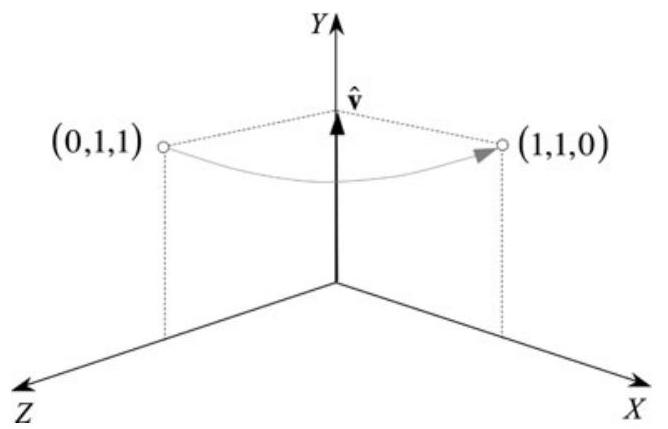
\includegraphics[max width=\textwidth]{2023_01_16_a848224efad29cd66460g-121}
\end{center}

So now we can write

$$
\begin{aligned}
q p q^{-1} & =\mathbf{R}\left(q^{-1}\right) \mathbf{L}(q) p \\
& =\left[\begin{array}{cccc}
s & x & y & z \\
-x & s & -z & y \\
-y & z & s & -x \\
-z & -y & x & s
\end{array}\right]\left[\begin{array}{cccc}
s & -x & -y & -z \\
x & s & -z & y \\
y & z & s & -x \\
z & -y & x & s
\end{array}\right]\left[\begin{array}{c}
0 \\
x_{p} \\
y_{p} \\
z_{p}
\end{array}\right] \\
& =\left[\begin{array}{cccc}
1 & 0 & 0 & 0 \\
0 & 1-2\left(y^{2}+z^{2}\right) & 2(x y-s z) & 2(x z+s y) \\
0 & 2(x y+s z) & 1-2\left(x^{2}+z^{2}\right) & 2(y z-s x) \\
0 & 2(x z-s y) & 2(y z+s x) & 1-2\left(x^{2}+y^{2}\right)
\end{array}\right]\left[\begin{array}{c}
0 \\
x_{p} \\
y_{p} \\
z_{p}
\end{array}\right] .
\end{aligned}
$$

If we ignore the first row and column, the matrix computes $\mathbf{p}^{\prime}$ :

$$
\mathbf{p}^{\prime}=\left[\begin{array}{ccc}
1-2\left(y^{2}+z^{2}\right) & 2(x y-s z) & 2(x z+s y) \\
2(x y+s z) & 1-2\left(x^{2}+z^{2}\right) & 2(y z-s x) \\
2(x z-s y) & 2(y z+s x) & 1-2\left(x^{2}+y^{2}\right)
\end{array}\right]\left[\begin{array}{l}
x_{p} \\
y_{p} \\
z_{p}
\end{array}\right]
$$

which is identical to (7.16)!

\subsection{几何验证}
Let's illustrate the action of (7.15) by rotating the point $(0,1,1), 90^{\circ}$ about the $y$ axis, as shown in Fig. 7.7. The quaternion takes the form

$$
q=\left[\cos \frac{1}{2} \theta, \sin \frac{1}{2} \theta \hat{\mathbf{v}}\right]
$$

which means that $\theta=90^{\circ}$ and $\hat{\mathbf{v}}=\mathbf{j}$, therefore,

$$
q=\left[\cos 45^{\circ}, \sin 45^{\circ} \hat{\mathbf{j}}\right]
$$

Consequently,

$$
s=\frac{\sqrt{2}}{2}, \quad x=0, \quad y=\frac{\sqrt{2}}{2}, \quad z=0 .
$$

Substituting these values in (7.15) gives

$$
\begin{aligned}
\mathbf{p}^{\prime} & =\left[\begin{array}{ccc}
2\left(s^{2}+x^{2}\right)-1 & 2(x y-s z) & 2(x z+s y) \\
2(x y+s z) & 2\left(s^{2}+y^{2}\right)-1 & 2(y z-s x) \\
2(x z-s y) & 2(y z+s x) & 2\left(s^{2}+z^{2}\right)-1
\end{array}\right]\left[\begin{array}{l}
x_{p} \\
y_{p} \\
z_{p}
\end{array}\right] \\
{\left[\begin{array}{l}
1 \\
1 \\
0
\end{array}\right] } & =\left[\begin{array}{ccc}
0 & 0 & 1 \\
0 & 1 & 0 \\
-1 & 0 & 0
\end{array}\right]\left[\begin{array}{l}
0 \\
1 \\
1
\end{array}\right]
\end{aligned}
$$

where $(0,1,1)$ is rotated to $(1,1,0)$, which is correct.

So now we have a transform that rotates a point about an arbitrary axis intersecting the origin without the problems of gimbal lock associated with Euler transforms.

Before moving on, let's evaluate one more example. Let's perform a $180^{\circ}$ rotation about a vector $\mathbf{v}=\mathbf{i}+\mathbf{k}$ passing through the origin. To begin with, we will deliberately forget to convert the vector into a unit vector, just to see what happens to the final matrix. The quaternion takes the form

$$
q=\left[\cos \frac{1}{2} \theta, \sin \frac{1}{2} \theta \hat{\mathbf{v}}\right]
$$

but we will use $\mathbf{v}$ as specified. Therefore, with $\theta=180^{\circ}$

$$
s=0, \quad x=1, \quad y=0, \quad z=1 .
$$

Substituting these values in (7.15) gives

$$
\begin{aligned}
\mathbf{p}^{\prime} & =\left[\begin{array}{ccc}
2\left(s^{2}+x^{2}\right)-1 & 2(x y-s z) & 2(x z+s y) \\
2(x y+s z) & 2\left(s^{2}+y^{2}\right)-1 & 2(y z-s x) \\
2(x z-s y) & 2(y z+s x) & 2\left(s^{2}+z^{2}\right)-1
\end{array}\right]\left[\begin{array}{l}
x_{p} \\
y_{p} \\
z_{p}
\end{array}\right] \\
& =\left[\begin{array}{ccc}
1 & 0 & 2 \\
0 & -1 & 0 \\
2 & 0 & 1
\end{array}\right]\left[\begin{array}{l}
1 \\
0 \\
0
\end{array}\right]
\end{aligned}
$$

which looks nothing like a rotation matrix, and reminds us how important it is to have a unit vector to represent the axis. Let's repeat these calculations normalising the vector to $\hat{\mathbf{v}}=\frac{1}{\sqrt{2}} \mathbf{i}+\frac{1}{\sqrt{2}} \mathbf{k}$ :

$$
s=0, \quad x=\frac{1}{\sqrt{2}}, \quad y=0, \quad z=\frac{1}{\sqrt{2}} .
$$

Substituting these values in (7.15) gives

$$
\begin{aligned}
\mathbf{p}^{\prime} & =\left[\begin{array}{ccc}
2\left(s^{2}+x^{2}\right)-1 & 2(x y-s z) & 2(x z+s y) \\
2(x y+s z) & 2\left(s^{2}+y^{2}\right)-1 & 2(y z-s x) \\
2(x z-s y) & 2(y z+s x) & 2\left(s^{2}+z^{2}\right)-1
\end{array}\right]\left[\begin{array}{l}
x_{p} \\
y_{p} \\
z_{p}
\end{array}\right] \\
{\left[\begin{array}{l}
0 \\
0 \\
1
\end{array}\right] } & =\left[\begin{array}{ccc}
0 & 0 & 1 \\
0 & -1 & 0 \\
1 & 0 & 0
\end{array}\right]\left[\begin{array}{l}
1 \\
0 \\
0
\end{array}\right]
\end{aligned}
$$

Fig. 7.8 The point $(1,0,0)$ is rotated $180^{\circ}$ about the vector $\hat{\mathbf{v}}$ to $(0,0,1)$

\begin{center}
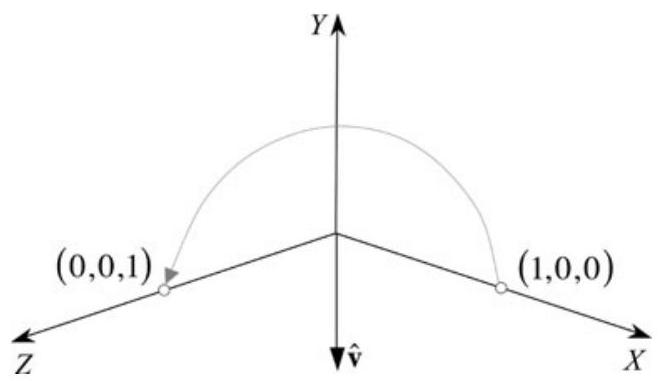
\includegraphics[max width=\textwidth]{2023_01_16_a848224efad29cd66460g-123}
\end{center}

which not only looks like a rotation matrix, but has a determinant of 1 and rotates the point $(1,0,0)$ to $(0,0,1)$ as shown in Fig. 7.8.

\section{多个旋转}
Say a vector or frame of reference is subjected to two rotations specified by $q_{1}$ followed by $q_{2}$. There is a temptation to convert both quaternions to their respective matrix and multiply the matrices together. However, this not the most efficient way of combining the rotations. It is best to accumulate the rotations as quaternions and then convert to matrix notation, if required.

To illustrate this, consider the pure quaternion $p$ subjected to the first quaternion $q_{1}$ :

$$
q_{1} p q_{1}^{-1}
$$

followed by a second quaternion $q_{2}$

$$
q_{2}\left(q_{1} p q_{1}^{-1}\right) q_{2}^{-1}
$$

which can be expressed as

$$
\left(q_{2} q_{1}\right) p\left(q_{2} q_{1}\right)^{-1} .
$$

Extra quaternions can be added accordingly. Let's illustrate this with two examples.

To keep things simple, the first quaternion $q_{1}$ rotates $30^{\circ}$ about the $y$-axis:

$$
q_{1}=\left[\cos 15^{\circ}, \sin 15^{\circ} \mathbf{j}\right] .
$$

The second quaternion $q_{2}$ rotates $60^{\circ}$ also about the $y$-axis:

$$
q_{2}=\left[\cos 30^{\circ}, \sin 30^{\circ} \mathbf{j}\right] .
$$

Together, the two quaternions rotate $90^{\circ}$ about the $y$-axis. To accumulate these rotations, we multiply them together:

$$
\begin{aligned}
q_{1} q_{2} & =\left[\cos 15^{\circ}, \sin 15^{\circ} \mathbf{j}\right]\left[\cos 30^{\circ}, \sin 30^{\circ} \mathbf{j}\right] \\
& =\left[\cos 15^{\circ} \cos 30^{\circ}-\sin 15^{\circ} \sin 30^{\circ}, \cos 15^{\circ} \sin 30^{\circ} \mathbf{j}+\cos 30^{\circ} \sin 15^{\circ} \mathbf{j}\right] \\
& =\left[\frac{\sqrt{2}}{2}, \frac{\sqrt{2}}{2} \mathbf{j}\right]
\end{aligned}
$$

which is a quaternion that rotates $90^{\circ}$ about the $y$-axis. Using the matrix (7.15) we have

$$
\begin{aligned}
\mathbf{p}^{\prime} & =\left[\begin{array}{ccc}
2\left(s^{2}+x^{2}\right)-1 & 2(x y-s z) & 2(x z+s y) \\
2(x y+s z) & 2\left(s^{2}+y^{2}\right)-1 & 2(y z-s x) \\
2(x z-s y) & 2(y z+s x) & 2\left(s^{2}+z^{2}\right)-1
\end{array}\right]\left[\begin{array}{l}
x_{p} \\
y_{p} \\
z_{p}
\end{array}\right] \\
& =\left[\begin{array}{ccc}
0 & 0 & 1 \\
0 & 1 & 0 \\
-1 & 0 & 0
\end{array}\right]\left[\begin{array}{c}
x_{p} \\
y_{p} \\
z_{p}
\end{array}\right]
\end{aligned}
$$

which rotates points about the $y$-axis by $90^{\circ}$.

For a second example, let's just evaluate the quaternions. The first quaternion $q_{1}$ rotates $90^{\circ}$ about the $x$-axis, and $q_{2}$ rotates $90^{\circ}$ about the $y$-axis:

$$
\begin{aligned}
q_{1} & =\left[\frac{\sqrt{2}}{2}, \frac{\sqrt{2}}{2} \mathbf{i}\right] \\
q_{2} & =\left[\frac{\sqrt{2}}{2}, \frac{\sqrt{2}}{2} \mathbf{j}\right] \\
p & =[0, \mathbf{i}+\mathbf{j}]
\end{aligned}
$$

therefore,

$$
\begin{aligned}
q_{2} q_{1} & =\left[\frac{\sqrt{2}}{2}, \frac{\sqrt{2}}{2} \mathbf{j}\right]\left[\frac{\sqrt{2}}{2}, \frac{\sqrt{2}}{2} \mathbf{i}\right] \\
& =\left[\frac{1}{2}, \frac{\sqrt{2}}{2} \frac{\sqrt{2}}{2} \mathbf{i}+\frac{\sqrt{2}}{2} \frac{\sqrt{2}}{2} \mathbf{j}-\frac{1}{2} \mathbf{k}\right] \\
& =\left[\frac{1}{2}, \frac{1}{2} \mathbf{i}+\frac{1}{2} \mathbf{j}-\frac{1}{2} \mathbf{k}\right] \\
\left(q_{2} q_{1}\right)^{-1} & =\left[\frac{1}{2},-\frac{1}{2} \mathbf{i}-\frac{1}{2} \mathbf{j}+\frac{1}{2} \mathbf{k}\right] \\
\left(q_{2} q_{1}\right) p & =\left[\frac{1}{2}, \frac{1}{2} \mathbf{i}+\frac{1}{2} \mathbf{j}-\frac{1}{2} \mathbf{k}\right][0, \mathbf{i}+\mathbf{j}] \\
& =\left[-\frac{1}{2}-\frac{1}{2}, \frac{1}{2}(\mathbf{i}+\mathbf{j})+\frac{1}{2} \mathbf{i}-\frac{1}{2} \mathbf{j}\right] \\
& =[-1, \mathbf{i}] \\
\left(q_{2} q_{1}\right) p\left(q_{2} q_{1}\right)^{-1} & =[-1, \mathbf{i}]\left[\frac{1}{2},-\frac{1}{2} \mathbf{i}-\frac{1}{2} \mathbf{j}+\frac{1}{2} \mathbf{k}\right] \\
& =\left[-\frac{1}{2}+\frac{1}{2}, \frac{1}{2} \mathbf{i}+\frac{1}{2} \mathbf{j}-\frac{1}{2} \mathbf{k}+\frac{1}{2} \mathbf{i}-\frac{1}{2} \mathbf{j}-\frac{1}{2} \mathbf{k}\right] \\
& =[0, \mathbf{i}-\mathbf{k}] .
\end{aligned}
$$

Thus the point $(1,1,0)$ is rotated to $(1,0,-1)$, which is correct.

\section{特征值和特征向量}
Although there is no doubt that (7.15) is a rotation matrix, we can secure further evidence by calculating its eigenvalue and eigenvector. The eigenvalue should be $\theta$ where

$$
\operatorname{Tr}\left(q p q^{-1}\right)=1+2 \cos \theta
$$

and $\operatorname{Tr}$ is the trace function, which is the sum of the diagonal elements of a matrix.

The trace of $(7.15)$ is

$$
\begin{aligned}
\operatorname{Tr}\left(q p q^{-1}\right) & =2\left(s^{2}+x^{2}\right)-1+2\left(s^{2}+y^{2}\right)-1+2\left(s^{2}+z^{2}\right)-1 \\
& =4 s^{2}+2\left(s^{2}+x^{2}+y^{2}+z^{2}\right)-3 \\
& =4 s^{2}-1 \\
& =4 \cos ^{2} \frac{1}{2} \theta-1 \\
& =4 \cos \theta+4 \sin ^{2} \frac{1}{2} \theta-1 \\
& =4 \cos \theta+2-2 \cos \theta-1 \\
& =1+2 \cos \theta
\end{aligned}
$$

and

$$
\cos \theta=\frac{1}{2}\left(\operatorname{Tr}\left(q p q^{-1}\right)-1\right) .
$$

To compute the eigenvector of (7.15) we use the three equations derived in Appendix:

$$
\begin{aligned}
& x_{v}=\left(a_{22}-1\right)\left(a_{33}-1\right)-a_{23} a_{32} \\
& y_{v}=\left(a_{33}-1\right)\left(a_{11}-1\right)-a_{31} a_{13} \\
& z_{v}=\left(a_{11}-1\right)\left(a_{22}-1\right)-a_{12} a_{21} .
\end{aligned}
$$

Therefore,

$$
\begin{aligned}
x_{v} & =\left(2\left(s^{2}+y^{2}\right)-2\right)\left(2\left(s^{2}+z^{2}\right)-2\right)-2(y z-s x) 2(y z+s x) \\
& =4\left(s^{2}+y^{2}-1\right)\left(s^{2}+z^{2}-1\right)-4\left(y^{2} z^{2}-s^{2} x^{2}\right) \\
& =4\left(\left(x^{2}+z^{2}\right)\left(x^{2}+y^{2}\right)-y^{2} z^{2}+s^{2} x^{2}\right) \\
& =4\left(x^{4}+x^{2} y^{2}+x^{2} z^{2}+z^{2} y^{2}-y^{2} z^{2}+s^{2} x^{2}\right) \\
& =4 x^{2}\left(s^{2}+x^{2}+y^{2}+z^{2}\right) \\
& =4 x^{2} .
\end{aligned}
$$

Similarly, $y_{v}=4 y^{2}$ and $z_{v}=4 z^{2}$, which confirm that the eigenvector has components associated with the quaternion's vector. The square terms should be no surprise, as the triple $q p q^{-1}$ includes the product of three quaternions. Let's test these formulae with the matrix associated with Fig. 7.8, which rotates a point $180^{\circ}$ about the vector $\hat{\mathbf{v}}=\frac{1}{\sqrt{2}} \mathbf{i}+\frac{1}{\sqrt{2}} \mathbf{k}$ :

$$
\mathbf{M}=\left[\begin{array}{lll}
a_{11} & a_{12} & a_{13} \\
a_{21} & a_{22} & a_{23} \\
a_{31} & a_{32} & a_{33}
\end{array}\right]=\left[\begin{array}{ccc}
0 & 0 & 1 \\
0 & -1 & 0 \\
1 & 0 & 0
\end{array}\right]
$$

therefore,

$$
\begin{aligned}
& x_{v}=-2 \times-1-0=2 \\
& y_{v}=-1 \times-1-1 \times 1=0 \\
& z_{v}=-1 \times-2-0=2
\end{aligned}
$$

which confirms that the eigenvector is $2 \mathbf{i}+2 \mathbf{k}$.

Next, $\operatorname{Tr}(\mathbf{M})=-1$, therefore

$$
\begin{aligned}
\cos \theta & =\frac{1}{2}\left(\operatorname{Tr}\left(q p q^{-1}\right)-1\right) \\
& =\frac{1}{2}((-1)-1) \\
& =-1 \\
\theta & =\pm 180^{\circ}
\end{aligned}
$$

which agrees with the previous results.

\section{绕偏移轴旋转}
Now that we have a matrix to represent a quaternion rotor, we can employ it to resolve problems such as rotating a point about an off-set axis using the same techniques associated with normal rotation transforms. For example, in Chap. 6 we used the following notation

$$
\left[\begin{array}{c}
x^{\prime} \\
y^{\prime} \\
z^{\prime} \\
1
\end{array}\right]=\mathbf{T}_{t_{x}, 0, t_{z}} \mathbf{R}_{\beta, y} \mathbf{T}_{-t_{x}, 0,-t_{z}}\left[\begin{array}{c}
x \\
y \\
z \\
1
\end{array}\right]
$$

to rotate a point about a fixed axis parallel with the $y$-axis. Therefore, by substituting the matrix $q p q^{-1}$ for $\mathbf{R}_{\beta, y}$ we have

$$
\left[\begin{array}{c}
x^{\prime} \\
y^{\prime} \\
z^{\prime} \\
1
\end{array}\right]=\mathbf{T}_{t_{x}, 0, t_{z}}\left(q p q^{-1}\right) \mathbf{T}_{-t_{x}, 0,-t_{z}}\left[\begin{array}{c}
x \\
y \\
z \\
1
\end{array}\right] .
$$

Let's test this by rotating our unit cube $90^{\circ}$ about the vertical axis intersecting vertices 4 and 6 as shown in Fig. 7.9. (a)

\begin{center}
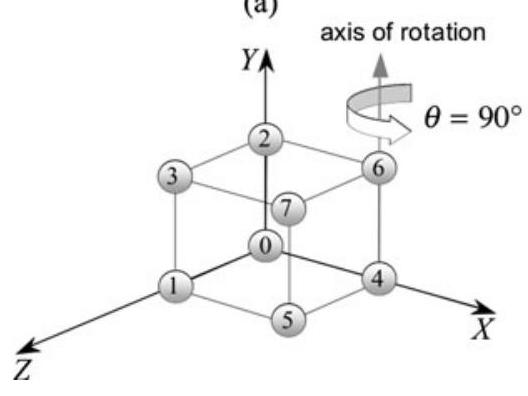
\includegraphics[max width=\textwidth]{2023_01_16_a848224efad29cd66460g-127}
\end{center}

(b)

\begin{center}
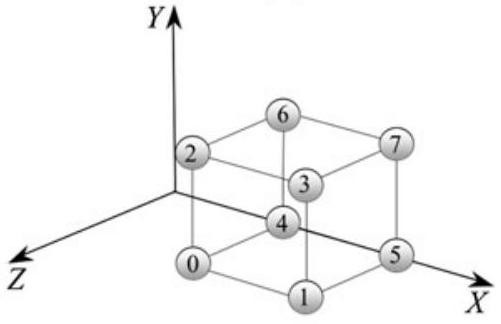
\includegraphics[max width=\textwidth]{2023_01_16_a848224efad29cd66460g-127(1)}
\end{center}

Fig. 7.9 The cube is rotated $90^{\circ}$ about the axis intersecting vertices 4 and 6

The unit-norm quaternion to achieve this is

$$
q=\left[\cos 45^{\circ}, \sin 45^{\circ} \mathbf{j}\right]
$$

with the pure quaternion

$$
p=[0, \mathbf{p}]
$$

Consequently,

$$
s=\frac{\sqrt{2}}{2}, \quad x=0, \quad y=\frac{\sqrt{2}}{2}, \quad z=0
$$

and using (7.15) in a homogeneous form we have

$$
\begin{aligned}
\mathbf{p}^{\prime} & =\left[\begin{array}{cccc}
2\left(s^{2}+x^{2}\right)-1 & 2(x y-s z) & 2(x z+s y) & 0 \\
2(x y+s z) & 2\left(s^{2}+y^{2}\right)-1 & 2(y z-s x) & 0 \\
2(x z-s y) & 2(y z+s x) & 2\left(s^{2}+z^{2}\right)-1 & 0 \\
0 & 0 & 1
\end{array}\right]\left[\begin{array}{c}
x_{p} \\
y_{p} \\
z_{p} \\
1
\end{array}\right] \\
& =\left[\begin{array}{cccc}
0 & 0 & 1 & 0 \\
0 & 1 & 0 & 0 \\
-1 & 0 & 0 & 0 \\
0 & 0 & 0 & 1
\end{array}\right]\left[\begin{array}{c}
x_{p} \\
y_{p} \\
z_{p} \\
1
\end{array}\right]
\end{aligned}
$$

The other two matrices are

$$
\begin{aligned}
\mathbf{T}_{-t_{x}, 0,0} & =\left[\begin{array}{cccc}
1 & 0 & 0 & -1 \\
0 & 1 & 0 & 0 \\
0 & 0 & 1 & 0 \\
0 & 0 & 0 & 1
\end{array}\right] \\
\mathbf{T}_{t_{x}, 0,0} & =\left[\begin{array}{llll}
1 & 0 & 0 & 1 \\
0 & 1 & 0 & 0 \\
0 & 0 & 1 & 0 \\
0 & 0 & 0 & 1
\end{array}\right] .
\end{aligned}
$$

Multiplying these three matrices together creates

$$
\left[\begin{array}{cccc}
0 & 0 & 1 & 1 \\
0 & 1 & 0 & 0 \\
-1 & 0 & 0 & 1 \\
0 & 0 & 0 & 1
\end{array}\right]
$$

Although not mathematically correct, the following statement shows the matrix (7.19) and the array of coordinates representing a unit cube, followed by the rotated cube's coordinates.

$$
\begin{gathered}
{\left[\begin{array}{cccc}
0 & 0 & 1 & 1 \\
0 & 1 & 0 & 0 \\
-1 & 0 & 0 & 1 \\
0 & 0 & 0 & 1
\end{array}\right]\left[\begin{array}{llllllll}
0 & 0 & 0 & 0 & 1 & 1 & 1 & 1 \\
0 & 0 & 1 & 1 & 0 & 0 & 1 & 1 \\
0 & 1 & 0 & 1 & 0 & 1 & 0 & 1 \\
1 & 1 & 1 & 1 & 1 & 1 & 1 & 1
\end{array}\right]} \\
=\left[\begin{array}{llllllll}
1 & 2 & 1 & 2 & 1 & 2 & 1 & 2 \\
0 & 0 & 1 & 1 & 0 & 0 & 1 & 1 \\
1 & 1 & 1 & 1 & 0 & 0 & 0 & 0 \\
1 & 1 & 1 & 1 & 1 & 1 & 1 & 1
\end{array}\right]
\end{gathered}
$$

These coordinates are confirmed by Fig. 7.9.

\section{参考系}
The product $q p q^{-1}$ is used for rotating points about the vector associated with the quaternion $q$, whereas the triple $q^{-1} p q$ can be used for rotating points about the same vector in the opposite direction. But this reverse rotation is also equivalent to a change of frame of reference. To demonstrate this, consider the problem of rotating the frame of reference $180^{\circ}$ about $\mathbf{i}+\mathbf{k}$ as shown in Fig. 7.10. The unitnorm quaternion for such a rotation is

$$
\begin{aligned}
q & =\left[\cos 90^{\circ}, \sin 90^{\circ}\left(\frac{1}{\sqrt{2}} \mathbf{i}+\frac{1}{\sqrt{2}} \mathbf{k}\right)\right] \\
& =\left[0, \frac{\sqrt{2}}{2} \mathbf{i}+\frac{\sqrt{2}}{2} \mathbf{k}\right] .
\end{aligned}
$$

Consequently,

$$
s=0, \quad x=\frac{\sqrt{2}}{2}, \quad y=0, \quad z=\frac{\sqrt{2}}{2} .
$$

Substituting these values in (7.17) we obtain

$$
\begin{aligned}
q^{-1} p q & =\left[\begin{array}{ccc}
2\left(s^{2}+x^{2}\right)-1 & 2(x y+s z) & 2(x z-s y) \\
2(x y-s z) & 2\left(s^{2}+y^{2}\right)-1 & 2(y z+s x) \\
2(x z+s y) & 2(y z-s x) & 2\left(s^{2}+z^{2}\right)-1
\end{array}\right]\left[\begin{array}{l}
x_{p} \\
y_{p} \\
z_{p}
\end{array}\right] \\
& =\left[\begin{array}{ccc}
0 & 0 & 1 \\
0 & -1 & 0 \\
1 & 0 & 0
\end{array}\right]\left[\begin{array}{l}
x_{p} \\
y_{p} \\
z_{p}
\end{array}\right]
\end{aligned}
$$

(a)

\begin{center}
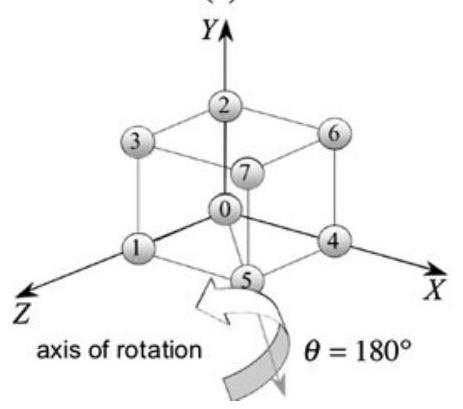
\includegraphics[max width=\textwidth]{2023_01_16_a848224efad29cd66460g-129}
\end{center}

(b)

\begin{center}
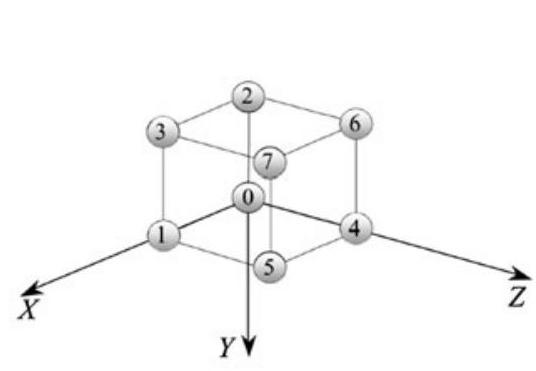
\includegraphics[max width=\textwidth]{2023_01_16_a848224efad29cd66460g-129(1)}
\end{center}

Fig. 7.10 The frame is rotated $180^{\circ}$ about the vector $\mathbf{i}+\mathbf{k}$

which, if used to process the coordinates of our unit cube, produces

$$
\begin{gathered}
{\left[\begin{array}{ccc}
0 & 0 & 1 \\
0 & -1 & 0 \\
1 & 0 & 0
\end{array}\right]\left[\begin{array}{cccccccc}
0 & 0 & 0 & 0 & 1 & 1 & 1 & 1 \\
0 & 0 & 1 & 1 & 0 & 0 & 1 & 1 \\
0 & 1 & 0 & 1 & 0 & 1 & 0 & 1
\end{array}\right]} \\
=\left[\begin{array}{cccccccc}
0 & 1 & 0 & 1 & 0 & 1 & 0 & 1 \\
0 & 0 & -1 & -1 & 0 & 0 & -1 & -1 \\
0 & 0 & 0 & 0 & 1 & 1 & 1 & 1
\end{array}\right] .
\end{gathered}
$$

This scenario is shown in Fig. $7.10$.

\section{插值四元数}
Like vectors, quaternions can be interpolated to compute an in-between quaternion. However, whereas two interpolated vectors results in a third vector that is readily visualised, two interpolated quaternions results in a third quaternion that acts as a rotor, and is not immediately visualised.

The spherical interpolant for vectors is

$$
\mathbf{v}=\frac{\sin (1-t) \theta}{\sin \theta} \mathbf{v}_{1}+\frac{\sin t \theta}{\sin \theta} \mathbf{v}_{2}
$$

where $\theta$ is the angle between the vectors, and requires no modification for quaternions:

$$
q=\frac{\sin (1-t) \theta}{\sin \theta} q_{1}+\frac{\sin t \theta}{\sin \theta} q_{2}
$$

So, given

$$
\begin{aligned}
& q_{1}=\left[s_{1}, x_{1} \mathbf{i}+y_{1} \mathbf{j}+z_{1} \mathbf{k}\right] \\
& q_{2}=\left[s_{2}, x_{2} \mathbf{i}+y_{2} \mathbf{j}+z_{2} \mathbf{k}\right]
\end{aligned}
$$

$\theta$ is obtained by taking the 4D dot product of $q_{1}$ and $q_{2}$ : Fig. 7.11 The point $(0,1,1)$ is rotated $90^{\circ}$ about the vector $\mathbf{v}_{1}$ to $(1,1,0)$
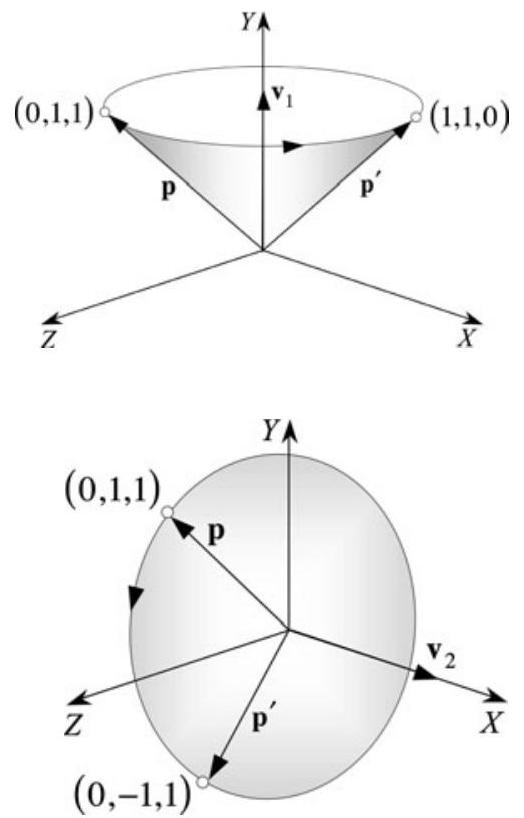
\includegraphics[max width=\textwidth, center]{2023_01_16_a848224efad29cd66460g-130}

Fig. 7.12 The point $(0,1,1)$ is rotated $90^{\circ}$ about the vector $\mathbf{v}_{2}$ to $(0,-1,1)$

$$
\begin{aligned}
\cos \theta & =\frac{q_{1} \cdot q_{2}}{\left|q_{1}\right|\left|q_{2}\right|} \\
& =\frac{s_{1} s_{2}+x_{1} x_{2}+y_{1} y_{2}+z_{1} z_{2}}{\left|q_{1}\right|\left|q_{2}\right|}
\end{aligned}
$$

and if we are working with unit-norm quaternions, then

$$
\cos \theta=s_{1} s_{2}+x_{1} x_{2}+y_{1} y_{2}+z_{1} z_{2} .
$$

Let's use (7.20) in a scenario with two simple unit-norm quaternions.

Figure $7.11$ shows one such scenario where the point $(0,1,1)$ is rotated $90^{\circ}$ about $\mathbf{v}_{1}$, the axis of $q_{1}$. Figure $7.12$ shows another scenario where the same point $(0,1,1)$ is rotated $90^{\circ}$ about $\mathbf{v}_{2}$, the axis of $q_{2}$. The quaternions are

$$
\begin{aligned}
& q_{1}=\left[\cos 45^{\circ}, \sin 45^{\circ} \mathbf{j}\right]=\left[\frac{\sqrt{2}}{2}, \frac{\sqrt{2}}{2} \mathbf{j}\right] \\
& q_{2}=\left[\cos 45^{\circ}, \sin 45^{\circ} \mathbf{i}\right]=\left[\frac{\sqrt{2}}{2}, \frac{\sqrt{2}}{2} \mathbf{i}\right] .
\end{aligned}
$$

Therefore, using (7.21)

$$
\begin{aligned}
\cos \theta & =\frac{\sqrt{2}}{2} \frac{\sqrt{2}}{2}=0.5 \\
\theta & =60^{\circ} .
\end{aligned}
$$

Before proceeding, let's compute the matrices for the two quaternion products. For $q_{1}$ :

$$
s=\frac{\sqrt{2}}{2}, \quad x=0, \quad y=\frac{\sqrt{2}}{2}, \quad z=0
$$

which when substituted in (7.15) gives

$$
\begin{aligned}
\mathbf{p}_{1}^{\prime} & =\left[\begin{array}{ccc}
2\left(s^{2}+x^{2}\right)-1 & 2(x y-s z) & 2(x z+s y) \\
2(x y+s z) & 2\left(s^{2}+y^{2}\right)-1 & 2(y z-s x) \\
2(x z-s y) & 2(y z+s x) & 2\left(s^{2}+z^{2}\right)-1
\end{array}\right]\left[\begin{array}{l}
x_{p} \\
y_{p} \\
z_{p}
\end{array}\right] \\
& =\left[\begin{array}{ccc}
0 & 0 & 1 \\
0 & 1 & 0 \\
-1 & 0 & 0
\end{array}\right]\left[\begin{array}{l}
x_{p} \\
y_{p} \\
z_{p}
\end{array}\right] .
\end{aligned}
$$

Substituting the coordinates $(0,1,1)$ in $(7.22)$ gives

$$
\left[\begin{array}{l}
1 \\
1 \\
0
\end{array}\right]=\left[\begin{array}{ccc}
0 & 0 & 1 \\
0 & 1 & 0 \\
-1 & 0 & 0
\end{array}\right]\left[\begin{array}{l}
0 \\
1 \\
1
\end{array}\right]
$$

which is correct.

For $q_{2}$ :

$$
s=\frac{\sqrt{2}}{2}, \quad x=\frac{\sqrt{2}}{2}, \quad y=0, \quad z=0
$$

which when substituted in $(7.15)$ gives

$$
\begin{aligned}
\mathbf{p}_{2}^{\prime} & =\left[\begin{array}{ccc}
2\left(s^{2}+x^{2}\right)-1 & 2(x y-s z) & 2(x z+s y) \\
2(x y+s z) & 2\left(s^{2}+y^{2}\right)-1 & 2(y z-s x) \\
2(x z-s y) & 2(y z+s x) & 2\left(s^{2}+z^{2}\right)-1
\end{array}\right]\left[\begin{array}{l}
x_{p} \\
y_{p} \\
z_{p}
\end{array}\right] \\
& =\left[\begin{array}{ccc}
1 & 0 & 0 \\
0 & 0 & -1 \\
0 & 1 & 0
\end{array}\right]\left[\begin{array}{c}
x_{p} \\
y_{p} \\
z_{p}
\end{array}\right] .
\end{aligned}
$$

Substituting the coordinates $(0,1,1)$ in $(7.23)$ gives

$$
\left[\begin{array}{c}
0 \\
-1 \\
1
\end{array}\right]=\left[\begin{array}{ccc}
1 & 0 & 0 \\
0 & 0 & -1 \\
0 & 1 & 0
\end{array}\right]\left[\begin{array}{l}
0 \\
1 \\
1
\end{array}\right]
$$

which is also correct.

Using (7.20) with $t=0.5$ computes a mid-way position for an interpolated quaternion, with its vector at $45^{\circ}$ between the $x$ - and $y$-axes, as shown in Fig. 7.13. We already know that $\theta=60^{\circ}$, therefore $\sin \theta=\sqrt{3} / 2$ :

$$
\begin{aligned}
q & =\frac{\sin (1-t) \theta}{\sin \theta} q_{1}+\frac{\sin t \theta}{\sin \theta} q_{2} \\
& =\frac{\sin \frac{1}{2} 60^{\circ}}{\sin 60^{\circ}}\left[\frac{\sqrt{2}}{2}, \frac{\sqrt{2}}{2} \mathbf{j}\right]+\frac{\sin \frac{1}{2} 60^{\circ}}{\sin 60^{\circ}}\left[\frac{\sqrt{2}}{2}, \frac{\sqrt{2}}{2} \mathbf{i}\right]
\end{aligned}
$$

Fig. 7.13 The point $(0,1,1)$ is rotated $90^{\circ}$ about the vector $\mathbf{v}$ to $(1,0,1)$

\begin{center}
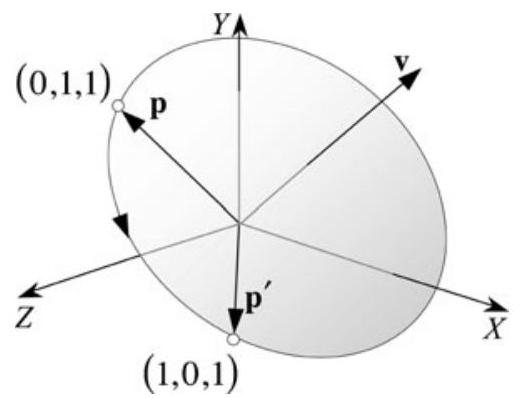
\includegraphics[max width=\textwidth]{2023_01_16_a848224efad29cd66460g-132}
\end{center}

$$
\begin{aligned}
& =\frac{1}{\sqrt{3}}\left[\frac{\sqrt{2}}{2}, \frac{\sqrt{2}}{2} \mathbf{j}\right]+\frac{1}{\sqrt{3}}\left[\frac{\sqrt{2}}{2}, \frac{\sqrt{2}}{2} \mathbf{i}\right] \\
& =\left[\frac{\sqrt{2}}{\sqrt{3}}, \frac{1}{\sqrt{6}} \mathbf{i}+\frac{1}{\sqrt{6}} \mathbf{j}\right]
\end{aligned}
$$

where

$$
s=\frac{\sqrt{2}}{\sqrt{3}}, \quad x=\frac{1}{\sqrt{6}}, \quad y=\frac{1}{\sqrt{6}}, \quad z=0
$$

which when substituted in $(7.15)$ gives

$$
\begin{aligned}
\mathbf{p}^{\prime} & =\left[\begin{array}{ccc}
2\left(s^{2}+x^{2}\right)-1 & 2(x y-s z) & 2(x z+s y) \\
2(x y+s z) & 2\left(s^{2}+y^{2}\right)-1 & 2(y z-s x) \\
2(x z-s y) & 2(y z+s x) & 2\left(s^{2}+z^{2}\right)-1
\end{array}\right]\left[\begin{array}{l}
x_{p} \\
y_{p} \\
z_{p}
\end{array}\right] \\
& =\left[\begin{array}{ccc}
\frac{2}{3} & \frac{1}{3} & \frac{2}{3} \\
\frac{1}{3} & \frac{2}{3} & -\frac{2}{3} \\
-\frac{2}{3} & \frac{2}{3} & \frac{1}{3}
\end{array}\right]\left[\begin{array}{l}
x_{p} \\
y_{p} \\
z_{p}
\end{array}\right] .
\end{aligned}
$$

Substituting the coordinates $(0,1,1)$ in $(7.24)$ gives

$$
\left[\begin{array}{l}
1 \\
0 \\
1
\end{array}\right]=\left[\begin{array}{ccc}
\frac{2}{3} & \frac{1}{3} & \frac{2}{3} \\
\frac{1}{3} & \frac{2}{3} & -\frac{2}{3} \\
-\frac{2}{3} & \frac{2}{3} & \frac{1}{3}
\end{array}\right]\left[\begin{array}{l}
0 \\
1 \\
1
\end{array}\right]
$$

which gives the point $(1,0,1)$.

One of the reasons for using a spherical interpolant is that it linearly interpolates the angle between the two unit-norm quaternions, which creates a constant-angular velocity between them. However, one of the problems with visualising quaternions is that they reside in a four-dimensional space and create a hyper-sphere with a radius equal to the quaternion's norm. With our 3D brains, this is difficult to visualise. Nevertheless, we can convince ourselves into thinking we see what is going on with a simple sketch, as shown in Fig. 7.14, where we see part of the hyper-sphere and two quaternions $q_{1}$ and $q_{2}$. In this example, the angle $\phi$ is a constant angle between two values of the interpolant $t$. The spherical interpolant also ensures that the norm Fig. 7.14 Spherical interpolation between $q_{1}$ and $q_{2}$
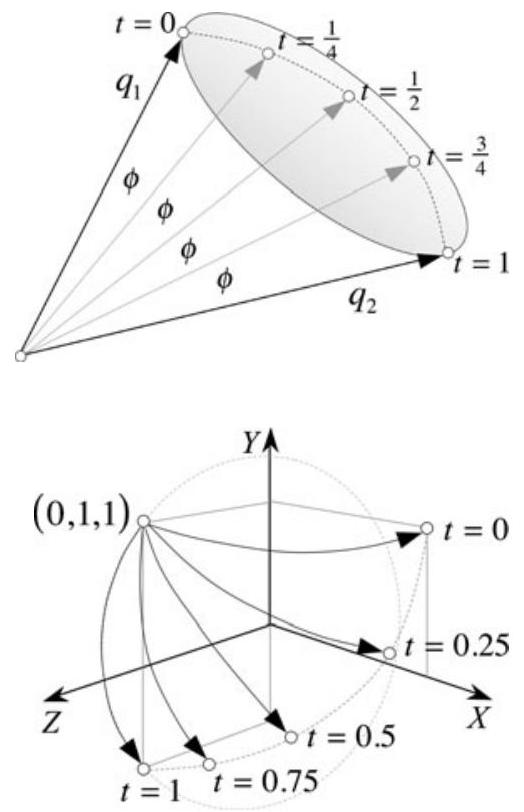
\includegraphics[max width=\textwidth, center]{2023_01_16_a848224efad29cd66460g-133}

Fig. 7.15 Sketch showing the actions of the interpolated quaternions of the interpolated quaternion remains constant at unity, preventing any unwanted scaling.

Figure $7.15$ provides another sketch to help visualise what is going on. For example, when $t=0$, the interpolated quaternion is $q_{1}$ which rotates the point $(0,1,1)$ to $(1,1,0)$, and when $t=1$, the interpolated quaternion is $q_{2}$ which rotates the point $(0,1,1)$ to $(0,-1,1)$. When $t=0.5$, the interpolated quaternion rotates the point $(0,1,1)$ to $(1,0,1)$ as computed above. Two other curves show what happens for $t=0.25$ and $t=0.75$.

A natural consequence of the interpolant is that the angle of rotation is $90^{\circ}$ for $t=0$ and $t=1$, but for $t=0.5$ the angle of rotation (eigenvalue) is approximately $70.5^{\circ}$. Corresponding angles arise for other values of $t$.

\section{将旋转矩阵转换为四元数}
The matrix transform equivalent to $q p q^{-1}$ is

$$
\begin{aligned}
q p q^{-1} & =\left[\begin{array}{ccc}
2\left(s^{2}+x^{2}\right)-1 & 2(x y-s z) & 2(x z+s y) \\
2(x y+s z) & 2\left(s^{2}+y^{2}\right)-1 & 2(y z-s x) \\
2(x z-s y) & 2(y z+s x) & 2\left(s^{2}+z^{2}\right)-1
\end{array}\right]\left[\begin{array}{l}
x_{p} \\
y_{p} \\
z_{p}
\end{array}\right] \\
& =\left[\begin{array}{lll}
a_{11} & a_{12} & a_{13} \\
a_{21} & a_{22} & a_{23} \\
a_{31} & a_{32} & a_{33}
\end{array}\right]\left[\begin{array}{l}
x_{p} \\
y_{p} \\
z_{p}
\end{array}\right] .
\end{aligned}
$$

Inspection of the matrix shows that by combining various elements we can isolate the terms of a quaternion $s, x, y, z$. For example, by adding the terms $a_{11}+a_{22}+a_{33}$ we obtain

$$
\begin{aligned}
a_{11}+a_{22}+a_{33} & =\left(2\left(s^{2}+x^{2}\right)-1\right)+\left(2\left(s^{2}+y^{2}\right)-1\right)+\left(2\left(s^{2}+z^{2}\right)-1\right) \\
& =6 s^{2}+2\left(x^{2}+y^{2}+z^{2}\right)-3 \\
& =4 s^{2}-1
\end{aligned}
$$

therefore,

$$
s=\pm \frac{1}{2} \sqrt{1+a_{11}+a_{22}+a_{33}} .
$$

To isolate $x, y$ and $z$ we employ

$$
\begin{aligned}
& x=\frac{1}{4 s}\left(a_{32}-a_{23}\right) \\
& y=\frac{1}{4 s}\left(a_{13}-a_{31}\right) \\
& z=\frac{1}{4 s}\left(a_{21}-a_{12}\right) .
\end{aligned}
$$

We can confirm their correctness using the matrix (7.25):

$$
\begin{aligned}
& \left[\begin{array}{lll}a_{11} & a_{12} & a_{13} \\a_{21} & a_{22} & a_{23} \\a_{31} & a_{32} & a_{33}\end{array}\right]=\left[\begin{array}{ccc}\frac{2}{3} & \frac{1}{3} & \frac{2}{3} \\\frac{1}{3} & \frac{2}{3} & -\frac{2}{3} \\-\frac{2}{3} & \frac{2}{3} & \frac{1}{3}\end{array}\right] \\
& s=\pm \frac{1}{2} \sqrt{1+a_{11}+a_{22}+a_{33}}=\pm \frac{1}{2} \sqrt{1+\frac{2}{3}+\frac{2}{3}+\frac{1}{3}}=\frac{\sqrt{2}}{\sqrt{3}} \\
& x=\frac{1}{4 s}\left(a_{32}-a_{23}\right)=\frac{\sqrt{3}}{4 \sqrt{2}}\left(\frac{2}{3}+\frac{2}{3}\right)=\frac{1}{\sqrt{6}} \\
& y=\frac{1}{4 s}\left(a_{13}-a_{31}\right)=\frac{\sqrt{3}}{4 \sqrt{2}}\left(\frac{2}{3}+\frac{2}{3}\right)=\frac{1}{\sqrt{6}} \\
& z=\frac{1}{4 s}\left(a_{21}-a_{12}\right)=\frac{\sqrt{3}}{4 \sqrt{2}}\left(\frac{1}{3}-\frac{1}{3}\right)=0
\end{aligned}
$$

which agree with the original values.

Say, for example, the value of $s$ had been close to zero, this could have made the values of $x, y, z$ unreliable. Consequently, other combinations are available:

$$
\begin{aligned}
& x=\pm \frac{1}{2} \sqrt{1+a_{11}-a_{22}-a_{33}} \\
& y=\frac{1}{4 x}\left(a_{12}+a_{21}\right) \\
& z=\frac{1}{4 x}\left(a_{13}+a_{31}\right)
\end{aligned}
$$

$$
\begin{aligned}
s & =\frac{1}{4 x}\left(a_{32}-a_{23}\right) \\
y & =\pm \frac{1}{2} \sqrt{1-a_{11}+a_{22}-a_{33}} \\
x & =\frac{1}{4 y}\left(a_{12}+a_{21}\right) \\
z & =\frac{1}{4 y}\left(a_{23}+a_{32}\right) \\
s & =\frac{1}{4 y}\left(a_{13}-a_{31}\right) \\
z & =\pm \frac{1}{2} \sqrt{1-a_{11}-a_{22}+a_{33}} \\
x & =\frac{1}{4 z}\left(a_{13}+a_{31}\right) \\
y & =\frac{1}{4 z}\left(a_{23}+a_{32}\right) \\
s & =\frac{1}{4 z}\left(a_{21}-a_{12}\right) .
\end{aligned}
$$

\section{欧拉角转换到四元数}
In Chap. 6 we discovered that the rotation transforms $\mathbf{R}_{\alpha, x}, \mathbf{R}_{\beta, y}$ and $\mathbf{R}_{\gamma, z}$ can be combined to create twelve triple combinations to represent a composite rotation. Now let's see how such a transform is represented by a quaternion.

To demonstrate the technique we must choose one of the twelve combinations, then the same technique can be used to convert other combinations. For example, let's choose the sequence $\mathbf{R}_{\gamma, z} \mathbf{R}_{\beta, y} \mathbf{R}_{\alpha, x}$ where the equivalent quaternions are

$$
\begin{aligned}
& q_{x}=\left[\cos \frac{1}{2} \alpha, \sin \frac{1}{2} \alpha \mathbf{i}\right] \\
& q_{y}=\left[\cos \frac{1}{2} \beta, \sin \frac{1}{2} \beta \mathbf{j}\right] \\
& q_{z}=\left[\cos \frac{1}{2} \gamma, \sin \frac{1}{2} \gamma \mathbf{k}\right]
\end{aligned}
$$

and

$$
q=q_{z} q_{y} q_{x}
$$

Expanding (7.26):

$$
\begin{aligned}
& q=\left[\cos \frac{1}{2} \gamma, \sin \frac{1}{2} \gamma \mathbf{k}\right]\left[\cos \frac{1}{2} \beta, \sin \frac{1}{2} \beta \mathbf{j}\right]\left[\cos \frac{1}{2} \alpha, \sin \frac{1}{2} \alpha \mathbf{i}\right] \\
& =\left[\cos \frac{1}{2} \gamma \cos \frac{1}{2} \beta,\right. \\
& \left.\cos \frac{1}{2} \gamma \sin \frac{1}{2} \beta \mathbf{j}+\cos \frac{1}{2} \beta \sin \frac{1}{2} \gamma \mathbf{k}-\sin \frac{1}{2} \gamma \sin \frac{1}{2} \beta \mathbf{i}\right]\left[\cos \frac{1}{2} \alpha, \sin \frac{1}{2} \alpha \mathbf{i}\right] \\
& =\left[\cos \frac{1}{2} \gamma \cos \frac{1}{2} \beta \cos \frac{1}{2} \alpha+\sin \frac{1}{2} \gamma \sin \frac{1}{2} \beta \sin \frac{1}{2} \alpha\right. \text {, } \\
& \cos \frac{1}{2} \gamma \cos \frac{1}{2} \beta \sin \frac{1}{2} \alpha \mathbf{i}+\cos \frac{1}{2} \alpha \cos \frac{1}{2} \gamma \sin \frac{1}{2} \beta \mathbf{j}+\cos \frac{1}{2} \alpha \cos \frac{1}{2} \beta \sin \frac{1}{2} \gamma \mathbf{k} \\
& \left.-\cos \frac{1}{2} \alpha \sin \frac{1}{2} \gamma \sin \frac{1}{2} \beta \mathbf{i}-\cos \frac{1}{2} \gamma \sin \frac{1}{2} \beta \sin \frac{1}{2} \alpha \mathbf{k}+\cos \frac{1}{2} \beta \sin \frac{1}{2} \gamma \sin \frac{1}{2} \alpha \mathbf{j}\right] \\
& =\left[\cos \frac{1}{2} \gamma \cos \frac{1}{2} \beta \cos \frac{1}{2} \alpha+\sin \frac{1}{2} \gamma \sin \frac{1}{2} \beta \sin \frac{1}{2} \alpha\right. \text {, } \\
& \left(\cos \frac{1}{2} \gamma \cos \frac{1}{2} \beta \sin \frac{1}{2} \alpha-\cos \frac{1}{2} \alpha \sin \frac{1}{2} \gamma \sin \frac{1}{2} \beta\right) \mathbf{i} \\
& \left(\cos \frac{1}{2} \alpha \cos \frac{1}{2} \gamma \sin \frac{1}{2} \beta+\cos \frac{1}{2} \beta \sin \frac{1}{2} \gamma \sin \frac{1}{2} \alpha\right) \mathbf{j} \\
& \left.\left(\cos \frac{1}{2} \alpha \cos \frac{1}{2} \beta \sin \frac{1}{2} \gamma-\cos \frac{1}{2} \gamma \sin \frac{1}{2} \beta \sin \frac{1}{2} \alpha\right) \mathbf{k}\right] \text {. }
\end{aligned}
$$

Now let's place the angles in a consistent sequence:

$$
\begin{aligned}
s & =\cos \frac{1}{2} \gamma \cos \frac{1}{2} \beta \cos \frac{1}{2} \alpha+\sin \frac{1}{2} \gamma \sin \frac{1}{2} \beta \sin \frac{1}{2} \alpha \\
x_{q} & =\cos \frac{1}{2} \gamma \cos \frac{1}{2} \beta \sin \frac{1}{2} \alpha-\sin \frac{1}{2} \gamma \sin \frac{1}{2} \beta \cos \frac{1}{2} \alpha \\
y_{q} & =\cos \frac{1}{2} \gamma \sin \frac{1}{2} \beta \cos \frac{1}{2} \alpha+\sin \frac{1}{2} \gamma \cos \frac{1}{2} \beta \sin \frac{1}{2} \alpha \\
z_{q} & =\sin \frac{1}{2} \gamma \cos \frac{1}{2} \beta \cos \frac{1}{2} \alpha-\cos \frac{1}{2} \gamma \sin \frac{1}{2} \beta \sin \frac{1}{2} \alpha
\end{aligned}
$$

where

$$
q=\left[s, x_{q} \mathbf{i}+y_{q} \mathbf{j}+z_{q} \mathbf{k}\right] .
$$

Let's test (7.27). We start with the three rotation transforms

$$
\begin{aligned}
\mathbf{R}_{\alpha, x} & =\left[\begin{array}{ccc}
1 & 0 & 0 \\
0 & \cos \alpha & -\sin \alpha \\
0 & \sin \alpha & \cos \alpha
\end{array}\right] \\
\mathbf{R}_{\beta, y} & =\left[\begin{array}{ccc}
\cos \beta & 0 & \sin \beta \\
0 & 1 & 0 \\
-\sin \beta & 0 & \cos \beta
\end{array}\right]
\end{aligned}
$$

$$
\mathbf{R}_{\gamma, z}=\left[\begin{array}{ccc}
\cos \gamma & -\sin \gamma & 0 \\
\sin \gamma & \cos \gamma & 0 \\
0 & 0 & 1
\end{array}\right]
$$

Then

$$
\begin{aligned}
& \mathbf{R}_{\gamma, z} \mathbf{R}_{\beta, y} \mathbf{R}_{\alpha, x} \\
&= {\left[\begin{array}{ccc}
\cos \gamma \cos \beta & -\sin \gamma \cos \alpha+\cos \gamma \sin \beta \sin \alpha & \sin \gamma \sin \alpha+\cos \gamma \sin \beta \cos \alpha \\
\sin \gamma \cos \beta & \cos \gamma \cos \alpha+\sin \gamma \sin \beta \sin \alpha & -\cos \gamma \sin \alpha+\sin \gamma \sin \beta \cos \alpha \\
-\sin \beta & \cos \beta \sin \alpha & \cos \beta \cos \alpha
\end{array}\right] . }
\end{aligned}
$$

Let's make $\alpha=\beta=\gamma=90^{\circ}$, then

$$
\mathbf{R}_{90^{\circ}, z} \mathbf{R}_{90^{\circ}, y} \mathbf{R}_{90^{\circ}, x}=\left[\begin{array}{ccc}
0 & 0 & 1 \\
0 & 1 & 0 \\
-1 & 0 & 0
\end{array}\right]
$$

which rotates points $90^{\circ}$ about the $y$-axis:

$$
\left[\begin{array}{l}
1 \\
1 \\
0
\end{array}\right]=\left[\begin{array}{ccc}
0 & 0 & 1 \\
0 & 1 & 0 \\
-1 & 0 & 0
\end{array}\right]\left[\begin{array}{l}
0 \\
1 \\
1
\end{array}\right]
$$

Now let's evaluate (7.27):

$$
\begin{aligned}
s & =\cos \frac{1}{2} \gamma \cos \frac{1}{2} \beta \cos \frac{1}{2} \alpha+\sin \frac{1}{2} \gamma \sin \frac{1}{2} \beta \sin \frac{1}{2} \alpha \\
& =\frac{\sqrt{2}}{2} \frac{\sqrt{2}}{2} \frac{\sqrt{2}}{2}+\frac{\sqrt{2}}{2} \frac{\sqrt{2}}{2} \frac{\sqrt{2}}{2} \\
& =\frac{\sqrt{2}}{2} \\
x_{q} & =\cos \frac{1}{2} \gamma \cos \frac{1}{2} \beta \sin \frac{1}{2} \alpha-\sin \frac{1}{2} \gamma \sin \frac{1}{2} \beta \cos \frac{1}{2} \alpha \\
& =0 \\
y_{q} & =\cos \frac{1}{2} \gamma \sin \frac{1}{2} \beta \cos \frac{1}{2} \alpha+\sin \frac{1}{2} \gamma \cos \frac{1}{2} \beta \sin \frac{1}{2} \alpha \\
& =\frac{\sqrt{2}}{2} \frac{\sqrt{2}}{2} \frac{\sqrt{2}}{2}+\frac{\sqrt{2}}{2} \frac{\sqrt{2}}{2} \frac{\sqrt{2}}{2} \\
& =\frac{\sqrt{2}}{2} \\
z_{q} & =\sin \frac{1}{2} \gamma \cos \frac{1}{2} \beta \cos \frac{1}{2} \alpha-\cos \frac{1}{2} \gamma \sin \frac{1}{2} \beta \sin \frac{1}{2} \alpha \\
& =0
\end{aligned}
$$

and

$$
q=\left[\frac{\sqrt{2}}{2}, \frac{\sqrt{2}}{2} \mathbf{j}\right]
$$

which is a quaternion that also rotates points $90^{\circ}$ about the $y$-axis.

\section{总结}
This chapter has been the focal point of the book where unit-norm quaternions have been used to rotate a vector about a quaternion's vector. It would have been useful if this could have been achieved by the simple product $q p$, like complex numbers. But as we saw, this only works when the quaternion is orthogonal to the vector. The product $q p q^{-1}$ —discovered by Hamilton and Cayley-works for all orientations between a quaternion and a vector. It is also relatively easy to compute. We also saw that the product can be represented as a matrix, which can be integrated with other matrices.

Perhaps one of the most interesting features of quaternions that has emerged in this chapter, is that their imaginary qualities are not required in any calculations, because they are embedded within the algebra.

The spherical interpolant provides a clever way to dynamically change a quaternion's axis and angle of rotation, but can be difficult to visualise as an animated sequence without access to a real-time display system.

The reverse product $q^{-1} p q$ reverses the angle of rotation, and is equivalent to changing the sign of the rotation angle in $q p q^{-1}$. Consequently, it can be used to rotate a frame of reference in the same direction as $q p q^{-1}$.

\subsection{操作符总结}
\subsubsection*{Rotating a point about a vector}
$$
\begin{aligned}
q & =[s, \mathbf{v}] \\
s^{2}+|\mathbf{v}|^{2} & =1 \\
p & =[0, \mathbf{p}] \\
q p q^{-1} & =\left[0,2(\mathbf{v} \cdot \mathbf{p}) \mathbf{v}+\left(2 s^{2}-1\right) \mathbf{p}+2 s \mathbf{v} \times \mathbf{p}\right] \\
q & =\left[\cos \frac{1}{2} \theta, \sin \frac{1}{2} \theta \hat{\mathbf{v}}\right] \\
p & =[0, \mathbf{p}] \\
q p q^{-1} & =[0,(1-\cos \theta)(\hat{\mathbf{v}} \cdot \mathbf{p}) \hat{\mathbf{v}}+\cos \theta \mathbf{p}+\sin \theta \hat{\mathbf{v}} \times \mathbf{p}]
\end{aligned}
$$

\subsubsection*{Rotating a frame about a vector}
$$
q^{-1} p q=[0,(1-\cos \theta)(\hat{\mathbf{v}} \cdot \mathbf{p}) \hat{\mathbf{v}}+\cos \theta \mathbf{p}-\sin \theta \hat{\mathbf{v}} \times \mathbf{p}]
$$

\subsubsection*{Matrix for rotating a point about a vector}
$$
\mathbf{p}^{\prime}=\left[\begin{array}{ccc}
1-2\left(y^{2}+z^{2}\right) & 2(x y-s z) & 2(x z+s y) \\
2(x y+s z) & 1-2\left(x^{2}+z^{2}\right) & 2(y z-s x) \\
2(x z-s y) & 2(y z+s x) & 1-2\left(x^{2}+y^{2}\right)
\end{array}\right]\left[\begin{array}{c}
x_{p} \\
y_{p} \\
z_{p}
\end{array}\right]
$$

\subsubsection*{Matrix for rotating a frame about a vector}
$$
\mathbf{p}^{\prime}=\left[\begin{array}{ccc}
1-2\left(y^{2}+z^{2}\right) & 2(x y+s z) & 2(x z-s y) \\
2(x y-s z) & 1-2\left(x^{2}+z^{2}\right) & 2(y z+s x) \\
2(x z+s y) & 2(y z-s x) & 1-2\left(x^{2}+y^{2}\right)
\end{array}\right]\left[\begin{array}{l}
x_{p} \\
y_{p} \\
z_{p}
\end{array}\right]
$$

\subsubsection*{Matrix for a quaternion product}
$$
\begin{aligned}
& q_{1} q_{2}=\mathbf{L}\left(q_{1}\right) q_{2}= {\left[\begin{array}{cccc}
s_{1} & -x_{1} & -y_{1} & -z_{1} \\
x_{1} & s_{1} & -z_{1} & y_{1} \\
y_{1} & z_{1} & s_{1} & -x_{1} \\
z_{1} & -y_{1} & x_{1} & s_{1}
\end{array}\right]\left[\begin{array}{l}
s_{2} \\
x_{2} \\
y_{2} \\
z_{2}
\end{array}\right] } \\
& q_{1} q_{2}=\mathbf{R}\left(q_{2}\right) q_{1}=\left[\begin{array}{cccc}
s_{2} & -x_{2} & -y_{2} & -z_{2} \\
x_{2} & s_{2} & z_{2} & -y_{2} \\
y_{2} & -z_{2} & s_{2} & x_{2} \\
z_{2} & y_{2} & -x_{2} & s_{2}
\end{array}\right]\left[\begin{array}{l}
s_{1} \\
x_{1} \\
y_{1} \\
z_{1}
\end{array}\right]
\end{aligned}
$$

\subsubsection*{Interpolating two quaternions}
$$
q=\frac{\sin (1-t) \theta}{\sin \theta} q_{1}+\frac{\sin t \theta}{\sin \theta} q_{2}
$$

where

$$
\begin{aligned}
\cos \theta & =\frac{q_{1} \cdot q_{2}}{\left|q_{1}\right|\left|q_{2}\right|} \\
& =\frac{s_{1} s_{2}+x_{1} x_{2}+y_{1} y_{2}+z_{1} z_{2}}{\left|q_{1}\right|\left|q_{2}\right|}
\end{aligned}
$$

\subsubsection*{Quaternion from a rotation matrix}
$$
\begin{aligned}
& s=\pm \frac{1}{2} \sqrt{1+a_{11}+a_{22}+a_{33}} \\
& x=\frac{1}{4 s}\left(a_{32}-a_{23}\right) \\
& y=\frac{1}{4 s}\left(a_{13}-a_{31}\right) \\
& z=\frac{1}{4 s}\left(a_{21}-a_{12}\right) \\
& x=\pm \frac{1}{2} \sqrt{1+a_{11}-a_{22}-a_{33}} \\
& y=\frac{1}{4 x}\left(a_{12}+a_{21}\right) \\
& z=\frac{1}{4 x}\left(a_{13}+a_{31}\right) \\
& s=\frac{1}{4 x}\left(a_{32}-a_{23}\right) \\
& y=\pm \frac{1}{2} \sqrt{1-a_{11}+a_{22}-a_{33}}
\end{aligned}
$$

$$
\begin{aligned}
x & =\frac{1}{4 y}\left(a_{12}+a_{21}\right) \\
z & =\frac{1}{4 y}\left(a_{23}+a_{32}\right) \\
s & =\frac{1}{4 y}\left(a_{13}-a_{31}\right) \\
z & =\pm \frac{1}{2} \sqrt{1-a_{11}-a_{22}+a_{33}} \\
x & =\frac{1}{4 z}\left(a_{13}+a_{31}\right) \\
y & =\frac{1}{4 z}\left(a_{23}+a_{32}\right) \\
s & =\frac{1}{4 z}\left(a_{21}-a_{12}\right)
\end{aligned}
$$

\subsubsection*{Eigenvector and eigenvalue}
$$
\begin{aligned}
x_{v} & =\left(a_{22}-1\right)\left(a_{33}-1\right)-a_{23} a_{32} \\
y_{v} & =\left(a_{33}-1\right)\left(a_{11}-1\right)-a_{31} a_{13} \\
z_{v} & =\left(a_{11}-1\right)\left(a_{22}-1\right)-a_{12} a_{21} \\
\cos \theta & =\frac{1}{2}\left(\operatorname{Tr}\left(q p q^{-1}\right)-1\right)
\end{aligned}
$$

\subsubsection*{Euler angles to quaternion}
Using the transform $\mathbf{R}_{\gamma, z} \mathbf{R}_{\beta, y} \mathbf{R}_{\alpha, x}$ :

$$
\begin{aligned}
s & =\cos \frac{1}{2} \gamma \cos \frac{1}{2} \beta \cos \frac{1}{2} \alpha+\sin \frac{1}{2} \gamma \sin \frac{1}{2} \beta \sin \frac{1}{2} \alpha \\
x_{q} & =\cos \frac{1}{2} \gamma \cos \frac{1}{2} \beta \sin \frac{1}{2} \alpha-\sin \frac{1}{2} \gamma \sin \frac{1}{2} \beta \cos \frac{1}{2} \alpha \\
y_{q} & =\cos \frac{1}{2} \gamma \sin \frac{1}{2} \beta \cos \frac{1}{2} \alpha+\sin \frac{1}{2} \gamma \cos \frac{1}{2} \beta \sin \frac{1}{2} \alpha \\
z_{q} & =\sin \frac{1}{2} \gamma \cos \frac{1}{2} \beta \cos \frac{1}{2} \alpha-\cos \frac{1}{2} \gamma \sin \frac{1}{2} \beta \sin \frac{1}{2} \alpha
\end{aligned}
$$

where

$$
q=\left[s, x_{q} \mathbf{i}+y_{q} \mathbf{j}+z_{q} \mathbf{k}\right]
$$

\section{样例}
Here are some further worked examples that employ the ideas described above.

Example 1 Use $q p$ to rotate $p=[0, \mathbf{j}] 90^{\circ}$ about the $x$-axis.

For this to work $q$ must be orthogonal to $p$ :

$$
\begin{aligned}
q & =[\cos \theta, \sin \theta \mathbf{i}] \\
& =[0, \mathbf{i}]
\end{aligned}
$$

and

$$
\begin{aligned}
p^{\prime} & =q p \\
& =[0, \mathbf{i}][0, \mathbf{j}] \\
& =[0, \mathbf{k}] .
\end{aligned}
$$

Example 2 Use $q p q^{-1}$ to rotate $p=[0, \mathbf{j}] 90^{\circ}$ about the $x$-axis.

For this to work:

$$
\begin{aligned}
q & =\left[\cos \frac{1}{2} \theta, \sin \frac{1}{2} \theta \mathbf{i}\right] \\
& =\left[\frac{\sqrt{2}}{2}, \frac{\sqrt{2}}{2} \mathbf{i}\right]
\end{aligned}
$$

and

$$
\begin{aligned}
p^{\prime} & =q p q^{-1} \\
& =\left[\frac{\sqrt{2}}{2}, \frac{\sqrt{2}}{2} \mathbf{i}\right][0, \mathbf{j}]\left[\frac{\sqrt{2}}{2},-\frac{\sqrt{2}}{2} \mathbf{i}\right] \\
& =\left[0, \frac{\sqrt{2}}{2} \mathbf{j}+\frac{\sqrt{2}}{2} \mathbf{k}\right]\left[\frac{\sqrt{2}}{2},-\frac{\sqrt{2}}{2} \mathbf{i}\right] \\
& =\left[0, \frac{\sqrt{2}}{2}\left(\frac{\sqrt{2}}{2} \mathbf{j}+\frac{\sqrt{2}}{2} \mathbf{k}\right)+\frac{1}{2} \mathbf{j}+\frac{1}{2} \mathbf{k}\right] \\
& =\left[0, \frac{1}{2} \mathbf{j}+\frac{1}{2} \mathbf{k}-\frac{1}{2} \mathbf{j}+\frac{1}{2} \mathbf{k}\right] \\
& =[0, \mathbf{k}]
\end{aligned}
$$

which agrees with the answer for Example 1.

Example 3 Evaluate the triple $q p q^{-1}$ for $p=[0, \mathbf{p}]$ and $q=\left[\cos \frac{1}{2} \theta, \sin \frac{1}{2} \theta \mathbf{v}\right]$, where $\theta=360^{\circ}$.

$$
\begin{aligned}
q & =[-1, \mathbf{0}] \\
q p q^{-1} & =[-1, \mathbf{0}][0, \mathbf{p}][-1, \mathbf{0}] \\
& =[0,-\mathbf{p}][-1, \mathbf{0}] \\
& =[0, \mathbf{p}]
\end{aligned}
$$

which confirms that the vector remains unmoved, as expected.

Example 4 Compute the matrix (7.15) for $q=\left[\frac{1}{2}, \frac{\sqrt{3}}{2} \mathbf{k}\right]$, and find its eigenvector and eigenvalue. From $q$

$$
\begin{aligned}
& s=\frac{1}{2}, \quad x=0, \quad y=0, \quad z=\frac{\sqrt{3}}{2} \\
& \mathbf{p}^{\prime}=\left[\begin{array}{ccc}2\left(s^{2}+x^{2}\right)-1 & 2(x y-s z) & 2(x z+s y) \\2(x y+s z) & 2\left(s^{2}+y^{2}\right)-1 & 2(y z-s x) \\2(x z-s y) & 2(y z+s x) & 2\left(s^{2}+z^{2}\right)-1\end{array}\right]\left[\begin{array}{l}x_{p} \\y_{p} \\z_{p}\end{array}\right] \\
& =\left[\begin{array}{ccc}-\frac{1}{2} & -\frac{\sqrt{3}}{2} & 0 \\\frac{\sqrt{3}}{2} & -\frac{1}{2} & 0 \\0 & 0 & 1\end{array}\right]\left[\begin{array}{l}x_{p} \\y_{p} \\z_{p}\end{array}\right] \text {. }
\end{aligned}
$$

If we plug in the point $(1,0,0)$ it is rotated about the $z$-axis by $120^{\circ}$ :

$$
\left[\begin{array}{c}
-\frac{1}{2} \\
\frac{\sqrt{3}}{2} \\
1
\end{array}\right]=\left[\begin{array}{ccc}
-\frac{1}{2} & -\frac{\sqrt{3}}{2} & 0 \\
\frac{\sqrt{3}}{2} & -\frac{1}{2} & 0 \\
0 & 0 & 1
\end{array}\right]\left[\begin{array}{l}
1 \\
0 \\
0
\end{array}\right]
$$

Using

$$
\begin{aligned}
\cos \theta & =\frac{1}{2}\left(\operatorname{Tr}\left(q p q^{-1}\right)-1\right) \\
& =\frac{1}{2}(0-1) \\
\theta & =120^{\circ}
\end{aligned}
$$

Using

$$
\begin{aligned}
x_{v} & =\left(a_{22}-1\right)\left(a_{33}-1\right)-a_{23} a_{32} \\
& =\left(-\frac{3}{2}\right)(0)-0 \\
& =0 \\
y_{v} & =\left(a_{33}-1\right)\left(a_{11}-1\right)-a_{31} a_{13} \\
& =(0)\left(-\frac{3}{2}\right)-0 \\
& =0 \\
z_{v} & =\left(a_{11}-1\right)\left(a_{22}-1\right)-a_{12} a_{21} \\
& =\left(-\frac{3}{2}\right)\left(-\frac{3}{2}\right)+\frac{\sqrt{3}}{2} \frac{\sqrt{3}}{2} \\
& =3
\end{aligned}
$$

which makes the eigenvector $3 \mathbf{k}$ and the eigenvalue $120^{\circ}$. Example 5 Find the half-way quaternion between $q_{1}=\left[\cos \frac{1}{2} \alpha, \sin \frac{1}{2} \alpha \mathbf{k}\right]$ and $q_{2}=$ $\left[\cos \frac{1}{2} \alpha, \sin \frac{1}{2} \alpha \mathbf{i}\right]$ when $\alpha=90^{\circ}$. Show that it is a unit-norm quaternion, and find its angle of rotation.

The angle between $q_{1}$ and $q_{2}$ is $\theta$ where

$$
\begin{aligned}
\cos \theta & =\frac{s_{1} s_{2}+x_{1} x_{2}+y_{1} y_{2}+z_{1} z_{2}}{\left|q_{1}\right|\left|q_{2}\right|} \\
& =\cos ^{2} \frac{1}{2} \alpha \\
& =0.5 \\
\theta & =60^{\circ} .
\end{aligned}
$$

Using

$$
\begin{aligned}
q & =\frac{\sin (1-t) \theta}{\sin \theta} q_{1}+\frac{\sin t \theta}{\sin \theta} q_{2} \\
& =\frac{\sin 30^{\circ}}{\sin 60^{\circ}}\left[\cos 45^{\circ}, \sin 45^{\circ} \mathbf{k}\right]+\frac{\sin 30^{\circ}}{\sin 60^{\circ}}\left[\cos 45^{\circ}, \sin 45^{\circ} \mathbf{i}\right] \\
& =\frac{1}{\sqrt{3}}\left[\frac{\sqrt{2}}{2}, \frac{\sqrt{2}}{2} \mathbf{k}\right]+\frac{1}{\sqrt{3}}\left[\frac{\sqrt{2}}{2}, \frac{\sqrt{2}}{2} \mathbf{i}\right] \\
& =\left[\frac{\sqrt{2}}{\sqrt{3}}, \frac{\sqrt{2}}{2 \sqrt{3}} \mathbf{i}+\frac{\sqrt{2}}{2 \sqrt{3}} \mathbf{k}\right] \\
& =\left[\frac{2}{\sqrt{6}}, \frac{1}{\sqrt{6}} \mathbf{i}+\frac{1}{\sqrt{6}} \mathbf{k}\right]
\end{aligned}
$$

The norm of $q$ is

$$
\begin{aligned}
|q| & =\left(\frac{2}{\sqrt{6}}\right)^{2}+\left(\frac{1}{\sqrt{6}}\right)^{2}+\left(\frac{1}{\sqrt{6}}\right)^{2} \\
& =\frac{2}{3}+\frac{1}{6}+\frac{1}{6} \\
& =1
\end{aligned}
$$

Therefore, $\cos \frac{1}{2} \alpha=\frac{\sqrt{2}}{\sqrt{3}}$ and $\sin \frac{1}{2} \alpha=\frac{1}{\sqrt{3}}$, and $\alpha \approx 70.5^{\circ}$.

Example 6 Convert the given matrix into a quaternion and identify its function.

$$
\mathbf{M}=\left[\begin{array}{ccc}
0 & 0 & 1 \\
0 & 1 & 0 \\
-1 & 0 & 0
\end{array}\right]
$$

therefore,

$$
\begin{aligned}
s & =\frac{1}{2} \sqrt{1+a_{11}+a_{22}+a_{33}} \\
& =\frac{1}{2} \sqrt{1+0+1+0}=\frac{\sqrt{2}}{2}
\end{aligned}
$$

$$
\begin{aligned}
x & =\frac{1}{4 s}\left(a_{32}-a_{23}\right) \\
& =\frac{\sqrt{2}}{4}(0+0)=0 \\
y & =\frac{1}{4 s}\left(a_{13}-a_{31}\right) \\
& =\frac{\sqrt{2}}{4}(1+1)=\frac{\sqrt{2}}{2} \\
z & =\frac{1}{4 s}\left(a_{21}-a_{12}\right) \\
& =\frac{\sqrt{2}}{4}(0+0)=0
\end{aligned}
$$

which is the quaternion $\left[\frac{\sqrt{2}}{2}, \frac{\sqrt{2}}{2} \mathbf{j}\right]$ which is a rotation of $90^{\circ}$ about the $y$-axis.


\chap{结论}
如果你已经阅读了前面的七章,读到了本章,那么你很可能已经理解了什么是四元数,以及如何用它绕任意轴旋转向量。我故意淡化了四元数的四维特性,因为这个特性与理解四元数是什么以及如何在入门级上操作它们无关。你现在应该能够对操作进行编码,并发现四元数在旋转阶段带来的好处。您还应该能够处理更高级的文本并发现其他应用程序。

很少有数学家能发明出令全世界大吃一惊的东西。因为正如我们在四元数的发明中所看到的那样, Gauss 曾尝试过四元数,但他太紧张了,不敢告诉任何人。同样, Grassmann 也一直在研究他自己的向量代数,并把他的想法写进了两本书,但他的写作风格太晦涩了,连数学家都看不懂! Rodrigues 被描述为一个“休闲的”数学家,也许只是为了好玩,他决定分析旋转的代数。在此过程中,他发现了一个与四元数乘积相同的半角解,比 Hamilton 早了三年。但最终,成功地将复数推广到更高维度的工作留给了 Hamilton 。他花了十多年的时间才找到最终的解决方案,尽管他是个天才,但他不知道三重积可能不是答案。幸运的是,他的坚韧和数学才华脱颖而出,赢得了胜利。

尽管 Hamilton 认为四元数将成为广泛科学应用的重要数学工具,但他们被 Gibbs描述的向量代数所忽视。 Hamilton 一定对四元数代数没有成为首选的向量系统感到失望,但他应该为能够为我们创造出今天的向量代数而感到无比自豪。

有趣的是,计算机时代,特别是计算机图形学的主题,为四元数提供了一个有用的应用。也许我们最终可以忘记欧拉旋转,使用一种直观、易于使用和有效的数学工具——四元数!




\begin{CJK}{UTF8}{gkai}
  \pdfbookmark{参考文献}{References}
  \chapter*{参考文献}
\end{CJK}
\begin{enumerate}
  \item Altmann, S.L.: Rotations, Quaternions and Double Groups. Dover, New York (2005). ISBN13: 978-0-486-44518-2 (1986)
  \item Altmann, S.L.: Rotations, Quaternions and Double Groups. Dover, New York (2005). ISBN13: 978-0-486-44518-2, p. $16(1986)$
  \item Altmann, S.L.: Rodrigues, and the quaternion scandal. Math. Mag. 62(5), 291-308 (1989)
  \item Altmann, S.L.: Icons and Symmetries. Clarendon Press, Oxford (1992)
  \item Altmann, S.L., Ortiz, E.L. (eds.): Mathematics and Social Utopias in France: Olinde Rodrigues and his Times. History of Mathematics, vol. 28. Am. Math. Soc., Providence (2005). ISBN-10: 0-8218-3860-1, ISBN-13: 978-0-8218-3860-0
  \item Argand, J.R.: \href{http://www-history.mcs.st-andrews.ac.uk/Mathematicians/Argand.html}{http://www-history.mcs.st-andrews.ac.uk/Mathematicians/Argand.html}
  \item Argand, J.R.: Essai sur une manière de représenter les quantités imaginaires dans les constructions géométriques, 2nd edn. Gauthier-Villars, Paris (1874)
  \item Cayley, A.: The Collected Mathematical Papers, vol. I, p. 586 (1848). Note 20
  \item Cheng, H., Gupta, K.C.: An historical note on finite rotations. Trans. ASME J. Appl. Mech. 56(1), 139-145 (1989)
  \item Crowe, M.J.: A History of Vector Analysis. Dover, New York (1994)

  \item Descartes, R.: La Géométrie (1637). There is an English translation by Michael Mahoney: Dover, New York (1979).

  \item Feynman, R.P.: Symmetry and physical laws. In: Feynman Lectures in Physics, vol. 1

  \item Gauss, C.F.: Mutation des Raumes. In: Carl Friedrich Gauss Werke, Achter Band, pp. $357-$ 361. König. Gesell. Wissen. Göttingen (1900). (1819)

  \item Hamilton, W.R.: In: Conway, A.W., Synge, J.L. (eds.) The Mathematical Papers of Sir William Rowan Hamilton, vol. I, Geometrical Optics; Conway, A.W., McDonnell, A.J. (eds.) vol. II, Dynamics; Halberstam, H., Ingram, R.E. (eds.) vol. III, Algebra, Cambridge University Press, Cambridge (1931, 1940, 1967) (1833)

  \item Hamilton, W.R.: \href{http://www-history.mcs.st-andrews.ac.uk/Mathematicians/Hamilton.html}{http://www-history.mcs.st-andrews.ac.uk/Mathematicians/Hamilton.html}

  \item Hamilton, W.R.: On Quaternions: Or a New System of Imaginaries in Algebra. Phil. Mag. 3rd ser. 25 (1844)

  \item Hamilton, W.R.: Lectures on Quaternions. Hodges \& Smith, Dublin (1853)

  \item Hamilton, W.R.: Elements of Quaternions. 2nd edn. Longmans, Green \& Co, London (18991901) (Jolly, C.J. (ed.) 2 vols.)

  \item Robinson, E.: Greek and English lexicon of the New Testament. \href{http://books.google.co.uk}{http://books.google.co.uk} (1825)

  \item Rodrigues, B.O.: Des lois géométriques qui régissent les déplacements d'un système solide dans l'espace, et de la variation des coordonnées provent de ses déplacements considérés indépendamment des causes qui peuvent les produire. J. Math. Pures Appl. 5, 380-440 (1840)

  \item Tait, P.G.: Elementary Treatise on Quaternions. Cambridge University Press, Cambridge (1867) 22. Wallis, J.: \href{http://www-history.mcs.st-andrews.ac.uk/Mathematicians/Wallis.html}{http://www-history.mcs.st-andrews.ac.uk/Mathematicians/Wallis.html}

  \item Wilson, E.B.: Vector Analysis. Yale University Press, New Haven (1901)

\end{enumerate}


%\include{num_pro}
%\include{mod_trans}



\clearpage
\end{CJK}
\end{document}